
\documentclass{article}



\usepackage{bm,verbatim}
\usepackage{algorithmic,algorithm}

\usepackage[final, nonatbib]{neurips_2024}





\usepackage{microtype}
\usepackage{wrapfig}
\usepackage{graphicx}
\usepackage{subcaption}
\usepackage{booktabs} %
\usepackage[colorlinks,citecolor=blue]{hyperref}
\newcommand{\theHalgorithm}{\arabic{algorithm}}
\usepackage{amsmath}
\usepackage{amssymb}
\usepackage{mathtools}
\usepackage{amsthm}
\usepackage{relsize}
\usepackage{physics}
\usepackage[normalem]{ulem}

\newcommand{\bx}{\mathbf{x}}
\newcommand{\bs}{\mathbf{s}}
\newcommand{\ba}{\mathbf{a}}
\newcommand{\bo}{\mathbf{o}}
\newcommand{\br}{\mathbf{r}}
\newcommand{\xtk}{\bx_t^{k_t}}
\newcommand{\bz}{\mathbf{z}}
\newcommand{\by}{\mathbf{y}}
\newcommand{\Exp}{\mathop{\mathlarger{\mathbb{E}}}}
\newcommand{\cN}{\mathcal{N}}
\newcommand{\cK}{\mathcal{K}}
\newcommand{\R}{\mathbb{R}}

\usepackage[capitalize,noabbrev]{cleveref}

\theoremstyle{plain}
\newtheorem{theorem}{Theorem}[section]
\newtheorem{proposition}[theorem]{Proposition}
\newtheorem{lemma}[theorem]{Lemma}
\newtheorem{claim}{Claim}
\newtheorem{corollary}[theorem]{Corollary}
\theoremstyle{definition}
\newtheorem{definition}[theorem]{Definition}
\newtheorem{assumption}[theorem]{Assumption}
\theoremstyle{remark}
\newtheorem{remark}{Remark}

\usepackage{color,verbatim}
\usepackage{color-edits}
\usepackage{titlesec}
\addauthor{ms}{magenta}
\addauthor{bc}{cyan}
\addauthor{dmm}{olive}
\addauthor{russt}{orange}
\addauthor{vs}{blue}
\newcommand{\yd}[1]{\textcolor{red}{#1}}

\usepackage[textsize=tiny]{todonotes}
\usepackage{ctable}%

\title{Diffusion Forcing: Next-token Prediction\\Meets Full-Sequence Diffusion}

\author{%
  Boyuan Chen \\
  MIT CSAIL\\
  \texttt{boyuanc@mit.edu} \\
  \And
  Diego Marti Monso\thanks{Work done as a visiting student at MIT.} \\
  Technical University of Munich\\
  \texttt{diego.marti@tum.de} \\
  \And
  Yilun Du \\
  MIT CSAIL\\
  \texttt{yilundu@mit.edu} \\
  \And
  Max Simchowitz \\
  MIT CSAIL\\
  \texttt{msimchow@mit.edu} \\
  \And
  Russ Tedrake \\
  MIT CSAIL\\
  \texttt{russt@mit.edu} \\
  \And
  Vincent Sitzmann \\
  MIT CSAIL\\
  \texttt{sitzmann@mit.edu} \\
}

\newcommand{\algo}{{Diffusion Forcing}}
\newcommand{\algoseq}{{Causal Diffusion Forcing}}
\newcommand{\algons}{Diffusion Forcing}
\newcommand{\algshort}{DF}
\newcommand{\algshortseq}{CDF}
\newcommand{\algopar}{(Causal) Diffusion Forcing}

\makeatletter
\renewcommand{\paragraph}{%
  \@startsection{paragraph}{4}%
  {\z@}{0ex \@plus 0ex \@minus 0.ex}{-0.5em}%
  {\normalfont\normalsize\bfseries}%
}
\makeatother


\begin{document}
\maketitle
\numberwithin{equation}{section}

\begin{abstract}
This paper presents \algons{}, a new training paradigm where a diffusion model is trained to denoise a set of tokens with \emph{independent} per-token noise levels.
We apply \algons{} to sequence generative modeling by training a causal next-token prediction model to generate one or several future tokens without fully diffusing past ones. Our approach is shown to combine the strengths of next-token prediction models, such as variable-length generation, with the strengths of full-sequence diffusion models, such as the ability to guide sampling to desirable trajectories. Our method offers a range of additional capabilities, such as (1) rolling-out sequences of continuous tokens, such as video, with lengths past the training horizon, where baselines diverge and (2) new sampling and guiding schemes that uniquely profit from \algons{}'s variable-horizon and causal architecture,  and which lead to marked performance gains in decision-making and planning tasks. In addition to its empirical success, our method is proven to optimize a variational lower bound on the likelihoods of all subsequences of tokens drawn from the true joint distribution. Project website: \url{https://boyuan.space/diffusion-forcing}

\end{abstract}

\documentclass[11pt]{report}
\usepackage[margin=2cm]{geometry}
\usepackage{graphicx}
\usepackage{float}
\usepackage{times}
\usepackage{url}
\usepackage[dvipsnames]{xcolor}
\usepackage{hyperref}

\newcommand{\specialcell}[2][c]{\begin{tabular}[#1]{@{}c@{}}#2\end{tabular}}

\newcommand{\Gap}{\texorpdfstring{\hfill}{}}
\newcommand{\Rec}{\texorpdfstring{{\small\emph{\color{ccai-blue}{\fbox{High Leverage}}}}}{}}
\newcommand{\HighRisk}{\texorpdfstring{{\small\emph{\color{ccai-yellow-darker}{\fbox{Uncertain Impact}}}}}{}}
\newcommand{\Longterm}{\texorpdfstring{{\small\emph{\color{ccai-green}{\fbox{Long-term}}}}}{}}

\begin{document}

\begin{abstract}
Climate change is one of the greatest challenges facing humanity, and we, as machine learning experts, may wonder how we can help. Here we describe how machine learning can be a powerful tool in reducing greenhouse gas emissions and helping society adapt to a changing climate. From smart grids to disaster management, we identify high impact problems where existing gaps can be filled by machine learning, in collaboration with other fields. Our recommendations encompass exciting research questions as well as promising business opportunities. We call on the machine learning community to join the global effort against climate change.
\vskip .5in
\end{abstract}

\part*{Introduction}
The effects of climate change are increasingly visible.\footnote{For a layman's introduction to the topic of climate change, see \cite{romm2018climate, archer2010climate}.} Storms, droughts, fires, and flooding have become stronger and more frequent \cite{field2012managing}. Global ecosystems are changing, including the natural resources and agriculture on which humanity depends. The 2018 intergovernmental report on climate change estimated that the world will face catastrophic consequences unless global greenhouse gas emissions are eliminated within thirty years \cite{ipcc_global_2018}. Yet year after year, these emissions rise.

Addressing climate change involves mitigation (reducing emissions) and adaptation (preparing for unavoidable consequences). Both are multifaceted issues. Mitigation of greenhouse gas (GHG) emissions requires changes to electricity systems, transportation, buildings, industry, and land use. Adaptation requires planning for resilience and disaster management, given an understanding of climate and extreme events. Such a diversity of problems can be seen as an opportunity: there are many ways to have an impact.

In recent years, machine learning (ML) has been recognized as a broadly powerful tool for technological progress. Despite the growth of movements applying ML and AI to problems of societal and global good,\footnote{See the AI for social good movement (e.g.~\cite{hager2019artificial, berendt2019ai}), ML for the developing world~\cite{de2018machine}, the computational sustainability movement (e.g.~\cite{kelling2018computational, joppa2017case, lassig2016computational, gomes2009computational, dietterich2009machine}, the American Meteorological Society's Committee on AI Applications to Environmental Science, and the field of Climate Informatics (\url{www.climateinformatics.org}) \cite{Monteleoni2013chapter}, as well as the relevant survey papers \cite{faghmous2014big, kaack2019challenges, ford2016opinion}.} there remains the need for a concerted effort to identify how these tools may best be applied to tackle climate change. Many ML practitioners wish to act, but are uncertain how. On the other side, many fields have begun actively seeking input from the ML community.

This paper aims to provide an overview of where machine learning can be applied with high impact in the fight against climate change, through either effective engineering or innovative research. The strategies we highlight include climate mitigation and adaptation, as well as meta-level tools that enable other strategies. In order to maximize the relevance of our recommendations, we have consulted experts across many fields (see \hyperref[sec:acknowledgments]{{\small{Acknowledgments}}}) in the preparation of this paper.


\begin{table}
\begin{small}
\begin{center}
\begin{tabular}{l l l l l l l l l l l l}  \toprule
     \multicolumn{2}{l}{ }
         & \small{\rotatebox{90}{\parbox{2.2cm}{Causal\\inference}}}
         & \small{\rotatebox{90}{\parbox{2.2cm}{Computer\\vision}}}
         & \small{\rotatebox{90}{\parbox{2.2cm}{Interpretable\\models}}}
         & \small{\rotatebox{90}{NLP}}
         & \small{\rotatebox{90}{\parbox{2.2cm}{RL \& Control}}}
        %  & \small{\rotatebox{90}{Robotics}}
         & \small{\rotatebox{90}{\parbox{2.2cm}{Time-series analysis}}}
         & \small{\rotatebox{90}{\parbox{2.2cm}{Transfer\\learning}}}
         & \small{\rotatebox{90}{\parbox{2.2cm}{Uncertainty\\quantification}}}
         & \small{\rotatebox{90}{\parbox{2.2cm}{Unsupervised\\learning}}}
    \\ \midrule
    \rowcolor{ccai-blue-lightest}
    \multicolumn{2}{l}{1 \hyperref[sec:electricity-systems]{Electricity systems}} 
        & % Causal inf
        &  % Comp vision
        & % Interpretable ml
        & % nlp
        & % rl + control
        & % time series
        & % transfer
        & % UQ
        & \\% unsupervised \ref{sub
    & \hyperref[sec:electricity-lowCarbon]{Enabling low-carbon electricity}
        & % Causal inf
        & $\bullet$% Comp vision
        & $\bullet$% % Interpretable ml
        & % % nlp
        & $\bullet$%% rl + control
        & $\bullet$% % time series
        & % transfer
        & $\bullet$% % UQ
        & $\bullet$\\% unsupervised 
    & \hyperref[sec:electricity-currentSystemImpact]{Reducing current-system impacts}
        & % Causal inf
        & $\bullet$% Comp vision
        & % Interpretable ml
        & % nlp
        & % rl + control
        & $\bullet$% % time series
        & % transfer
        & $\bullet$% % UQ
        & $\bullet$\\% unsupervised 
    & \hyperref[sec:electricity-developing]{Ensuring global impact}
        & % Causal inf
        & $\bullet$% Comp vision
        & % Interpretable ml
        & % nlp
        & % rl + control
        & % time series
        & $\bullet$ % transfer
        & % UQ
        & $\bullet$\\% unsupervised 
    \rowcolor{ccai-blue-lightest}
    \multicolumn{2}{l}{2 \hyperref[sec:transportation]{Transportation}} 
        & % Causal inf
        & % Comp vision
        &% Interpretable ml
        & % nlp
        & % rl + control
        & % time series
        & % transfer
        & % UQ
        & \\% unsupervised 
    & \hyperref[sec:TReducing]{Reducing transport activity}
        & % Causal inf
        & $\bullet$% Comp vision
        & % Interpretable ml
        & % nlp
        & % rl + control
        & $\bullet$% time series
        & % transfer
        & $\bullet$% UQ
        & $\bullet$\\% unsupervised     
   & \hyperref[sec:TEfficient]{Improving vehicle efficiency}
        & % Causal inf
        & $\bullet$% Comp vision
        & % Interpretable ml
        & % nlp
        & $\bullet$% rl + control
        & % time series
        & % transfer
        & % UQ
        & \\% unsupervised    
   & \hyperref[sec:TFuels]{Alternative fuels \& electrification}
        & % Causal inf
        & % Comp vision
        & % Interpretable ml
        & % nlp
        & $\bullet$% rl + control
        & % time series
        & % transfer
        & % UQ
        & $\bullet$ \\% unsupervised    
   & \hyperref[sec:modalshift]{Modal shift}
        & $\bullet$% Causal inf
        & $\bullet$% Comp vision
        & % Interpretable ml
        & % nlp
        & % rl + control
        & $\bullet$% time series
        & % transfer
        & $\bullet$% UQ
        & \\% unsupervised    
    \rowcolor{ccai-blue-lightest}
    \multicolumn{2}{l}{3 \hyperref[sec:buildings-cities]{Buildings and cities}} 
        & % Causal inf
        & % Comp vision
        & % Interpretable ml
        & % nlp
        & % rl + control
        & % time series
        & % transfer
        & % UQ
        & \\% unsupervised 
    & \hyperref[sec:indv]{Optimizing buildings}
        & $\bullet$% Causal inf
        & % Comp vision
        & % Interpretable ml
        & % nlp
        & $\bullet$% rl + control
        & $\bullet$% time series
        & $\bullet$% transfer
        & % UQ
        & \\% unsupervised 
    & \hyperref[sec:distr]{Urban planning}
        & % Causal inf
        & $\bullet$% Comp vision
        & % Interpretable ml
        & % nlp
        & % rl + control
        & $\bullet$% time series
        & $\bullet$% transfer
        & % UQ
        & $\bullet$\\% unsupervised 
    & \hyperref[sec:cities]{The future of cities}
        & % Causal inf
        & % Comp vision
        & % Interpretable ml
        & $\bullet$%% nlp
        & % rl + control
        & %% time series
        & $\bullet$%% transfer
        & $\bullet$% UQ
        & $\bullet$\\% unsupervised 
    \rowcolor{ccai-blue-lightest}
    \multicolumn{2}{l}{4 \hyperref[sec:industry]{Industry}} 
        & % Causal inf
        & % Comp vision
        & % Interpretable ml
        & % nlp
        & % rl + control
        & % time series
        & % transfer
        & % UQ
        & \\% unsupervised 
    & \hyperref[sec:supplychains]{Optimizing supply chains}
        & % Causal inf
        & $\bullet$ %% Comp vision
        & % Interpretable ml
        & % nlp
        & $\bullet$ % rl + control
        & $\bullet$ % time series
        & % transfer
        & % UQ
        & \\% unsupervised 
    & \hyperref[sec:materialsandconstruction]{Improving materials}
        & %% Causal inf
        & % Comp vision
        & % Interpretable ml
        & % nlp
        & % rl + control
        & % time series
        & %% transfer
        & % UQ
        & $\bullet$ \\% unsupervised 
    & \hyperref[sec:demandresponse]{Production \& energy}
        & %% Causal inf
        & $\bullet$%% Comp vision
        & $\bullet$ %% Interpretable ml
        & % nlp
        & $\bullet$% rl + control
        & %% time series
        & %% transfer
        & % UQ
        & \\% unsupervised 
    \rowcolor{ccai-blue-lightest}
    \multicolumn{2}{l}{5 \hyperref[sec:afolu]{Farms \& forests}} 
        & % Causal inf
        & % Comp vision
        & % Interpretable ml
        & % nlp
        & % rl + control
        & % time series
        & % transfer
        & % UQ
        & \\% unsupervised 
    & \hyperref[sec:emissions-detection]{Remote sensing of emissions}
        & % Causal inf
        & $\bullet$% Comp vision
        & % Interpretable ml
        & % nlp
        & % rl + control
        & % time series
        & % transfer
        & % UQ
        & \\% unsupervised 
    & \hyperref[sec:agriculture]{Precision agriculture}
        & % Causal inf
        & $\bullet$% Comp vision
        & % Interpretable ml
        & % nlp
        & $\bullet$% rl + control
        & $\bullet$% time series
        & % transfer
        & % UQ
        & \\% unsupervised 
    & \hyperref[sec:peatlands]{Monitoring peatlands}
        & % Causal inf
        & $\bullet$% Comp vision
        & % Interpretable ml
        & % nlp
        & % rl + control
        & % time series
        & % transfer
        & % UQ
        & \\% unsupervised 
    & \hyperref[sec:forests]{Managing forests}
        & % Causal inf
        & $\bullet$% Comp vision
        & % Interpretable ml
        & % nlp
        & $\bullet$ % rl + control
        & $\bullet$ % time series
        & % transfer
        & % UQ
        & \\% unsupervised 
    \rowcolor{ccai-blue-lightest}
    \multicolumn{2}{l}{6 \hyperref[sec:ccs]{Carbon dioxide removal}}
        & % Causal inf
        & % Comp vision
        & % Interpretable ml
        & % nlp
        & % rl + control
        & % time series
        & % transfer
        & % UQ
        & \\
    & \hyperref[sec:ccs]{Direct air capture}
        & % Causal inf
        & % Comp vision
        & % Interpretable ml
        & % nlp
        & % rl + control
        & % time series
        & % transfer
        & % UQ
        & $\bullet$\\% unsupervised 
    & \hyperref[subsubsec: sequestrativervin]{Sequestering~\cd}
        & % Causal inf
        & $\bullet$% Comp vision
        & % Interpretable ml
        & % nlp
        & % rl + control
        & % time series
        & % transfer
        & $\bullet$% UQ
        & $\bullet$\\% unsupervised 
    \rowcolor{ccai-blue-lightest}
    \multicolumn{2}{l}{7 \hyperref[sec: climate prediction]{Climate prediction}} 
        & % Causal inf
        & % Comp vision
        & % Interpretable ml
        & % nlp
        & % rl + control
        & % time series
        & % transfer
        & % UQ
        & \\% unsupervised 
    & \hyperref[sec:climate-models-params]{Uniting data, ML \& climate science}
        & % Causal inf
        & $\bullet$% Comp vision
        & $\bullet$% Interpretable ml
        & % nlp
        & % rl + control
        & $\bullet$% time series
        & % transfer
        & $\bullet$% UQ
        & \\% unsupervised 
    & \hyperref[sec:models-extreme-events]{Forecasting extreme events}
        & % Causal inf
        & $\bullet$% Comp vision
        & $\bullet$% Interpretable ml
        & % nlp
        & % rl + control
        & $\bullet$% time series
        & % transfer
        & $\bullet$% UQ
        & \\% unsupervised 
    \rowcolor{ccai-blue-lightest}
    \multicolumn{2}{l}{8 \hyperref[sec:societal-impacts]{Societal impacts}} 
        & % Causal inf
        & % Comp vision
        & % Interpretable ml
        & % nlp
        & % rl + control
        & % time series
        & % transfer
        & % UQ
        & \\% unsupervised 
    & \hyperref[subsub:ecology]{Ecology}
        & % Causal inf
        & $\bullet$% Comp vision
        & % Interpretable ml
        & % nlp
        & % rl + control
        & % time series
        & $\bullet$% transfer
        & % UQ
        & \\% unsupervised 
    & \hyperref[subsub:infrastructure]{Infrastructure}
        & % Causal inf
        & % Comp vision
        & % Interpretable ml
        & % nlp
        & $\bullet$% rl + control
        & $\bullet$% time series
        & % transfer
        & $\bullet$% UQ
        & \\% unsupervised 
    & \hyperref[subsub:social_systems]{Social systems}
        & % Causal inf
        & $\bullet$% Comp vision
        & % Interpretable ml
        & % nlp
        & % rl + control
        & $\bullet$% time series
        & % transfer
        & % UQ
        & $\bullet$\\% unsupervised 
    & \hyperref[subsub:crisis]{Crisis}
        & % Causal inf
        & $\bullet$% Comp vision
        & % Interpretable ml
        & $\bullet$% nlp
        & % rl + control
        & % time series
        & % transfer
        & % UQ
        & \\% unsupervised 
    \rowcolor{ccai-blue-lightest}
    \multicolumn{2}{l}{9 \hyperref[sec:geoengineering]{Solar geoengineering}} 
        & % Causal inf
        & % Comp vision
        & % Interpretable ml
        & % nlp
        & % rl + control
        & % time series
        & % transfer
        & % UQ
        & \\% unsupervised 
    & \hyperref[subsub:better-aerosols]{Understanding \& improving aerosols}
        & % Causal inf
        & % Comp vision
        & % Interpretable ml
        & % nlp
        & % rl + control
        & $\bullet$% time series
        & % transfer
        & $\bullet$% UQ
        & \\% unsupervised 
    & \hyperref[subsub:planetary-control]{Engineering a planetary control system}
        & % Causal inf
        & % Comp vision
        & % Interpretable ml
        & % nlp
        & $\bullet$% rl + control
        & % time series
        & % transfer
        & $\bullet$% UQ
        & \\% unsupervised 
    & \hyperref[subsub:impact-models]{Modeling impacts}
        & % Causal inf
        & % Comp vision
        & % Interpretable ml
        & % nlp
        & % rl + control
        & $\bullet$% time series
        & % transfer
        & $\bullet$% UQ
        & \\% unsupervised 
    \rowcolor{ccai-blue-lightest}
    \multicolumn{2}{l}{10 \hyperref[sec:tools-individuals]{Individual action}} 
        & % Causal inf
        & % Comp vision
        & % Interpretable ml
        & % nlp
        & % rl + control
        & % time series
        & % transfer
        & % UQ
        & \\% unsupervised 
    & \hyperref[sec:personal_carbon_footprint]{Understanding personal footprint}
        & $\bullet$% Causal inf
        & % Comp vision
        & % Interpretable ml
        & $\bullet$% nlp
        & $\bullet$% rl + control
        & $\bullet$% time series
        & % transfer
        & % UQ
        & \\% unsupervised 
    & \hyperref[sec:behavior_change]{Facilitating behavior change}
        & % Causal inf
        & % Comp vision
        & % Interpretable ml
        & $\bullet$% nlp
        & % rl + control
        & % time series
        & % transfer
        & % UQ
        & $\bullet$\\% unsupervised 
    \rowcolor{ccai-blue-lightest}
    \multicolumn{2}{l}{11 \hyperref[sec:toolsforsociety]{Collective decisions}} 
        & % Causal inf
        & % Comp vision
        & % Interpretable ml
        & % nlp
        & % rl + control
        & % time series
        & % transfer
        & % UQ
        &  \\% unsupervised 
    & \hyperref[sec:coordination]{Modeling social interactions}
        & % Causal inf
        & % Comp vision
        & $\bullet$ % Interpretable ml
        & % nlp
        & $\bullet$ % rl + control
        & % time series
        & % transfer
        & % UQ
        & \\% unsupervised 
    & \hyperref[sec:decisionmaking]{Informing policy}
        & $\bullet$ % Causal inf
        & $\bullet$ % Comp vision
        & % Interpretable ml
        & $\bullet$% nlp
        & % rl + control
        & % time series
        & % transfer
        & $\bullet$% UQ
        & $\bullet$\\% unsupervised 
    & \hyperref[subsec:markets]{Designing markets}
        & % Causal inf
        & % Comp vision
        & % Interpretable ml
        & % nlp
        & $\bullet$% rl + control
        & $\bullet$% time series
        & % transfer
        & % UQ
        & $\bullet$\\% unsupervised 
    \rowcolor{ccai-blue-lightest}
    \multicolumn{2}{l}{12 \hyperref[sec:education]{Education}} 
        & % Causal inf
        & % Comp vision
        & % Interpretable ml
        & $\bullet$% nlp
        & $\bullet$% rl + control
        & % time series
        & % transfer
        & % UQ
        & \\% unsupervised 
    \rowcolor{ccai-blue-lightest}
    \multicolumn{2}{l}{13 \hyperref[sec:finance]{Finance}} 
        & % Causal inf
        & % Comp vision
        & % Interpretable ml
        & $\bullet$% nlp
        & % rl + control
        & $\bullet$% time series
        & % transfer
        & $\bullet$% UQ
        & \\% unsupervised 
    \bottomrule
\end{tabular}
\caption{Climate change solution domains, corresponding to sections of this paper, matched with selected areas of ML that are relevant to each. }
\label{tab:summary}
\end{center}
\end{small}
\end{table}


\subsection*{Who is this paper written for?}

We believe that our recommendations will prove valuable to several different audiences (detailed below). In our writing, we have assumed some familiarity with basic terminology in machine learning, but do not assume any prior familiarity with application domains (such as agriculture or electric grids).\\

\textbf{Researchers and engineers:}
We identify many problems that require conceptual innovation and can advance the field of ML, as well as being highly impactful. For example, we highlight how climate models afford an exciting domain for interpretable ML (see \S\ref{sec: climate prediction}).
We encourage researchers and engineers across fields to use their expertise in solving urgent problems relevant to society.\\

\textbf{Entrepreneurs and investors:} We identify many problems where existing ML techniques could have a major impact without further research, and where the missing piece is deployment. We realize that some of the recommendations we offer here will make valuable startups and nonprofits. For example, we highlight techniques for providing fine-grained solar forecasts for power companies (see \S\ref{sec:electricity-lowCarbon}), tools for helping reduce personal energy consumption (see \S\ref{sec:behavior_change}), and predictions for the financial impacts of climate change (see \S\ref{sec:finance}). We encourage entrepreneurs and investors to fill what is currently a wide-open space.\\

\textbf{Corporate leaders:} We identify problems where ML can lead to massive efficiency gains if adopted at scale by corporate players. For example, we highlight means of optimizing supply chains to reduce waste (see \S\ref{sec:supplychains}) and software/hardware tools for precision agriculture (see \S\ref{sec:agriculture}). We encourage corporate leaders to take advantage of opportunities offered by ML to benefit both the world and the bottom line.\\

\textbf{Local and national governments:} We identify problems where ML can improve public services, help gather data for decision-making, and guide plans for future development. For example, we highlight intelligent transportation systems (see \S\ref{sec:modalshift}), techniques for automatically assessing the energy consumption of buildings in cities (see \S\ref{sec:indv}),
and tools for improving disaster management (see \S\ref{subsub:crisis}). We encourage governments to consult ML experts while planning infrastructure and development, as this can lead to better, more cost-effective outcomes. We further encourage public entities to release data that may be relevant to climate change mitigation and adaptation goals.\\

\subsection*{How to read this paper} \label{sub:howtoread}
The paper is broken into sections according to application domain (see Table \ref{tab:summary}). To help the reader, we have also included the following flags at the level of individual strategies.
\begin{itemize}
\item \textbf{\Rec} $\,$ denotes bottlenecks that domain experts have identified in climate change mitigation or adaptation and that we believe to be particularly well-suited to tools from ML. These areas may be especially fruitful for ML practitioners wishing to have an outsized impact, though applications not marked with this flag are also valuable and should be pursued.
\item \textbf{\Longterm} $\,$ denotes applications that will have their primary impact after 2040. While extremely important, these may in some cases be less pressing than those which can help act on climate change in the near term.
\item \textbf{\HighRisk} $\,$ denotes applications where the impact on GHG emissions is uncertain (for example, the \emph{Jevons paradox} may apply\footnote{The Jevons paradox in economics refers to a situation where increased efficiency nonetheless results in higher overall demand. For example, autonomous vehicles could cause people to drive far more, so that overall GHG emissions could increase even if each ride is more efficient. In such cases, it becomes especially important to make use of specific policies, such as carbon pricing, to direct new technologies and the ML behind them. See also the literature on rebound effects and induced demand.}) or where there is  potential for undesirable side effects (\emph{negative externalities}).
\end{itemize}

These flags should not be taken as definitive; they represent our understanding of more rigorous analyses within the domains we consider, combined with our subjective evaluation of the potential role of ML in these various applications.

Despite the length of the paper, we cannot cover everything. There will certainly be many applications that we have not considered, or that we have erroneously dismissed. We look forward to seeing where future work leads.

\subsection*{A call for collaboration}

All of the problems we highlight in this paper require collaboration across fields. As the language used to refer to problems often varies between disciplines, we have provided keywords and background reading within each section of the paper. Finding collaborators and relevant data can sometimes be difficult; for additional resources, please visit the website that accompanies this paper: \url{https://www.climatechange.ai/}.

Collaboration makes it easier to develop effective strategies. Working with domain experts reduces the chance of using powerful tools when simple tools will do the job, of working on a problem that isn't actually relevant to practitioners, of overly simplifying a complex issue,
or of failing to anticipate risks.

Collaboration can also help ensure that new work reaches the audience that will use it. To be impactful, ML code should be accessible and published using a language and a platform that are already popular with the intended users. For maximal impact, new code can be integrated into an existing, widely used tool.

We emphasize that machine learning is not a silver bullet. The applications we highlight are impactful, but no one solution will ``fix'' climate change. There are also many areas of action where ML is inapplicable, and we omit these entirely. Furthermore, technology alone is not enough -- technologies that would address climate change have been available for years, but have largely not been adopted at scale by society. While we hope that ML will be useful in reducing the costs associated with climate action, humanity also must decide to act.

\end{document}

\section{Related Work}
\label{section:related_work}
The development of Llama 3 builds on a large body of prior work studying foundation models for language, images, videos, and speech.
A comprehensive overview of that work is outside the scope of this paper; we refer the reader to \citet{bordes2024vlm,madan2024foundation,LLMSurvey} for such overviews.
Below, we briefly outline seminal works that directly influenced the development of Llama 3.

\subsection{Language}
\label{section:related_work_language}

\textbf{Scale.}
Llama 3 follows the enduring trend of applying straightforward methods at ever increasing scales in foundation models. Improvements are driven by increased compute and improved data, with the 405B model using almost fifty times the pre-training compute budget of Llama 2 70B. Despite containing 405B parameters, our largest Llama 3 in fact contains fewer parameters than earlier and much less performant models such as PALM~\citep{chowdhery2023palm}, due to better understanding of scaling laws~\citep{kaplan2020scaling,hoffmann2022chinchilla}. Little is publicly known about the size of other frontier models, such as Claude 3 or GPT 4~\citep{openai2023gpt4}, but overall performance is compareable. 

\textbf{Small models.}
Developments in smaller models have paralleled those in large models. 
Models with fewer parameters can dramatically improve inference cost and simplify deployment~\citep{mehta2024openelm,team2024gemma}.
The smaller Llama 3 models achieve this by training far beyond the point of compute optimal training, effectively trading training compute for inference efficiency.
An alternative path is to distill larger models into smaller ones, as in Phi~\citep{abdin2024phi}.

\textbf{Architectures.}
While Llama 3 makes minimal architectural modifiations to compared to Llama 2, other recent foundation models have explored other designs. Most notably, mixture of experts architectures~\citep{shazeer2017moe,lewis2021base,fedus2022switch,zhou2022mixture} can be used as an efficient way to increase the capacity of a models, such as in Mixtral~\citep{jiang2024mixtral} and Arctic~\citep{snowflakearctic}. Llama 3 outperforms these models, suggesting that dense architectures are not the limiting factor, but there remain numerous trade offs in terms of training and inference efficiency, and model stability at scale.

\textbf{Open source.}
Open weights foundation models have rapidly improved over the last year, with Llama3-405B now competitive with the current closed weight state-of-the-art. 
Numerous model families have recently been developed, including Mistral~\citep{jiang2023mistral}, Falcon~\citep{almazrouei2023falcon}, MPT~\citep{databricksmpt}, Pythia~\citep{biderman2023pythia}, Arctic~\citep{snowflakearctic}, OpenELM~\citep{mehta2024openelm}, OLMo~\citep{groeneveld2024olmoacceleratingsciencelanguage}, StableLM~\citep{bellagente2024stable}, OpenLLaMA~\citep{openlm2023openllama}, Qwen~\citep{bai2023qwen}, Gemma~\citep{team2024gemma}, Grok~\citep{xaigrok}, and Phi~\citep{abdin2024phi}.

\textbf{Post-training.}
Post-training \llamathree follows the established strategy of instruction tuning~\citep{chung2022scalinginstruction,ouyang2022instructgpt} followed by alignment with human feedback~\citep{kaufmann2023survey}. While some studies have shown the surprising effectiveness of lightweight alignment procedures~\citep{zhou2024lima}, \llamathree uses millions of human instructions and preference judgments to improve the pre-trained model, including techniques such as rejection sampling~\citep{constitutional-ai-bai}, supervised finetuning~\citep{sanh2022multitask}, and Direct Preference Optimization~\citep{rafailov2023dpo}. In order to curate these instruction and preference examples, we deploy earlier versions of \llamathree to filter~\citep{liu2024makesgooddataalignment}, re-write~\citep{pan2024selfcorrection}, or generate prompts and responses~\citep{liu2024bestpractices} and apply these techniques through multiple rounds of post-training.


\subsection{Multimodality}
\label{section:related_work_multimodality}
Our experiments with multimodal capabilities for Llama 3 are part of a long line of work on foundation models that jointly model multiple modalities.

\textbf{Images.} 
A substantial body of work has trained image-recognition models on large amounts of image-text pairs, for example, \citet{Mahajan_2018_ECCV,xiao2024florence,chameleon2024,openai2023gpt4blog}.
\citet{radford2021learning} presented one of the first models to jointly embed images and text via contrastive learning. 
More recently, a series of models has studied approaches similar to the one used in Llama 3, for example, \citet{alayrac2022flamingo,dai2023instructblip,liu2023llava,liu2023improvedllava,yang2023mmreact,ye2023mplug,zhu2023minigpt}.
Our approach in Llama 3 combines ideas from many of these papers to achieve results that are comparable with Gemini 1.0 Ultra \citep{gemini2023gemini} and GPT-4 Vision \citep{openai2023gpt4blog}; see Section~\ref{section:results_image_recognition}.


\textbf{Video.}
Although video inputs are supported by an increasing number of foundation models \citep{gemini2023gemini,openai2023gpt4blog}, the body of work on joint modeling of videos and language is not that large.
Akin to Llama 3, most current studies adopt an adapter approach to align video and language representations and unlock question-answering and reasoning about videos \citep{lin2023video,li2023videochat,Maaz2023VideoChatGPT,zhang2023videollama,zhao2022lavila}.
We find that such approaches produce results that are competitive with the state-of-the-art; see Section~\ref{section:results_video_recognition}.

\textbf{Speech.}
Our work also fits in a larger body of work combining language and speech modeling.
Earlier joint models of text and speech include AudioPaLM \citep{rubenstein2023audiopalm}, VioLA \citep{wang2023viola}, VoxtLM \cite{maiti2023voxtlm}, SUTLM \citep{chou2023sutlm}, and Spirit-LM \citep{nguyen2024spirit}.
Our work builds on prior compositional approaches to combining speech and language like \citet{fathullah2024audiochatllama}.
Unlike most prior work, we opt to not finetune the language model itself for speech tasks as doing so may lead to contention on non-speech tasks.
We find that at larger model scales, strong performances are attainable even without such finetuning; see Section~\ref{section:results_speech}.


\section{Method}

\subsection{Noising as partial masking}
Recall that \emph{masking} is the practice of occluding a subset of data, such as patches of an image~\cite{he2022masked} or timesteps in a sequence~\cite{bert, t5}, and training a model to recover unmasked portions. 
Without loss of generality, we can view any collection of tokens, sequential or not, as an ordered set indexed by $t$.
Training next-token prediction with teacher forcing can then be interpreted as masking each token $\bx_t$ at time $t$ and making predictions from the past  $\bx_{1:t-1}$. Restricted to sequences, we refer to all these practices as \emph{masking along the time axis}. We can also view full-sequence forward diffusion, i.e., gradually adding noise to the data $ \bx^0_{1:T} \equiv \bx_{1:T}$, as a form of \emph{partial masking}, which we refer to as \emph{masking along the noise axis}. Indeed, after $K$ steps of noising, $\bx^K_{1:T}$ is (approximately) pure white noise without information about the original data.

We establish a unified view along both axes of masking (see Fig.~\ref{fig:method}).  We denote  $\bx_{1:T}$ for a sequence of tokens, where the subscript indicates the time axis. As above, $\xtk$ denotes $\bx_t$ at noise level $k_t$ under the forward diffusion process~\eqref{eqn:forward_diffusion};  $\bx_t^0 = \bx$ is the unnoised token, and  $\bx^K_t$ is white noise $ \mathcal{N}(0, \mathbf{I})$. Thus, $(\xtk)_{1 \le t \le T}$ denotes a sequence of noisy observations where each token has a \emph{different} noise level $k_t$, which can be seen as the degree of \emph{partial masking} applied to each token through noising.

\subsection{\algons{}: different noise levels for different tokens}
\emph{\algo{}} ({\algshort}) is a framework for training and sampling arbitrary sequence lengths of noisy tokens $(\xtk)_{1 \le t \le T}$, where critically, \emph{the noise level $k_t$ of each token can vary by time step}. 
In this paper, we focus on time series data, and thus instantiate \algo{} with causal architectures (where $\xtk$ depends only on past noisy tokens), which we call \emph{\algoseq{}} ({\algshortseq{}}).
For simplicity, we focus on a minimal implementation with a vanilla Recurrent Neural Network (RNN) ~\cite{gru}. Potential transformer implementation of \algo{} is also possible but we defer its discussion to Appendix~\ref{app:transformer}.

\begin{figure}[t]
  \begin{minipage}[t]{0.5\linewidth}
    \centering
    \footnotesize
    \begin{algorithm}[H]
\footnotesize
\caption{\algo{} Training}
\label{alg:diffusion_forcing_training}
\begin{algorithmic}[1]
\LOOP
    \STATE Sample tajectory of observations $(\bx_1, ..., \bx_T)$.
    \FOR{$t = 1, ..., T$}
        \STATE Sample independent noise level $k_t \in \{0,1, ... ,K\}$
        \STATE $\xtk=\ $ForwardDiffuse$(\bx_t, k_t)$
        \STATE Define $\epsilon_t = \frac{\xtk-\sqrt{\bar{\alpha}_{k_t}} \bx_t}{\sqrt{1-\bar{\alpha}_{k_t}}}$ 
         \STATE Update $\bz_t \sim p_\theta(\bz_t|\bz_{t-1}, \xtk, k_t)$.
        \STATE Set $\hat{\epsilon}_t = \epsilon_\theta(\bz_{t-1},\xtk,k_t)$
    \ENDFOR
    \STATE $L=$MSELoss$(\left[\hat{\epsilon}_1, ..., \hat{\epsilon}_n\right], \left[\epsilon_1, ..., \epsilon_n\right])$ 
    \STATE Backprop with $L$ and update $\theta$
\ENDLOOP
\end{algorithmic}
\end{algorithm}

  \end{minipage}
  \hfill
  \begin{minipage}[t]{0.5\linewidth}
    \centering
    \footnotesize
    \section{Sampling observations in \textsc{diamond}}
\label{appendix:sampling}

We describe here how we sample an observation $\x_t^0$ from our diffusion world model. We initialize the procedure with a noisy observation $\x_t^\Tau \sim p^{prior}$, and iteratively solve the reverse SDE in Equation \ref{eq:reverse_process} from $\tau = \Tau$ to $\tau = 0$, using the learned score model $\mathbf{S}_\theta(\x_t^\tau, \tau, \x_{<t}^0, a_{<t})$ conditioned on past observations $\x_{<t}^0$ and actions $a_{<t}$. This procedure is illustrated in Figure \ref{fig:architecture}.

In fact, there are many possible sampling methods for a given learned score model $\mathbf{S}_\theta$ \citep{karras2022elucidating}. Notably, \citet{song_sde} introduce a corresponding ``probability flow" ordinary differential equation (ODE), with marginals equivalent to the stochastic process described in Section \ref{subsec:diffusion}. In that case, the solving procedure is deterministic, and the only randomness comes from sampling the initial condition. In practice, this means that for a given score model, we can resort to any ODE or SDE solver, from simple first order methods like Euler (deterministic) and Euler–Maruyama (stochastic) schemes, to higher-order methods like Heun's method \citep{ascher1998computer}. 

Regardless of the choice of solver, each step introduces truncation errors, resulting from the local score approximation and the discretization of the continuous process. Higher order samplers may reduce this truncation error, but come at the cost of additional Number of Function Evaluations (NFE) -- how many forward passes of the network are required to generate a sample. This local error generally scales superlinearly with respect to the step size (for instance Euler's method is $\mathcal{O}(h^2)$ for step size $h$), so increasing the number of denoising steps improves the visual quality of the generated next frame. Therefore, there is a trade-off between visual quality and NFE that directly determines the inference cost of the diffusion world model.


% with t+1 instead of t

% \section{Sampling next observations in \textsc{diamond}}
% \label{appendix:sampling}

% We describe here how we sample a next observation $\x_{t+1}$ from our diffusion world model. We initialize the procedure with a noisy next observation $\x_{t+1}^\Tau \sim p^{prior}$, and iteratively solve the reverse SDE in Equation \ref{eq:reverse_process} from $\tau = \Tau$ to $\tau = 0$, using the learned score model $\mathbf{S}_\theta(\x_{t+1}^\tau, \tau, \x_{\le t}^0, a_{\le t})$ conditioned on past observations $\x_{\le t}^0$ and actions $a_{\le t}$. This procedure is illustrated in Figure \ref{fig:architecture}.

% In fact, there are many possible sampling methods for a given learned score model $S_\theta$ \citep{karras2022elucidating}. Notably, \citet{song_sde} introduce a corresponding ``probability flow" ordinary differential equation (ODE), with equivalent marginals. In that case, the solving procedure is deterministic, and the only randomness comes from sampling the initial condition. In practice, this means that for a given score model, we can resort to any ODE or SDE solver, from simple first order methods like Euler (deterministic) and Euler–Maruyama (stochastic) schemes, to higher-order methods like Heun's method \citep{ascher1998computer}. 

% Regardless of the choice of solver, each step introduces truncation errors, resulting from the local score approximation and the discretization of the continuous process. Higher order samplers may reduce this truncation error, but come at the cost of additional Number of Function Evaluations (NFE) -- how many forward passes of the network are required to generate a sample. This local error generally scales superlinearly with respect to the step size (for instance Euler's method is $\mathcal{O}(h^2)$ for step size $h$), so increasing the number of denoising steps improves the visual quality of the generated next frame. Therefore, there is a trade-off between visual quality and NFE that directly determines the inference cost of the diffusion world model.



  \end{minipage}
  \vspace{-12pt}
\end{figure}


The RNN with weights $\theta$ maintains latents $\bz_t$ capturing the influence of past tokens, and these evolve via dynamics $\bz_t \sim p_{\theta}(\bz_t |  \bz_{t-1}, \xtk, k_t)$ with a recurrent layer. When an incoming noisy observation $\xtk$ is made, the hidden state is updated in a Markovian fashion $\bz_t \sim p_{\theta}(\bz_t | \bz_{t-1}, \xtk, k_t)$\footnote{We implement $\bz_t = p_{\theta}(\bz_t | \bz_{t-1}, \xtk, k_t)$ to be deterministic, with $\bz_t$ representing a distribution over beliefs rather than a sample from it. This allows training by backpropogating through the latent dynamics in Eq.\eqref{eq:train}.}. When $k_t = 0$, this is the posterior update in Bayes filtering; whereas when $k_t = K$ (and $\bx_t^K$ is pure noise and thus uninformative), this is equivalent to modeling the ``prior distribution'' $p_{\theta}(\bz_t \mid \bz_{t-1})$ in Bayes filtering. Given latent $\bz_t$, an observation model $p_{\theta}(\bx_t^0 | \bz_t)$ predicts $\bx_t$.


\paragraph{Training.}
The dynamics model $p_{\theta}(\bz_t |  \bz_{t-1}, \xtk, k_t)$ and the observation model $p_{\theta}(\bx_t^0 | \bz_t)$ together form a RNN unit. Such unit has the same input-output behavior as a standard conditional diffusion model, using a conditioning variable $\bz_{t-1}$ and a noisy token  $\xtk$ as input to predict the noise-free $\bx_t = \bx_t^0$ and thus, indirectly, the noise $\epsilon^{k_t}$ via affine reparametrization \cite{ddpm}. 
We can thus directly train \algopar{} with the conventional diffusion training objective. We parameterize the aforementioned  unit in terms of noise prediction $\beps_{\theta}(\mathbf{z}_{t-1}, \xtk, k_t)$.
We then find parameters $\theta$ by minimizing the loss 
\begin{equation}\label{eq:train}
\mathop{\mathlarger{\mathbb{E}}}_{\substack{k_t, \bx_t, \beps_t \\ \bz_t\sim p_{\theta}(\bz_t|\bz_{t-1},\xtk,k_t)}} {\textstyle \mathlarger{\sum}_{t=1}^T}
\Big[\| \beps_t - \beps_\theta(\bz_{t-1},\xtk,k_t) \|^2\Big],
\end{equation}\vspace{-.1em}%
where we sample $k_{1:T}$ uniformly from $[K]^T$, $\bx_{1:T}$ from our training data, and $\epsilon_t \sim \cN(0,\sigma^2_{k_t} I)$ in accordance with the forward diffusion process (see Algorithm \ref{alg:diffusion_forcing_training}  for pseudocode). Importantly, the loss \eqref{eq:train} captures essential elements of Bayesian filtering and conditional diffusion. 
In Appendix~\ref{app:snr_derivation}, we further re-derive common techniques in diffusion model training for \algo{}, which proves extremely useful for video prediction experiments. In Appendix~\ref{app:independent_noise}, we discuss the need of sampling $k_{1:T}$ uniformly. Finally, we prove the validity of this objective stated informally in the following Theorem~\ref{theorem:informal} in Appendix~\ref{appendix:theory}.
\vspace{2pt}
\begin{theorem}[Informal] The \algo{} training procedure (\Cref{alg:diffusion_forcing_training}) optimizes a reweighting of an Evidence Lower Bound (ELBO) on the expected log-likelihoods $\ln p_{\bm \theta}((\bx_t^{k_t})_{1 \le t \le T})$, where the expectation is averaged over noise levels $k_{1:T} \sim [K]^T$ and $\bx_t^{k_t} $ noised according to the forward process. Moreover, under appropriate conditions, optimizing \eqref{eq:train} also maximizes a lower bound on the likelihood for \emph{all sequences of noise levels, simultaneously}. 
\label{theorem:informal}
\end{theorem}

We remark that a special case of `all sequences of noise levels' are those for which either $k_t = 0$ or $k_t = K$; thus, one can mask out \emph{any prior token} and \algshort{} will learn to sample from the correct conditional distribution, modeling the distribution of all possible sub-sequences of the training set. 


\paragraph{Sampling.}
\label{sec:zigzag_example}
\algo{} sampling is depicted in \Cref{alg:diffusion_forcing_sampling}  and is defined by prescribing a noise schedule on a 2D $M \times T$ grid $\cK \in [K]^{M\times T}$; columns correspond to time step $t$ and rows indexed by $m$ determine noise-level. $\cK_{m,t}$ represents the desired noise level of the time-step $t$ token for row $m$.  
To generate a whole sequence of length $T$,  initialize the tokens $\bx_{1:T}$ to be white noise, corresponding to noise level $k = K$. We iterate down the grid row-by-row, denoising left-to-right across columns to the noise levels prescribed by $\cK$. By the last row $m = 0$, the tokens are clean, i.e. their noise level is $\cK_{0,t} \equiv 0$. \Cref{app:corner_case} discusses corner cases of this scheme; the  hyperparameters $(\alpha_k,\bar{\alpha}_k,\sigma_k)$ are set to their standard values \cite{ddpm}. The matrix $\cK$ specifies how fast each token gets denoised at every step of sequence diffusion. Since \algo{} is trained to denoise tokens of all sequences of noise levels, $\cK$ can be designed to flexibly achieve different behaviors without re-training the model. 






\subsection{New Capabilities in Sequence Generation}
We now explain the new capabilities this flexible sampling paradigm has to offer. 

\begin{figure*}[h]
    \centering
    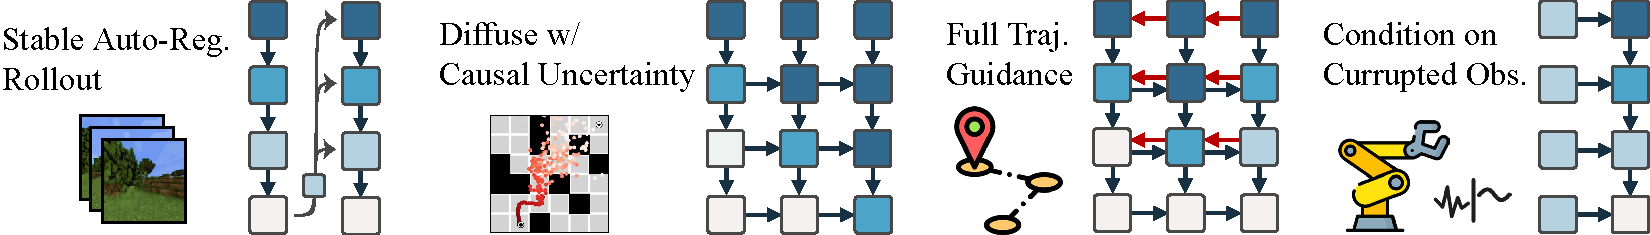
\includegraphics[width=\linewidth]{figures/pdf/Sampling_Schemes.pdf}
    \vspace{-10pt}
\end{figure*}


\paragraph{Stabilizing autoregressive generation.}
\label{par:stabilizing_autoreg}
For high-dimensional, continuous sequences such as video, auto-regressive architectures are known to diverge, especially when sampling past the training horizon.
In contrast, \algo{} can stably  roll out long sequences even beyond the training sequence length by updating the latents using the previous latent associated with  slightly ``noisy tokens'' for some small noise level $0 < k \ll K$. Our experiments (Sec.~\ref{exp:video}) illustrates the resulting marked improvements in long-horizon generation capabilities;  App. \ref{app:noising_long_horizons} provides further intuition.

\paragraph{Keeping the future uncertain.} 
\label{par:zigzag}
Beginning from a sequence of white noise tokens $[\bx^K_1,\bx^K_2,\bx^K_3]^\top$, we may denoise the first token fully and the second token partially, yielding $[\bx^0_1,\bx^{K/2}_2,\bx^K_3]^\top$, then $[\bx^0_1,\bx^{0}_2,\bx^{K/2}_3]^\top$, and finally denoising all tokens fully to $[\bx^0_1,\bx^0_2,\bx^0_3]^\top$. 
Interpreting the noise level as uncertainty, this ``zig-zag'' sampling scheme intuitively encodes the immediate future as more certain than the far future. Sec.~\ref{sec:method_decision_making} describes how this leads to more effective sequence guidance.

\paragraph{Long-horizon Guidance.}
In Line 10 of Algorithm~\ref{alg:diffusion_forcing_sampling}, one may add guidance to the partially diffused trajectory $\bx_{1:T}$ as in Sec.~\ref{sec:related_prelim}. Due to the dependency of future tokens on the past, guidance gradients from future tokens can propagate backwards in time. The unique advantage of \algo{} is that, because we can diffuse future tokens without fully diffusing the past, the gradient guides the sampling of \emph{past} tokens, thereby achieving long-horizon guidance while respecting causality. We elaborate on implementation details in Appendix ~\ref{app:reward_guidance}. As we  show in \Cref{sec:exp_decision_making}, planning in this manner significantly outperforms guided full-sequence diffusion models.

\subsection{\algo{} for Flexible Sequential Decision Making}
\label{sec:method_decision_making}
The capabilities offered by \algo{} motivate our novel framework for sequential decision making (SDM), with key applications to  robotics and autonomous agents. 
Consider a Markov Decision Process defined by an environment with dynamics $ p(\bs_{t+1}|\bs_t, \ba_t)$, observation $ p(\bo_{t}|\bs_t)$ and reward $p(\br_t|\bs_t, \ba_t)$. The goal is to train a policy $\pi(\ba_t|\bo_{1:t})$ such that the expected cumulative reward of a trajectory $\Exp[\sum_{t=1}^{T} \br_t]$ is maximized. 
We assign tokens $\bx_t = [\ba_t, \br_t, \bo_{t+1}]$.  A trajectory is a sequence $\bx_{1:T}$, possibly of variable length;  training is conducted as in Algorithm \ref{alg:diffusion_forcing_training}. 
At each step $t$ of execution, past (noise-free) tokens $\bx_{1:t-1}$ are  summarized by a latent $\bz_{t-1}$.  Conditioned on this latent, we sample, via Algorithm \ref{alg:diffusion_forcing_sampling}, a plan $\hat{\bx}_{t:t+H}$, with $\hat{\bx}_{t}=[\hat{\ba}_t, \hat{\br}_t, \hat{\bo}_{t+1}]^\top$ containing predicted actions, rewards and observations. $H$ is a look-ahead window, analogous to future predictions in model predictive control \cite{garcia1989model}. After taking planned action $\hat{\ba}_t$, the environment produces a reward $\br_t$ and next observation $\bo_{t+1}$, yielding  next token $\bx_t=[\hat{\ba}_t, \br_t, \bo_{t+1}]^\top$. The latent is updated according to the posterior $p_\theta(\bz_{t}|\bz_{t-1}, \bx_t, 0)$. Our framework enables functionality as both \emph{policy} and \emph{planner}:


\paragraph{Flexible planning horizon.} \algons{} (a) can be deployed on \emph{tasks of variable horizon}, because each new action is selected sequentially, and  
(b) its lookahead window $H$ can be shortened to lower latency (using \algo{} as a \emph{policy}), or lengthened to perform long-horizon \emph{planning} (via guidance described below), without re-training or modifications of the architecture. Note that (a) is not possible for full-sequence diffusion models like Diffuser \cite{janner2022planning} with full-trajectory generation horizons, whereas diffusion policies \cite{chi2023diffusion} need fixed, small lookahead sizes, precluding (b). 


\paragraph{Flexible reward guidance.} As detailed in Appendix~\ref{app:reward_guidance},
\algo{} can plan via guidance using any reward (in place of $\log c$) specified over future steps: this includes dense per-time step rewards on the entire trajectory $\sum_{t=1}^T \br_t$, dense rewards on a future lookahead $\sum_{t'=t}^{t+H}\br_t$, and sparse rewards indicating goal completion $-\|\bo_T-\mathbf{g}\|^2$. Per-time step policies cannot take advantage of this latter, longer horizon guidance. 














  



\paragraph{Monte Carlo Guidance (MCG), future uncertainty.}
\algoseq{} allows us to influence the generation of a token $\mathbf{x}_t^k$ by guidance on the whole distribution of future $\mathbf{x}_{t+1:T}$. Instead of drawing a single trajectory sample to calculate this guidance gradient, we can draw multiple samples of the future and average their guidance gradients. We call this Monte Carlo Guidance. In the spirit of so-called shooting methods like MPPI \cite{ williams2015model}, $\mathbf{x}_t^k$ is then guided by the expected reward over the distribution of all future outcomes instead of one particular outcome.  The effect of MCG is enhanced when combined with sampling schedules that keep the noise level of future tokens high when denoising immediate next tokens (e.g. the zig-zag schedule described in Sec.~\ref{par:zigzag}), accounting for greater uncertainty farther into the future. Appendix~\ref{app:cannot_mcg} further justifies the significance of MCG, and why \algo{}  uniquely takes  advantage of it.









\section{Theoretical Properties of Sigmoid Attention}
\label{sec:theory}
We analyze $\sigmoidattn$, with two objectives: (1) showing that a transformer architecture remains a universal function approximator when $\sigmoidattn$ replaces $\softmaxattn$, and (2) recovering a measure of regularity of $\sigmoidattn$ by computing its Lipschitz constant.

\subsection{Are Transformers with Sigmoid Attention Universal Approximators?}
\label{sec:ufa}
\cite{Yun_UAP} demonstrate that classical transformers can approximate continuous sequence-to-sequence functions to arbitrary precision, a property known as the \emph{Universal Approximation Property} (UAP). UAP is highly desirable as it provides proof of an architecture's generalizability and representation capability.
As $\sigmoidattn$ modifies the transformer architecture, it is crucial to theoretically guarantee that this modification does not impact the representation capability and that UAP is retained. We provide this guarantee with the following theorem.
\begin{theorem}[UAP for $\sigmoidattn$]
    \label{thm::UAP}
    We denote with $\mathcal{T}^{h,d_v,r}_{\sigma}$ the class of transformer networks obtainable by combining an arbitrary number of $\sigmoidattn$ layers (each of $h$ heads of dimension $d_v$) followed by FFN layers of hidden dimension $r$.
    For any given continuous, permutation-equivariant function $f:\Omega\subset\mathbb{R}^{n\times d}\to\mathbb{R}^{n\times d}$ with compact support $\Omega$, and for any arbitrarily small error $\varepsilon$, there exists a transformer network $g\in\mathcal{T}_\sigma^{4,1,4}$ such that
    \begin{equation}
        \left(\int_{\Omega}\|f(\bb{X})-g(\bb{X})\|^p_p d\bb{X}\right)\leq\varepsilon,\qquad\text{for}\quad 1\leq p<\infty.
    \end{equation}
\end{theorem}
\Cref{thm::UAP} is the exact counterpart of \cite[Thm.~2]{Yun_UAP}, which shows UAP for classical transformers. Our proof largely follows the same path, an outline of the original proof provided in \cref{app:UAP_proof}. Here, we present an overview of the main adaptations required to prove \cref{thm::UAP} for $\sigmoidattn$, with further details in \cref{sec::proof_modified_sigmoid,sec::proof_contextual_mapping_top}.

\paragraph{Sigmoid Attention layers can implement contextual mappings:} A key step in proving \cref{thm::UAP} is showing that, even with $\sigmoidattn$, a sequence of transformer blocks can implement a \emph{Contextual Mapping} \cite[Def.~3.1]{Yun_UAP}. A contextual mapping characterizes a function that maps each input sequence element to an output \emph{uniquely} dependent on the \emph{whole} sequence. This property allows a transformer to capture and store global context within each token, even if each layer only performs pairwise comparisons. Subsequent layers can then use this global information to map individual tokens to the correct output, ultimately approximating any arbitrary sequence-to-sequence function.

In \cite{Yun_UAP}, the contextual mapping is assembled by modifying individual transformer blocks: each block is tuned to react to a specific input token. By stacking a sequence of these blocks, a transformer can be turned into an accumulator, mapping a given input token sequence to a unique global index. This outcome is achieved via a \emph{selective shift layer} \cite[App.~B.5]{Yun_UAP}:
\begin{equation}
    \Psi(\bb{X};b,b')_{i,1}\coloneqq \begin{cases}
        \max_k \bb{X}_{k,1}-\min_k\bb{X}_{k,1}&\text{if}\quad b<\bb{X}_{i,1}<b'\\
        0&\text{otherwise},
    \end{cases}
    \label{eqn::shift_operation_original}
\end{equation}
and can be approximated using classic attention.
Although $\sigmoidattn$ cannot directly approximate~\cref{eqn::shift_operation_original}, our accumulator definition relies on an equivalent selective shift operation:
\begin{equation}
    \Psi_\sigma(\bb{X};b,b')_{i,1}\coloneqq\begin{cases}
        \sum_{k:\bb{X}_{k,1}> b'} \bb{X}_{k,1} &\text{if}\quad b<\bb{X}_{i,1}<b' \\
        0 &\text{otherwise},
    \end{cases}
    \label{eqn::shift_operation_ours}
\end{equation}
which can be approximated by $\sigmoidattn$ (described in \cref{sec::proof_modified_sigmoid}). In~\cref{sec::proof_contextual_mapping}, we show that~\cref{eqn::shift_operation_ours} shares similar properties with~\cref{eqn::shift_operation_original}, allowing us to use the original proof framework in \cite{Yun_UAP} and demonstrate that UAP holds in our case as well.

Our proof is largely equivalent to that in \cite{Yun_UAP}, with two relevant differences: to approximate \cref{eqn::shift_operation_ours}, we require $\sigmoidattn$ with \textit{at least four heads} and shifts included in both query and key definitions. In contrast, $\softmaxattn$ requires \textit{at least two heads} to approximate~\cref{eqn::shift_operation_original}, with shifts only in the query definition. However, this is primarily a theoretical requirement for the proof and does not affect performance. Notably, the total number of parameters required by both architectures for the approximation follows the same tight scaling of \cite{Yun_UAP}.






\subsection{Regularity of Sigmoid Attention}
\label{sec:regularity}
As with any layer in a neural network, the regularity of $\sigmoidattn$ is important to study, as it gives insights into the robustness of the corresponding network and the ease of optimizing it.
The most standard way to quantify the regularity of a layer function $\phi$ is to compute its \emph{Lipschitz constant} over a set $\mathcal{X}$, that is a constant $C>0$ such that for all $\mX, \mY\in \mathcal{X}$, it holds $\|\phi(\mX) - \phi(\mY)\|\leq C \|\mX - \mY\|$, where $\|\cdot\|$ is the standard Frobenius norm.
The \emph{local} Lipschitz constant is the spectral norm of the Jacobian of $\phi$ at $\mX$.
The two are related: the Lipschitz constant of $\phi$ over $\mathcal{X}$ is the greatest local Lipschitz constant for all $\mX\in \mathcal{X}$.
We turn to the theorem giving the regularity of $\sigmoidattn$:
\begin{theorem}
\label{thm:regularity}
    Define $A = \{\langle \mW_q \vx_i \mW_k \vx_j\rangle|,\enspace i, j\in \{1,\dots,n\}\}\subset\mathbb{R}$ the set of attention weights,  and the scaled activation norms $\sigma_{\infty} = n\times\sup_{u\in A} |\sigma(u)|$ and $\sigma'_{\infty} = n\times \sup_{u\in A} |\sigma'(u)|$.
    Then, the Jacobian of $\sigmoidattn$ at $\mX = (\vx_1, \dots, \vx_n)$ has a spectral norm of at most:
    \begin{equation}
        \|\mW_v\|_2\left(\sigma_{\infty} + 2\sigma'_{\infty} \|\mW_q^T \mW_k\|_2\left(\frac1n\sum_{i=1}^n\|\vx_i\|_2^2\right)\right).
    \end{equation}
\end{theorem}
The proof is found in \cref{app:lipschitz_proof}.
In $\sigmoidattn$, if we assume that the attention weights $\langle \mW_q \vx_i, \mW_k \vx_j\rangle$ are all bounded by a constant $\mu$ --- this is true, e.g., if the activations are bounded --- we get $\sigma_{\infty}\leq \exp(\mu)$ and $\sigma'_{\infty}\leq\exp(\mu)$ thanks to the choice of $b = -\log(n)$.
The bound in \cref{thm:regularity} depends only on the \emph{average} squared-norm of the input sequence $\vx_i$, while classical results for the study of attention all rely on the largest value of $\|\vx_i\|^2_2$~\citep{kim2021lipschitz,castin2023understanding}. 
This is another consequence of the simplicity of sigmoid attention and is due to the removal of the normalizing constant in $\softmaxattn$.
Our result implies that if all $\vx_i$ are within a ball of radius $R$ then the Lipschitz constant of $\sigmoidattn$ grows at most like $R^2$, but it is stronger since we can apply this to unbounded distributions $\vx_i$; it matters only that the second moment is bounded.
This result contrasts sharply with the bounds obtained for $\softmaxattn$: \citet[Thm.~3.4.]{castin2023understanding} show that there exists a sequence $\mX = (\vx_1, \dots, \vx_n)$ with $\|\vx_i\|_2\leq R$ for all $i$ such that the spectral norm of the Jacobian of $\attn$ at $\mX$ is at least $cR^2\exp(cR^2)$ for some constant $c>0$.
On the other hand, our bound scales in $R^2$: this means that the local Lipschitz constant of $\sigmoidattn$ is much lower than the worst local Lipschitz constant of $\softmaxattn$.

\section{Experiments} \label{sec:experiments}


\begin{table*}[t]
% \setlength\tabcolsep{3pt}  %可以控制列间距
% \renewcommand{\arraystretch}{1.1} %可以控制行间距
% \footnotesize
\centering
\fontsize{9}{11}\selectfont
\setlength{\tabcolsep}{2.6mm}{
\begin{tabular}{c|l|cccccc}
\toprule
\multicolumn{1}{c|}{\multirow{2}{*} {Type}} & \multicolumn{1}{l|}{\multirow{2}{*} {Model}}   & \multicolumn{3}{c}{WebQSP}   & \multicolumn{3}{c}{CWQ} \\
\cline{3-8}
 \multicolumn{1}{c|}{} & \multicolumn{1}{c|}{}   &F1&Hits@1& Acc &F1&Hits@1& Acc\\ 
\hline
\hline
\multicolumn{1}{c|}{\multirow{4}{*} {EM-based}} & KV-Mem {\scriptsize \cite{miller2016key}} & 34.5 & 46.7 & - & 15.7 & 18.4 & - \\
\multicolumn{1}{c|}{}& NSM$_{+h}$ {\scriptsize \cite{NSM}} &67.4 & 74.3& - & 44.0& 48.8&-   \\
\multicolumn{1}{c|}{}& TransferNet {\scriptsize \cite{shi2021transfernet}} &-  & 71.4 &- &- &48.6 &  - \\
\multicolumn{1}{c|}{}& KGT5 {\scriptsize \cite{KGT5}} &-  &56.1 &- &- & 36.5&  - \\
\hline
\multicolumn{1}{c|}{\multirow{5}{*} {IR-based}} &  GraftNet {\scriptsize \cite{sun-etal-2018-open}} & 60.4 & 66.4 & - & 32.7 & 36.8 & - \\
\multicolumn{1}{c|}{}& PullNet {\scriptsize \cite{sun-etal-2019-pullnet}} & - & 68.1 & - & - &45.9 & - \\
\multicolumn{1}{c|}{}& SR+NSM {\scriptsize \cite{zhang2022subgraph}} &  64.1 & 68.9 &- &47.1& 50.2&- \\
\multicolumn{1}{c|}{}& SR+NSM+E2E {\scriptsize \cite{zhang2022subgraph}} & 64.1  &69.5 &- &46.3&49.3 &-\\
\multicolumn{1}{c|}{}& UniKGQA {\scriptsize \cite{unikgqa}} & 71.0 &77.0& - &49.4& 50.9 &-\\
\hline
\multicolumn{1}{c|}{\multirow{6}{*} {SP-based}}& CBR-KBQA {\scriptsize \cite{CBR-KBQA}} & 72.8 &- &69.9 &70.0 &-& 67.1 \\
\multicolumn{1}{c|}{}& GMT-KBQA {\scriptsize \cite{GMT-KBQA}} & 76.6 &- &73.1 &77.0 &-& 72.2 \\
\multicolumn{1}{c|}{}& UnifiedSKG {\scriptsize \cite{xie-etal-2022-unifiedskg}} & 73.9 &-& -& 68.8& - &-\\
\multicolumn{1}{c|}{}& RnG-KBQA {\scriptsize \cite{rng-kbqa}} & 75.6&-&-&-&-&-\\
\multicolumn{1}{c|}{}& DecAF {\scriptsize \cite{decaf}} & 78.8&82.1&-&-&70.4&-\\
\multicolumn{1}{c|}{}& FC-KBQA {\scriptsize \cite{fc-kbqa}} & 76.9& - &- &56.4& -& -\\
\hline
\multicolumn{1}{c|}{\multirow{8}{*} {LLM-based}} & KD-CoT {\scriptsize \cite{wang2023knowledge}} & 52.5 & 68.6 & - &-  &55.7 & - \\
\multicolumn{1}{c|}{}& Pangu {\scriptsize \cite{pangu}} & 79.6 & - & - & - & - & - \\
\multicolumn{1}{c|}{}& StructGPT {\scriptsize \cite{structgpt}} & - & 72.6 & -  & -  & - & - \\
\multicolumn{1}{c|}{}& ChatKBQA {\scriptsize \cite{chatkbqa}} & 79.8 &83.2& 73.8 &77.8 &82.7 &73.3\\
\multicolumn{1}{c|}{}& ToG-R (GPT-4) {\scriptsize \cite{TOG}} & - & 82.6 & -  & -  & 69.5 & - \\
\multicolumn{1}{c|}{}& G-Retriever {\scriptsize \cite{G-retriever}} & -& 70.1& -& -& -& -\\
\multicolumn{1}{c|}{}& GNN-RAG {\scriptsize \cite{mavromatis2024gnn}} & 73.5 &82.8& -  &60.4& 62.8& - \\
\rowcolor{gray!10}  \multicolumn{1}{c|}{}& \model (Ours) & \textbf{81.2}\scriptsize{$\pm$0.15} & \textbf{84.3}\scriptsize{$\pm$0.16}  & \textbf{75.2}\scriptsize{$\pm$0.10} & \textbf{78.5}\scriptsize{$\pm$0.11} & \textbf{83.1}\scriptsize{$\pm$0.09} & \textbf{74.5}\scriptsize{$\pm$0.07} \\
\bottomrule
\end{tabular}}
\caption{Performance comparison of different types of KGQA methods on WebQSP and CWQ datasets. We present the Mean scores and standard deviations (mean ± std) of five experiments with different random seeds. The best result is highlighted in \textbf{bold}, and the baseline results are taken from corresponding papers.}
\label{tab:main result}
\end{table*}



\subsection{Experiment Settings}

\textbf{Datasets. }
Our experiments were conducted using two well-known datasets: WebQuestionsSP (WebQSP) \cite{webqsp} and ComplexWebQuestions (CWQ) \cite{CWQ}. The dataset statistics are presented in the Appendix. 
Both datasets contain SPARQL queries that correspond to the questions and can be executed on Freebase to obtain answers.

\noindent\textbf{Baselines.}
In this study, we evaluate performance with 22 baselines, which are categorized into four groups: embedding-based (EM-based), information retrieval-based (IR-based), semantic parsing-based (SP-based), and LLM-based methods. For more detailed descriptions of the baselines, please refer to the Appendix.
It is important to note that some methods, such as DecAF~\cite{decaf}, can be classified as multiple groups, specifically IR-based and SP-based. To ensure fairness, we do not include the results of using the oracle entity linking annotations setting, such as RoG \cite{RoG}. We put the performance comparison of the oracle setting in the Appendix.





\noindent\textbf{Evaluation Metrics.}
We use Hits@1, F1, and Acc as primary evaluation metrics following \cite{chatkbqa}. Hits@1 assesses the accuracy of top-1 predicted answer, F1 considers the coverage of all possible answers, and Acc measures the strict exact-match accuracy.
We further assess the quality of generated S-expressions by employing two metrics: the extract match ratio (EM) and the match after beam search ratio (BM) with ground-truth S-expressions, for analytical experiments.

\noindent\textbf{Implementation Details.}
% We employ LLaMA2-7B and LLaMA2-13B \cite{touvron2023llama} as LLM backbones, and then fine-tune LLMs using LoRA \cite{hu2022lora} on WebQSP and CWQ. 
Following ~\citet{chatkbqa}, we fine-tune LLaMA2-7B on WebQSP and LLaMA2-13B on CWQ using LoRA.
We evaluate the impact of backbones and fine-tuning methods in our subsequent experiments. During inference, we utilize beam search to generate multiple logical forms. We select the executable logical form with the highest score to obtain answers. All experiments were done on NVIDIA A6000 GPUs. We only searched the number of retrievals $k$ with values of \{4,8,16,32,64,100\}. 

\subsection{Main Results}
% In this section, we compare our method with all baselines.
As observed from Table \ref{tab:main result}, \model outperforms all baselines across all metrics on both datasets. Notably, on WebQSP dataset, accuracy has improved by 1.6\% compared to the second-best baseline, ChatKBQA, marking new state-of-the-art performance.
Specifically, \model surpasses subgraph retrieval techniques such as SR+NSM and DecAF with 26\% and 2.4\% F1 improvements on WebQSP, respectively, as well as entity and relation retrieval methods like GMT-KBQA with 5.3\% F1 improvement on WebQSP.
This can be attributed to our proposed self-alignment mechanism, which effectively aligns multi-aspect knowledge.
On the other hand, \model also outperforms other LLM-based approaches, such as G-Retriever and ChatKBQA, suggesting that our approach of learning prompt embeddings for retrieval can more flexibly leverage the capabilities of LLMs to utilize retrieval knowledge.


\begin{table}[t]
\setlength\tabcolsep{2pt}  %可以控制列间距
% \renewcommand{\arraystretch}{1.1} %可以控制行间距
\footnotesize
\centering
\fontsize{9}{11}\selectfont
\setlength{\tabcolsep}{3mm}
\begin{tabular}{l|ccccc}
\toprule
 \multicolumn{1}{l|}{\multirow{2}{*} {Model}} & \multicolumn{5}{c}{WebQSP} \\
\cline{2-6}
 \multicolumn{1}{c|}{} &F1&Hits@1& Acc & EM & BM  \\ 
\hline
\hline
\rowcolor{gray!10} \model & \textbf{81.2} & \textbf{84.3} & \textbf{75.2} & \textbf{63.9} & 76.4\\
w/o \textit{SN} & 80.1 & 83.3 & 74.3& 63.6 & \textbf{77.0}\\
w/o \textit{SA} & 79.5 & 82.6 & 73.8 & 63.0 &75.7 \\
w/o \textit{RG} &79.4 & 82.2 &74.3 & 63.4 & 76.7\\
w/o \textit{SA\&RG} & 78.7& 81.0 & 72.5  & 62.1 & 73.6 \\
w/o \textit{SA\&SN}	&79.1	&82.0	&73.8&	63.1&	76.2\\
w/o \textit{ALL} & 76.2 & 79.5 & 70.1 & 59.7 & 72.4  \\
\bottomrule
\end{tabular}
 \caption{Ablation study of sub-modules on WebQSP dataset.}
\label{tab:ablation}
\end{table}



\subsection{Ablation Study}
In this section, we conduct a series of ablation studies to address the following question: 

\textbf{How do the proposed modules improve performance?} Specifically, we conduct experiments against five variants:
1) w/o \textit{SN}: without siamese network, and relevance score is calculated by vector inner product; 2) w/o \textit{SA}: without self-alignment module; 3)  w/o \textit{RG}: without relevance gating module; 4) w/o \textit{SA\&RG}: without both self-alignment and relevance gating modules, where \model obtains prompt embeddings with only MLP. 5) w/o \textit{ALL}: directly appending the retrieval knowledge as context instead of converting retrieval knowledge to prompt embeddings.
As shown in Table \ref{tab:ablation}, we observe that the performance on most metrics decreases when either \textit{SN}, \textit{SA}, or \textit{RG} is removed. This validates the effectiveness of the proposed sub-modules. Furthermore, we find that performance significantly drops when the entire framework is removed, indicating that appending retrieved knowledge directly as context text introduces a large amount of noise, preventing LLMs from focusing on learning the mapping from question to logical form.
Additionally, we notice that the BM is higher in \model w/o \textit{SN} than in \model. This suggests that the ground-truth logical forms are mostly ranked within the top 2 or lower positions during beam search generation, leading to a lower EM.


\begin{table}[t]
% \setlength\tabcolsep{3pt}  %可以控制列间距
\renewcommand{\arraystretch}{1.1} %可以控制行间距
\footnotesize
\centering
\fontsize{9}{11}\selectfont
\setlength{\tabcolsep}{2.8mm}
\begin{tabular}{l|ccccc}
\toprule
 \multicolumn{1}{l|}{\multirow{2}{*} {Model}} & \multicolumn{5}{c}{WebQSP} \\
\cline{2-6}
 \multicolumn{1}{c|}{} &F1&Hits@1& Acc & EM & BM  \\ 
\hline
\hline
\rowcolor{gray!10} \model & \textbf{81.2} & \textbf{84.3} & \textbf{75.2} & \textbf{63.9} & \textbf{76.4} \\
w/o \textit{Relation} & 78.6 & 81.7 &73.1 & 63.0& 74.9\\
w/o \textit{Entity} & 79.2 & 82.2& 73.5& 63.8 & 74.4\\
w/o \textit{Subgraph} &79.7 &82.9 &73.8 & 63.5 & 75.1 \\
\bottomrule
\end{tabular}
 \caption{Quantitative comparison of the impacts of retrieval information on \model's performance.}
\label{tab:ablation retrieval}
\end{table}


\textbf{What impacts do different aspects of retrieval information have on performance?}
To preserve the integrity of \textsc{Amar}, we remove retrieval knowledge by replacing the text embedding with randomly initialized ones. As shown in Table \ref{tab:ablation retrieval}, the results indicate obvious performance drops after removing retrieval knowledge, including `\textit{subgraph}', `\textit{entity}', and `\textit{relation}'. This decline highlights the significance of different aspects of the retrieval knowledge on the overall performance.
Further analysis reveals that removing the `\textit{relation}' component results in the largest drop in performance, suggesting that `\textit{relation}' plays a crucial role in generating logical expressions. Instead, while the `\textit{subgraph}' still contributes to performance, it appears to be less critical for logical forms than `\textit{relation}' or `\textit{entity}'. These findings provide valuable insights for further optimization of the model.

\subsection{Number of Retrieval Analysis}
In this section, we explore the impact of the number of retrieval knowledge. We compare the approach of directly inputting retrieved data as a \textit{context prompt}. If the input exceeds the maximum context limit (i.e., 4096 for LLaMA2), we truncate the retrieved information from subgraphs. As shown in figure \ref{fig:topk}, it can be observed that when the amount of retrieved data is relatively small, our method does not significantly differ from  \textit{Context Prompt}, which suggests that useful information recalled is still limited.
However, as the quantity of retrieved data increases (e.g., reaching 64 or 100), our method achieves a substantial performance improvement, while \textit{context prompt} drastically declines. This demonstrates that introducing a long context results in substantial noise, making it difficult for LLMs to learn important data.
In contrast, by treating retrieved information as an individual prompt embedding, we avoid the issue of excessively long inputs and better utilize the rich information.



\begin{figure}[t]
\centering
\begin{minipage}[c]{0.225\textwidth}
    \centering
    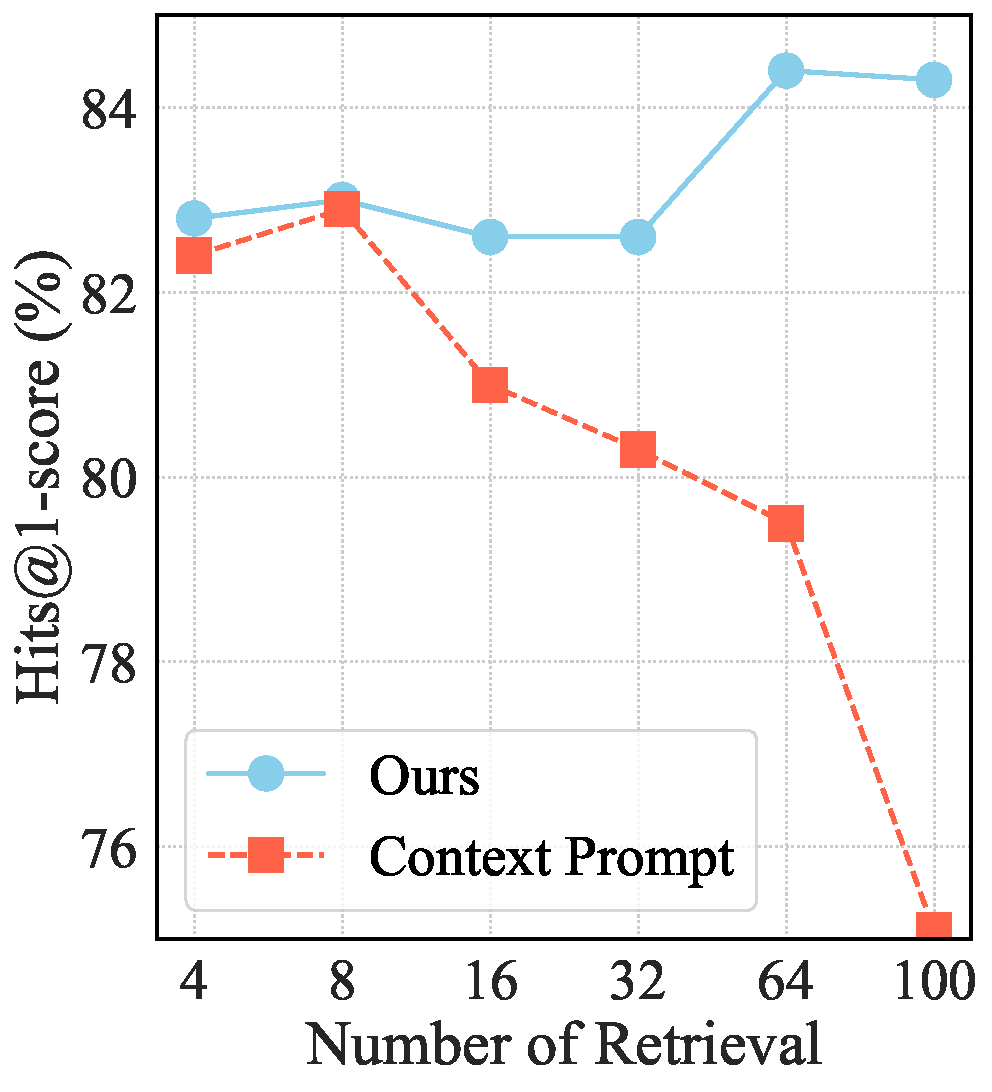
\includegraphics[width=\textwidth]{img/hyperparamter.pdf}
    \caption{Performance vary with the number of Retrieval.}
    \label{fig:topk}
\end{minipage}
\begin{minipage}[c]{0.225\textwidth}
    \centering
    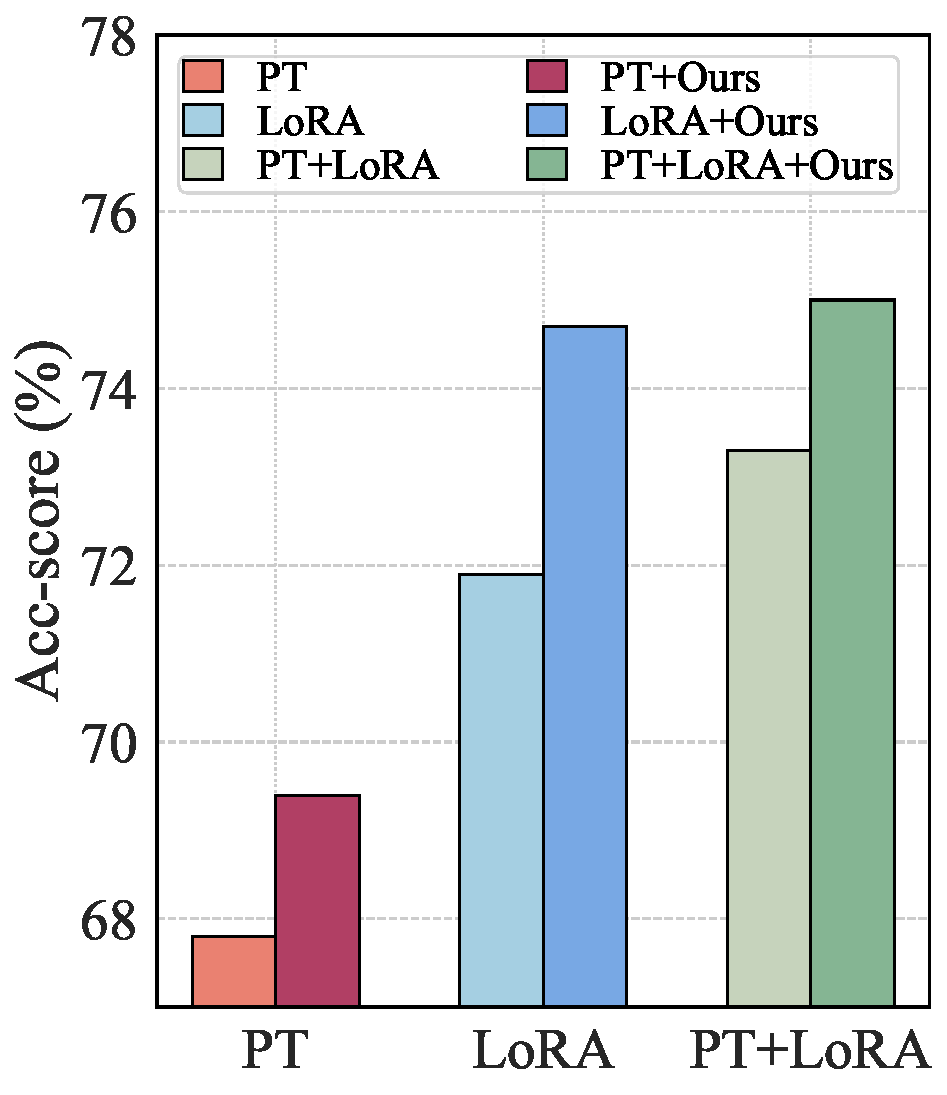
\includegraphics[width=\textwidth]{img/bar.pdf}
    \caption{Combine with different fine-tuning methods.}
    \label{fig:Tuning}
\end{minipage} 
\end{figure}

\begin{table*}[t]
% \setlength\tabcolsep{3pt}  %可以控制列间距
% \renewcommand{\arraystretch}{0.8} %可以控制行间距
\centering
\footnotesize
\begin{tabular}{p{2.7cm}p{14cm}}
\toprule
Question & \textit{what highschool did harper lee go to?} \\
\midrule 
Entity Retrieval & \textit{\ding{172} Harper Lee {[0.9272]}, \ding{173} Senior secondary education {[0.5441]}, 
 \ding{174} Lee Remick {[0.6482]}, \ding{175} Secondary education {[0.5412]}, \ding{176} Barbara Kingsolver {[0.4320]}, \ding{177} High school movement {[0.6758]}}  \\
 \midrule 
Relation Retrieval &  \textit{\ding{172}  people.person.education {[0.9844]},  \ding{173} education.education.institution {[0.9844]},  \ding{174} education.educational\_institution.school\_type {[0.7281]}, \ding{175} education.school.lowest\_grade\_taught {[0.5469]},  \ding{176} education.school\_mascot.school {[0.5431]}, \ding{177} common.topic.notable\_types {[0.8252]}} \\
\midrule 
 Logical Form by \model & \textit{(AND (JOIN common.topic.notable\_types High school) (JOIN (R education.education.institution) (JOIN (R people.person.education) Harper Lee)))} { \CheckmarkBold} \\
\midrule 
 Logical Form by Context Prompt  & \textit{(AND (JOIN \underline{education.educational.institution.school\_type} \underline{School}) (JOIN (R education.education.institution) ( JOIN (R people.person.education) Harper Lee)))} { \XSolidBrush} \\
\bottomrule 
\end{tabular}
\caption{A case study on WebQSP, where the `\textit{[float]}' represents the scores assigned to each retrieval information, indicating the level of influence it has on the model and the \underline{text with underline} means erroneous generation.
}
\label{tab:case}
\end{table*}

\subsection{Efficiency of Fine-Tuning}

In this section, we analyze the efficiency of our method combined with different fine-tuning methods, including Prompt Tuning (PT)~\cite{lester2021prompttuning} and Low-Rank Adaptation (LoRA). To ensure fairness, we conduct fine-tuning experiments without our module by concatenating the retrieved knowledge text with the input context. As shown in Figure \ref{fig:Tuning}, we observe a significant improvement in performance after incorporating \textsc{Amar}, Regardless of whether PT or LoRA is used, our method consistently outperforms baselines.  Notably, the combination of our method with PT+LoRA fine-tuning yields the best results. This highlights the capability of \model to effectively learn from retrieved information, while the direct concatenation of context introduces considerable noise.
Furthermore, we find that LoRA fine-tuning outperforms PT fine-tuning. This can be attributed to the inherent complexity of logical form generation in the KGQA task.  
LoRA has more tunable parameters and can act on all project layers, thus enabling LLMs to better adapt to tasks.


\subsection{Case Study}


In this section, we present a case study to illustrate how our model adaptively learns the importance of retrieval knowledge. We have not presented a case for subgraph retrieval due to its extensive length. As shown in Table \ref{tab:case}, our method is proven effective in assigning high scores to correct entities and relations for entity retrieval and relation retrieval, while irrelevant or misleading information receives low scores. For instance, the entity `\textit{Harper Lee}' received a score of [0.9272], and relation `\textit{people.person.education}' received a score of [0.9844].
Nevertheless, when retrieved text is directly used as the context prompt, it is susceptible to interference from erroneous information in retrieved data. This can result in generating incorrect relations, such as `\textit{education.educational.institution.school type}'. This example highlights that our method not only enhances the performance of LLM in KGQA but also improves the quality of retrieved information by setting weight.

        

\subsection{Analysis of LLM Backbones}
In this section, we investigate the question: \textbf{Does the performance improvement of our method solely come from LLMs?} To answer this, we conduct experiments and compare results using different LLMs as backbones: LLaMA2-7B with fine-tuning, LLaMA2-13B with fine-tuning, and GPT-4 (frozen).
% We observe that when using both LLama2-7b and 13b as backbones, \model outperforms baselines using the same backbone, even better than ToG-R~\cite{TOG} using GPT-4.
In Table \ref{tab:llms}, we observe that \model with LLaMA2-7B and 13B as backbones outperform the baselines using the same backbone, such as ChatKBQA~\cite{chatkbqa}, and both even surpass ToG-R~\cite{TOG} using GPT-4 as the backbone on two datasets.
% Moreover, experiments with LLaMA2-7B even reach slightly better results than with LlaMA2-13B on WebQSP because of over-fitting.
These results suggest that the performance gain of \model is not solely attributed to the use of more capable LLMs but rather to the proposed utilization of the commonality between multi-aspect knowledge and the relevance of the question.
We found that LLaMA2-13B perform worse than LLaMA2-7B on WebQSP. We believe the reason lies in dataset characteristics: the scale of WebQSP (1) is much smaller than that of CWQ, and (2) WebQSP has a maximum complexity, only consisting of 2-hop questions. This may cause the LLaMA2-13B to overfit, leading to reduced performance.


\begin{table}[t]
% \setlength\tabcolsep{3pt}  %可以控制列间距
% \renewcommand{\arraystretch}{1.1} %可以控制行间距
\fontsize{9}{11}\selectfont
\centering
\setlength{\tabcolsep}{3.7mm}{
\begin{tabular}{l|cccc}
\toprule
 \multicolumn{1}{l|}{\multirow{2}{*} {Model}}   & \multicolumn{2}{c}{WebQSP}  & \multicolumn{2}{c}{CWQ}     \\
\cline{2-5}
 \multicolumn{1}{c|}{}   &Acc &Hits@1 &Acc&Hits@1 \\ 
  \hline
  \multicolumn{5}{c}{\textit{GPT-4}} \\
\hline
 ToG-R &- &82.6 &-  & 69.5\\
\hline
\multicolumn{5}{c}{\textit{LLaMA2-7B}} \\
\hline
G-Retriever & - & 70.1& - & - \\
GNN-RAG  &-  & 82.8& -& 62.8\\
ChatKBQA & 73.8 & 83.2 & 73.0 & 82.3 \\
\rowcolor{gray!10}  \model & \textbf{75.2} &\textbf{84.3} & 73.4 & 82.9 \\
 \hline
 \multicolumn{5}{c}{\textit{LLaMA2-13B}} \\
\hline
ChatKBQA & 73.1 & 82.7 & 73.3 & 82.7 \\
\rowcolor{gray!10}  \model & 74.7  &83.3 &\textbf{ 74.5} & \textbf{83.1}\\
\bottomrule
\end{tabular}}
 \caption{Analysis on different LLM backbones. }
\label{tab:llms}
\end{table}



% Answer : Monroe County High School




 

Hyperbolic embeddings embed hierarchical information with high
fidelity and few dimensions. We explored the limits of this approach
by describing scalable, high quality algorithms. We hope the
techniques here encourage more follow-on work on the exciting
techniques of \citet{fb, ucl}. As future work, we hope to explore how
hyperbolic embeddings can be most effectively incorporated into downstream
tasks and applications.


\small\paragraph{Acknowledgements.} This work was supported by the National Science Foundation under Grant No. 2211259, by the Singapore DSTA under DST00OECI20300823 (3D Self-Supervised Learning for Label-Efficient Vision), by the Intelligence Advanced Research Projects Activity (IARPA) via Department of Interior/ Interior Business Center (DOI/IBC) under 140D0423C0075, and by the Amazon Science Hub.



\bibliographystyle{abbrv} 
\bibliography{arxiv}


\newpage
\appendix

\section{Theoretical Justification}
\label{appendix:theory}
\newcommand\numberthis{\addtocounter{equation}{1}\tag{\theequation}}
\newcommand{\cD}{\mathcal{D}}
\newcommand{\unifsim}{\overset{\mathrm{unif}}{\sim}}
\newcommand{\Eforward}{\Exp_{\mathrm{forward}}}
\newcommand{\EforwardD}{\Exp_{\mathrm{forward},\cD}}

\newcommand{\Epz}{\Exp_{p,\mathbf{z}_{1:T}}}
\newcommand{\I}{\mathbf{1}}
\newcommand{\rmd}{\mathrm{d}}
\newcommand{\Dkl}{\mathrm{D}_{\mathbb{KL}}}

\newcommand{\veck}{\mathbf{k}}
\newcommand{\bbK}{\mathbb{K}}
\newcommand{\ptheta}{p_{\bm{\theta}}}

In this section, we provide theoretical justification for the train of \algo. The main contributions can be summarized as follows:
\begin{itemize}
    \item We show that our training methods optimize a reweighting of the Evidence Lower Bound (ELBO) on the average log-likelihood of our data. We first establish this in full generality (\Cref{thm:main_elbo}), and then specialize to the form of Gaussian diffusion (\Cref{cor:elbo}). We show that the resulting terms decouple in such a fashion that, in the limit of a fully expressive latent and model, makes the reweighting terms immaterial. 
    \item We show that the expected likelihood over \emph{any} distribution over sequences of noise levels can be lower bounded by a sum over nonnegative terms which, when reweighted, correspond to the terms optimized in the \algo{} training objective maximizes.  Thus, for a fully expressive network that can drive all terms to their minimal value, \algo{} optimizes a valid surrogate of the likelihood of \emph{all sequences of noise levels simultaneously.}
\end{itemize}

We begin by stating an ELBO for general Markov forward processes $q(\cdot)$, and generative models $\ptheta(\cdot)$, and then specialize to Gaussian diffusion, thereby recovering our loss.  We denote our Markov forward process $q(\cdot)$ as 
\begin{align}
q(\bx^{1:K} \mid \bx^0) = \prod_{k=1}^K q(\bx^k \mid \bx^{k-1}), \label{eq:qforward}
\end{align}
and a parameterized probability model 
\begin{align}
\ptheta(((\bx^{k}_t)_{1 \le k \le K},\bz_t)_{t \ge 1})
\end{align}
We assume that $\ptheta$ satisfies the \emph{Markov property} that 
\begin{align}
&\ptheta(\bz_t, \bx_t^{k_t}\mid \bz_{1:t-1},(\bx_{s}^{k_s})_{1 \le s < t}) = \ptheta(\bz_t, \bx^{k_t}\mid \bz_{t-1})
\end{align} 
that is, the latent codes $\bz_{t-1}$ is a sufficient statistic for $\bx^{k_t}$ given the history. We say that $\ptheta$ has \emph{deterministic latents} if $\ptheta(\bz_t\mid \bz_{1:t-1},(\bx_{s}^{k_s})_{1 \le s < t},\bx_t^{k_t})$ is a Dirac delta. 
\begin{remark} In order for $\ptheta$ to have deterministic latents and correspond to a valid probability distribution, we need to view the latents $\bz_t$ not as individual variables, but as a collection of variables $\bz_t(k_{1:t})$  indexed by $t \in [T]$ and the \emph{history} of noise levels $k_{1:t} \in \{0,1,\dots,K\}^t$. In this case, simply setting $\bz_t(k_{1:t}) = (k_{1:t},(\bx_{s}^{k_s})_{1 \le s \le t}$ tautologically produces deterministic latents. The reason for indexing $\bz_t(k_{1:t})$ with $k_{1:t}$ then arises because, otherwise, $\ptheta(\bz_t \mid ((\bx_{s}^{k_s})_{1 \le s \le t},(\bx_{s}^{k_s'})_{1 \le s \le t})$ would be ill-defined unless $k_s = k_s'$ for all $1 \le s \le t$, and thus, $\ptheta$ would not correspond to a joint probability measure. The exposition and theorem that follows allow $\bz_t(k_{1:t})$ to be indexed on past noise levels $k_{1:t}$ but suppresses dependence on $k_{1:t}$ to avoid notational confusion.
\end{remark}




\subsection{Main Results}
We can now state our main theorem, which provides an evidence lower bound (ELBO) on the expected log-likelihood of partially-noised sequences $(\bx_{t}^{k_t})_{1 \le t \le T}$, under uniformly sampled levels $k_t$ and $\bx_t^{k_t}$ obtained by noising according to $q(\cdot)$ as in \eqref{eq:qforward}. Notice that this formulation does not require an explicit for of $q(\cdot)$ or $\ptheta$, but we will specialize to Gaussian diffusion in the following section. 
\newcommand{\mutheta}{\mu_{\bm{\theta}}}
\begin{theorem}\label{thm:main_elbo}  Fix $\bx_{1:T}^{0}$. Define the expectation over the forward process with random noise level $k_{1:T}$ as 
\begin{align}
\Eforward[\cdot] := \Exp_{k_{1},\dots,k_T \unifsim [K]}\Exp_{\bx_{s}^{k_s}\sim q(\bx_{s}^{k_s} \mid \bx_s^0),1 \le s \le T}[\cdot],
\end{align}
and the expectation over the latents under $\ptheta(\cdot)$ conditioned on $k_{1:T},(\bx_{s}^{k_t})_{1 \le t \le T}$ as 
\begin{align}
\Epz[\cdot] := \Exp_{\bz_{s} \sim p (\bz_{s} \mid \bz_{s-1},\bx_s^{k_s}), s\le T}\left[\cdot \mid k_{1:T}, (\bx_t^{k_t})_{1 \le t \le T}\right]
\end{align}
 Then, as long as $\ptheta$ satisfies the Markov property, 
\begin{align*}
&\Eforward[\ln  \ptheta((\bx_{t}^{k_t})_{1 \le t \le T})] \ge C(\bx_{1:T}^0)  \\
&+ \Eforward\Epz \left[\sum_{t=1}^T \left(\frac{1}{K+1}\ln \ptheta(\bx_t^{0} \mid \bx_{t}^{1},  \bz_{t-1}) +  \sum_{j=2}^{K}\frac{j}{K+1}\Dkl\left(q(\bx_{t}^{j-1} \mid \bx_t^{j},\bx_t^0) \parallel \ptheta(\bx_{t}^{j} \mid \bx_{t}^{j-1}, \bz_{t-1})\right)\right)\right], 
\end{align*}
 where $C(\bx_{1:T}^0)$ is a constant depending only on $\bx_{1:T}^0$ (the unnoised data). Moreover, if the latents are deterministic (i.e. $\ptheta(\bz_t \mid \bz_{t-1},\bx_t^{k_t})$ is a Dirac distribution),  then the inequality holds with inequality if and only if $q(\bx_{t}^{k_t+1:T} \mid \bx_t^{k_t}) \equiv \ptheta(\bx_{t}^{k_t+1:T} \mid \bx_t^{k_t},\bz_{t-1})$, i.e. the variational approximation is exact. 
\end{theorem}
The proof of the above theorem is given in \Cref{sec:proof:thm:main_elbo}. Remarkably, it involves \emph{only two} inequalities! The first holds with equality under deterministic latents and the second holds if and only if variational approximation is exact: $q(\bx_{t}^{k_t+1:T} \mid \bx_t^{k_t}) \equiv \ptheta(\bx_{t}^{k_t+1:T} \mid \bx_t^{k_t},\bz_{t-1})$. This tightness of the ELBO suggests that the expression in \Cref{thm:main_elbo} is a relatively strong surrogate objective for optimizing the likelihoods. 

\subsubsection{Specializing to Gaussian diffusion}
We now special \Cref{thm:main_elbo} to Gaussian diffusion. For now, we focus on the ``$\bx$-prediction'' formulation of diffusion, which is the one used in our implementation. The ``$\beps$-prediction'' formalism, used throughout the main body of the text, can be derived similarly (see Section 2 of \cite{chan2024tutorial} for a clean exposition). The following theorem follows directly by apply standard likelihood and KL-divergence computations for the DDPM \cite{ho2020denoising,chan2024tutorial} to \Cref{thm:main_elbo}.  
\newcommand{\xthet}{\hat{\bx}_{\bm\theta}}
\begin{corollary}\label{cor:elbo} Let 
\begin{align}
q(\bx^{k+1} \mid \bx_t^k) = \mathcal{N}(\bx^k; \sqrt{1-\beta_k}\bx^{k-1}, \beta_k \mathbf{I}),
\end{align}
and define $\alpha_k = (1-\beta_k)$, $\bar{\alpha}_k = \prod_{j=1}^k \alpha_j$.  Suppose that we parameterize $\ptheta(\bx_{t}^{j} \mid \bx_{t}^{j+1},\bz_{t-1}) = \cN(\mutheta(\bx_{t}^{j+1},\bz_{t-1},j),\sigma_j^2)$, where further, 
\begin{align*}
\mutheta(\bx_{t}^{j},\bz_{t-1},j) = \frac{(1 - \bar{\alpha}_{j-1})\sqrt{{\alpha}_j}}{1-\bar{\alpha}_j} \bx_t^j +  \frac{(1 - {\alpha}_{j})\sqrt{\bar{\alpha}_{j-1}}}{1-\bar{\alpha}_j}\xthet(\bx_{t}^{j},\bz_{t-1},j), \quad \sigma_j^2 := \frac{(1 - \alpha_{j})(1-\sqrt{\bar{\alpha}_{j-1}})}{1-\bar{\alpha}_j}.
\end{align*}
 Then, as long as $\ptheta$ satisfies the Markov property, we obtained
\begin{align*}
\Eforward[\ln  \ptheta((\bx_{t}^{k_t})_{1 \le t \le T})] + C(\bx_{1:T}^0)  &\ge \Eforward\Epz \left[\sum_{t=1}^T  \frac{j}{K+1}\sum_{j=1}^{K}c_j \| \hat{\bx}^0_{\bm{\theta}}(\bx_{t}^{j},\bz_{t-1},j) - \bx_t^0\|^2 \right]\\
&= \Eforward\Epz \left[\sum_{t=1}^T  \I\{k_t \ge 1\}\cdot k_tc_{k_t} \| \hat{\bx}^0_{\bm{\theta}}(\bx_{t}^{k_t},\bz_{t-1},{k_t}) - \bx_t^0\|^2 \right],
\end{align*}
where above, we define $c_j = \frac{(1 - \alpha_{j})^2\bar{\alpha}_{j-1}}{2\sigma^2(1 - \bar\alpha_{j})^2}$.
\end{corollary}
\begin{proof} The first inequality follows from the standard computations for the ``$\bx$-prediction'' formulation of Diffusion (see Section 2.7 of  \cite{chan2024tutorial} and references therein). The second follows by replacing the sum over $j$ with an expectation over $k_t \unifsim \{0,1,\dots,K\}$. 
\end{proof}
We make a couple of remarks:
\begin{itemize}
    \item As noted above, \Cref{cor:elbo} can also be stated for $\beps$-prediction, or the so-called ``$\mathbf{v}$-prediction'' formalism, as all are affinely related. 
    \item Define an idealized latent $\tilde{\bz}_{t-1}$ consisting of all past tokens $(\bx_t^{k_t})$ as well as of their noise levels $k_t$. This is a sufficient statistic for $\bz_{t-1}$, and thus we can always view $\hat{\bx}^0_{\bm{\theta}}(\bx_{t}^{k_t},\bz_{t-1},{k_t}) = \hat{\bx}^0_{\bm{\theta}}(\bx_{t}^{k_t},\bar\bz_{t-1},{k_t}) $, where $\bz_{t-1}$ is just compressing $\bar \bz_{t-1}$.  When applying the expectation of $\bx_{1:T} \sim q$ to both sides of the bound in \Cref{cor:elbo}, and taking an infimum over possible function approximator $\hat{\bx}^0_{\theta}$, we obtain
    \begin{align*}
        \inf_{p_\theta} \Exp_{q}\Eforward \Epz \| \hat{\bx}^0_{\bm{\theta}}(\bx_{t}^{k_t},\bz_{t-1},{k_t}) - \bx_t^0\|^2 &= \inf_{p_\theta} \Exp_{q}\Eforward \Epz \| \hat{\bx}^0_{\bm{\theta}}(\bx_{t}^{k_t},\bar{\bz}_{t-1}) - \bx_t^0\|^2 \\
        &= \mathbf{Var}_{q}[\bx_t^0 \mid (\bx_s^{k_s})_{1 \le s \le t}, k_1,\dots,k_t ]. 
    \end{align*}
    This leads to a striking finding: with expressive enough latents and $p_{\theta}$, we can view the maximization of each term in \Cref{cor:elbo} separately across time steps. The absence of this coupling means that the weighting terms are immaterial to the optimization, and thus can be ignored. 
    \item Given the above remarks, we can optimize the ELBO by taking gradients through the objective specified by \Cref{cor:elbo}, and are free to drop any weighting terms (or rescale them) as desired. Backpropagation through $\Epz$ is straightforward due to deterministic latents. This justifies the correctness of our training objective  \eqref{eq:train} and protocol \Cref{alg:diffusion_forcing_training}.
\end{itemize}



\subsubsection{Capturing all subsequences}
\Cref{thm:main_elbo} stipulates that, up to reweighting, the \algo{} objective optimizes a valid ELBO on the expected log-likelihoods over uniformly sampled noise levels.  The following theorem can be obtained by a straightforward modification of the proof of \Cref{thm:main_elbo} generalizes this to arbitrary (possibly temporally correlated) sequences of noise. 




\begin{theorem}\label{thm:main_elbo_general} Let $\cD$ be an arbitrary distribution over $[K]^T$, and define $P_t(j \mid k_{1:t-1}) := \Pr_{\cD}[k_t = j \mid k_{1:t-1}]$.
Fix $\bx_{1:T}^{0}$. Define the expectation over the forward process with random noise level $k_{1:T}$ as 
\begin{align}
\EforwardD[\cdot] := \Exp_{k_{1},\dots,k_T \sim \cD}\Exp_{\bx_{s}^{k_s}\sim q(\bx_{s}^{k_s} \mid \bx_s^0),1 \le s \le T}[\cdot],
\end{align}
and the expectation over the latent under $\ptheta(\cdot)$ conditioned on $k_{1:T},(\bx_{s}^{k_t})_{1 \le t \le T}$ as 
\begin{align}
\Epz[\cdot] := \Exp_{\bz_{s} \sim p (\bz_{s} \mid \bz_{s-1},\bx_s^{k_s}), s\le T}\left[\cdot \mid k_{1:T}, (\bx_t^{k_t})_{1 \le t \le T}\right]
\end{align}
 Then, as long as $\ptheta$ satisfies the Markov property, 
\begin{align*}
&\EforwardD[\ln  \ptheta((\bx_{t}^{k_t})_{1 \le t \le T})] \ge C(\bx_{1:T}^0) +  \EforwardD\Epz \left[\sum_{t=1}^T \Xi_t\right], \text{where } \\
&\Xi_t :=  \left(P_t(1 \mid k_{1:t-1})\ln \ptheta(\bx_t^{0} \mid \bx_{t}^{1},  \bz_{t-1}) +  \sum_{j=2}^{K}j P_t(j \mid k_{1:t-1}) \Dkl\left(q(\bx_{t}^{j-1} \mid \bx_t^{j},\bx_t^0) \parallel \ptheta(\bx_{t}^{j} \mid \bx_{t}^{j-1}, \bz_{t-1})\right)\right), 
\end{align*}
 where $C(\bx_{1:T}^0)$ is a constant depending only on $\bx_{1:T}^0$ (the noise-free data), and where the inequality is an \emph{equality} under the conditions that (a) $\ptheta(\bz_t \mid \bz_{t-1},\bx_t^{k_t})$ is a Dirac distribution (deterministic latents), and (b) $q(\bx_{t}^{k_t+1:T} \mid \bx_t^{k_t}) \equiv \ptheta(\bx_{t}^{k_t+1:T} \mid \bx_t^{k_t},\bz_{t-1})$, i.e. the variational approximation is sharp. 

 In particular, in the Gaussian case of \Cref{cor:elbo}, we have
     \begin{align*}
\EforwardD[\ln  \ptheta((\bx_{t}^{k_t})_{1 \le t \le T})] + C(\bx_{1:T}^0)  
&\ge \EforwardD\Epz \left[\sum_{t=1}^T  \I\{k_t \ge 1\} k_t c_{k_t} \| \hat{\bx}^0_{\bm{\theta}}(\bx_{t}^{k_t},\bz_{t-1},{k_t}) - \bx_t^0\|^2 \right],
\end{align*}

\end{theorem}
The most salient case for us is the restriction of $\cD$ to fixed sequences of noise $k_1,\dots,k_T$ (i.e. Dirac distributions on $[K]^T$). In this case, $P_t(j \mid k_{1:t-1}) = 0$ for all but $j = k_t$, and thus our training objective need not be a lower bound on $\EforwardD[\ln  \ptheta((\bx_{t}^{k_t})_{1 \le t \le T})]$. However, the terms in the lower bound are, up to reweighting, an \emph{subset} of those terms optimized in the training objective. Thus, in light of the remarks following \Cref{cor:elbo}, a fully expressive network can optimize all the terms in the loss simultaneously. We conclude that, for a fully expressive neural network, optimizing the training objective \eqref{eq:train} is a valid surrogate for maximizing the likelihood of all possible noise sequences. 


\subsection{Proof of \Cref{thm:main_elbo}}\label{sec:proof:thm:main_elbo}

Define $\Exp_{< t}[\cdot]$ as shorthand for $\Exp_{k_{1:s}\unifsim [K]}\Exp_{\bx_{s}^{k_s}\sim q(\bx_{s}^{k_s} \mid \bx_s^0),1 \le s \le t-1}\Exp_{\bz_{s} \sim p (\bz_{s} \mid \bz_{s-1},\bx_s^{k_s}), s\le t} [\cdot]$. We begin with the following claim
\begin{claim}[Expanding the latents]\label{claim:first_claim} The following lower bound holds:
\begin{align}
\Eforward[\ln  \ptheta((\bx_{t}^{k_t})_{1 \le t \le T})] &\ge \sum_{t=1}^T \Exp_{<t}\Exp_{k_t \unifsim\{0,1,\dots,K\}}\Exp_{\bx_t^{k_t} \sim q(\bx_t^{k_t} \mid \bx_t^0)}\left[\ln \ptheta(\bx_{t}^{k_t} \mid \bz_{t-1})\right],
\end{align}
Moreover, this lower bound holds with equality if $\bz_{s} \sim p (\bz_{s} \mid \bz_{s-1},\bx_s^{k_s})$ is a Dirac distribution (i.e., deterministic latents).
\end{claim}
\begin{proof}
Let's fix a sequence $k_{1:T}$. It holds that
\begin{align}
\ptheta((\bx_{t}^{k_t})_{1 \le t \le T}) &= \int_{\bz_{1:T} } \prod_{t=1}^T p (\bx_{t}^{k_t}, \bz_{t}\mid (\bx_s^{k_s},\bz_{s})_{s < t}) \nonumber\\
    &= \int_{\bz_{1:T}} \prod_{t=1}^T p (\bx_{t}^{k_t}, \bz_{t}\mid \bz_{t-1}) \tag{Markov Property}\\
    &= \int_{\bz_{1:T}(\veck)} \prod_{t=1}^Tp (\bz_{t} \mid \bz_{t-1},\bx_t^{k_t}) \ptheta(\bx_{t}^{k_t} \mid \bz_{t-1}) \nonumber\\
    &= \Exp_{\bz_{s} \sim p (\bz_{s} \mid \bz_{s-1},\bx_s^{k_s}), s\le T} \prod_{t=1}^T \ptheta(\bx_{t}^{k_t} \mid \bz_{t-1}). \tag{Importance Sampling}
\end{align}
Thus, by Jensen's inequality, 
\begin{align*}
\ln  \ptheta((\bx_{t}^{k_t})_{1 \le t \le T}) &\ge \Exp_{\bz_{s} \sim p (\bz_{s} \mid \bz_{s-1},\bx_s^{k_s}), s\le T} \sum_{t=1}^T \ln \ptheta(\bx_{t}^{k_t} \mid \bz_{t-1}) = \Epz\left[\sum_{t=1}^T \ln \ptheta(\bx_{t}^{k_t} \mid \bz_{t-1})\right],
\end{align*}
where the inequality is and equality when $\ptheta(\bz_s \mid \bz_{s-1},\bx_s^{k_s})$ is a Dirac distribution. By applying $\Eforward$ to both sides of the above display, and invoking the Markov property of the latents, we conclude that
\begin{align*}
\Eforward[\ln  \ptheta((\bx_{t}^{k_t})_{1 \le t \le T})] &\ge \Eforward\Epz\left[\sum_{t=1}^T \ln \ptheta(\bx_{t}^{k_t} \mid \bz_{t-1})\right] \\
&\quad=  \sum_{t=1}^T \Exp_{<t}\Exp_{k_t \unifsim\{0,1,\dots,K\}}\Exp_{\bx_t^{k_t} \sim q(\bx_t^{k_t} \mid \bx_t^0)}\left[\ln \ptheta(\bx_{t}^{k_t} \mid \bz_{t-1})\right].
\end{align*}
\end{proof}
We now unpack the terms obtained from the preceding claim.
\begin{claim}[ELBO w.r.t. $q$]  It holds that
\begin{align*}
\Exp_{\bx_t^{k_t} \sim q(\bx_t^{k_t} \mid \bx_t^0)}\left[\ln \ptheta(\bx_{t}^{k_t} \mid \bz_{t-1})\right] \ge C_1(\bx_0,k_t) + \left[\Exp_{\bx_t^{k_t:K} \sim q(\bx_t^{k_t:K} \mid \bx_t^0)}  \ln\frac{\ptheta(\bx_{t}^{k_t:K} \mid \bz_{t-1})}{q(\bx_t^{k_t+1:K} \mid \bx_t^{0})}\right].
\end{align*}
where $ C_1(\bx_0,k_t) $ is a constant depending only on $\bx_0$ and $k_t$, and where the inequality holds with equality if and only if $q(\bx_{t}^{k_t+1:T} \mid \bx_t^{k_t}) \equiv \ptheta(\bx_{t}^{k_t+1:T} \mid \bx_t^{k_t},\bz_{t-1})$. 
\end{claim}
\begin{proof}
We have that 
\begin{align*}
&\Exp_{\bx_t^{k_t} \sim q(\bx_t^{k_t} \mid \bx_t^0)}\left[\ln \ptheta(\bx_{t}^{k_t} \mid \bz_{t-1})\right]\\
 &= \Exp_{\bx_t^{k_t} \sim q(\bx_t^{k_t} \mid \bx_t^0)} \left[\ln \int  \ptheta(\bx_{t}^{k_t:K} \mid \bz_{t-1})\rmd \bx_{t}^{k_t+1:K}\right]\\
&= \Exp_{\bx_t^{k_t} \sim q(\bx_t^{k_t} \mid \bx_t^0)}\left[\ln\left(\Exp_{\bx_t^{k_t+1:K} \sim q(\bx_t^{k_t+1:K} \mid \bx_t^{k_t})}  \left[\frac{\ptheta(\bx_{t}^{k_t:K} \mid \bz_{t-1})}{q(\bx_t^{k_t+1:K} \mid \bx_t^{k_t})}\right]\right)\right] \\
&\ge \Exp_{\bx_t^{k_t} \sim q(\bx_t^{k_t} \mid \bx_t^0)}\left[\Exp_{\bx_t^{k_t+1:K} \sim q(\bx_t^{k_t+1:K} \mid \bx_t^{k_t})}\left[  \ln\frac{\ptheta(\bx_{t}^{k_t:K} \mid \bz_{t-1})}{q(\bx_t^{k_t+1:K} \mid \bx_t^{k_t})}\right]\right] \tag{(Jensen's inequality)}\\
&= \Exp_{\bx_t^{k_t:K} \sim q(\bx_t^{k_t:K} \mid \bx_t^0)}  \left[\ln\frac{\ptheta(\bx_{t}^{k_t:K} \mid \bz_{t-1})}{q(\bx_t^{k_t+1:K} \mid \bx_t^{k_t})}\right] \tag{Markov property of $q(\cdot)$} \\
&= C_1(\bx_0,k_t) + \left[\Exp_{\bx_t^{k_t:K} \sim q(\bx_t^{k_t:K} \mid \bx_t^0)}  \ln\frac{\ptheta(\bx_{t}^{k_t:K} \mid \bz_{t-1})}{q(\bx_t^{k_t+1:K} \mid \bx_t^{0})}\right],
\end{align*}
where the constant $ C_1(\bx_0,k_t) = \Exp_{\bx_t^{k_t:K} \sim q(\bx_t^{k_t:K} \mid \bx_t^0)}\left[ \ln\frac{q(\bx_t^{k_t+1:K} \mid \bx_t^{0})}{q(\bx_t^{k_t+1:K} \mid \bx_t^{k_t})}\right]$ depends only on $\bx_0$ and $k_t$. To check the conditions for equality, note that if $q(\bx_{t}^{k_t+1:T} \mid \bx_t^{k_t}) \equiv \ptheta(\bx_{t}^{k_t+1:T} \mid \bx_t^{k_t},\bz_{t-1})$, then 
\begin{align*}
\Exp_{\bx_t^{k_t+1:K} \sim q(\bx_t^{k_t+1:K} \mid \bx_t^{k_t})}\left[  \ln\frac{\ptheta(\bx_{t}^{k_t:K} \mid \bz_{t-1})}{q(\bx_t^{k_t+1:K} \mid \bx_t^{k_t})}\right] &=   \ln \ptheta(\bx_{t}^{k_t} \mid \bz_{t-1}) + \Exp_{\bx_t^{k_t+1:K} \sim q(\bx_t^{k_t+1:K} \mid \bx_t^{k_t})}\left[  \ln \ptheta(\bx_{t}^{k_t+1:K} \mid \bz_{t-1}, \bx_t^{k_t})\right]
\end{align*}
Since $\ln(\cdot)$ is strictly concave, $\Exp_{\bx_t^{k_t+1:K} \sim q(\bx_t^{k_t+1:K} \mid \bx_t^{k_t})}\left[  \ln \ptheta(\bx_{t}^{k_t} \mid \bz_{t-1})\right] = 0$ if and only if $\ptheta(\bx_{t}^{k_t+1:K} \mid \bz_{t-1}, \bx_t^{k_t}) = q(\bx_t^{k_t+1:K} \mid \bx_t^{k_t})$. 
\end{proof}
\begin{claim}[Computing the expected ELBO]
\begin{align*}
&\Exp_{\bx_t^{k_t:K} \sim q(\bx_t^{k_t:K} \mid \bx_t^0)} \ln \frac{ \ptheta(\bx_{t}^{k_t:K} \mid \bz_{t-1})}{q(\bx_t^{k_t+1:K} \mid \bx^{0}_t)} \\
&=C_3(\bx_0,k_t) + \I\{k_t = 0\}\ln \ptheta(\bx_t^{0} \mid \bx_{t}^{1},  \bz_{t-1}) +  \sum_{j=1}^{K-1}\I\{j \ge k_t\}\Dkl\left(q(\bx_{t}^{j} \mid \bx_t^{j+1},\bx_t^0) \parallel \ptheta(\bx_{t}^{j} \mid \bx_{t}^{j+1}, \bz_{t-1})\right)\nonumber,
\end{align*}
where $C_2(\bx_0,k_t)$ is some other constant depending on $\bx_0$ and $k_t$.
\end{claim}
\begin{proof}
The proof invokes similar manipulations to the standard ELBO derivation for diffusion, but with a few careful modifications to handle the fact that we only noise to level $k_t$. As is standard, we  require the identity 
\begin{align}
q(\bx_{t}^{j} \mid \bx_t^{j-1},\bx_t^0) = q(\bx_{t}^{j-1} \mid \bx_t^{j},\bx_t^0) \cdot \frac{q(\bx_{t}^{j} \mid \bx_t^0)}{q(\bx_{t}^{j-1} \mid  \bx_t^0)}. \label{eq:time_reversal}
\end{align}
\paragraph{Part 1: Expanding the likelihood ratios}.  Using the above identity, we obtain
\begin{align*}
&\ln \frac{ \ptheta(\bx_{t}^{k_t:K} \mid \bz_{t-1})}{q(\bx_t^{k_t+1:K} \mid \bx^{0}_t)} \\
&= \ln  p (\bx_t^{K} \mid \bz_{t-1}) + \ln \frac{\ptheta(\bx_t^{k_t} \mid \bx_{t}^{k_t+1},\bz_{t-1})}{q(\bx_{t}^{k_t+1} \mid \bx_t^{0})} + \sum_{j=k_{t}+2}^{K}\ln \frac{\ptheta(\bx_{t}^{j-1} \mid \bx_{t}^{j},\bz_{t-1})}{q(\bx_{t}^{j} \mid \bx_t^{j-1},\bx_t^{0})}\\
&\overset{(i)}{=} \ln  p (\bx_t^{K}\mid \bz_{t-1}) + \ln \frac{\ptheta(\bx_t^{k_t} \mid \bx_{t}^{k_t+1},\bz_{t-1})}{q(\bx_{t}^{k_t+1} \mid  \bx_t^{0})} + \sum_{j=k_{t}+2}^{K}\left(\ln \frac{\ptheta(\bx_{t}^{j-1} \mid \bx_{t}^{j},\bz_{t-1})}{q(\bx_{t}^{j-1} \mid \bx_t^{j},\bx_t^{k_t})} + \ln \frac{q(\bx_{t}^{j-1} \mid \bx_t^{0})}{q(\bx_{t}^{j} \mid \bx_t^{0})}\right)\\
&\overset{(ii)}{=} \ln  p (\bx_t^{K}\mid \bz_{t-1}) + \ln \frac{\ptheta(\bx_t^{k_t} \mid \bx_{t}^{k_t+1},  \bz_{t-1})}{q(\bx_{t}^{k_t+1} \mid  \bx_t^{0})} + \ln \frac{q(\bx_{t}^{k_t+1} \mid \bx_t^{k_t})}{q(\bx_{t}^{K} \mid \bx_t^{k_t})} + \sum_{j=k_{t}+1}^{K-1}\ln \frac{\ptheta(\bx_{t}^{j} \mid \bx_{t}^{j+1}, \bz_{t-1})}{q(\bx_{t}^{j} \mid \bx_t^{j+1},\bx_t^0)} \\
&= \frac{\ln  p (\bx_t^{K}\mid \bz_{t-1})}{q(\bx_{t}^{K} \mid \bx_t^{k_t})} + \ln \ptheta(\bx_t^{k_t} \mid \bx_{t}^{k_t+1},  \bz_{t-1})  + \sum_{j=k_{t}+1}^{K-1}\ln \frac{\ptheta(\bx_{t}^{j} \mid \bx_{t}^{j+1}, \bz_{t-1})}{q(\bx_{t}^{j} \mid \bx_t^{j+1},\bx_t^0)} \\
&= \ln (q(\bx_t^{k_t} \mid \bx_{t}^{k_t+1})^{\I\{k_t \ge 1\}})  + 
\ln\frac{  p (\bx_t^{K}\mid \bz_{t-1})}{q(\bx_{t}^{K} \mid \bx_t^{k_t})} + \ln \frac{\ptheta(\bx_t^{k_t} \mid \bx_{t}^{k_t+1},  \bz_{t-1})}{q(\bx_t^{k_t} \mid \bx_{t}^{k_t+1})^{\I\{k_t \ge 1\}}}  + \sum_{j=k_{t}+1}^{K-1}\ln \frac{\ptheta(\bx_{t}^{j} \mid \bx_{t}^{j+1}, \bz_{t-1})}{q(\bx_{t}^{j} \mid \bx_t^{j+1},\bx_t^0)},
\end{align*}
where $(i)$ uses \ref{eq:time_reversal}, $(ii)$ invokes a cancellation in the telescoping sum, and the final display follows from the computation 
\begin{align}
q(\bx_t^{k_t} \mid \bx_{t}^{k_t+1})^{\I\{k_t \ge 1\}} = \begin{cases} 1 & k_t = 0 \\
q(\bx_t^{k_t} \mid \bx_{t}^{k_t+1}) & k_t \ge 1
\end{cases}.
\end{align}
Observe that, because we don't parameterize $p (\bx_t^{K}\mid \bz_{t-1})$,  $\ln (q(\bx_t^{k_t} \mid \bx_{t}^{k_t+1})^{\I\{k_t \ge 1\}})  + 
\frac{\ln  p (\bx_t^{K}\mid \bz_{t-1})}{q(\bx_{t}^{K} \mid \bx_t^{k_t})}$ can be regarded as some constant $C'(\bx_t^{k_t},\bx_t^{k_t+1},\bx_t^K)$. Thus, 
\begin{align}
&\ln \frac{ \ptheta(\bx_{t}^{k_t:K} \mid \bz_{t-1})}{q(\bx_t^{k_t+1:K} \mid \bx^{0}_t)} = C'(\bx_t^{k_t},\bx_t^{k_t+1},\bx_t^K) + \ln \frac{\ptheta(\bx_t^{k_t} \mid \bx_{t}^{k_t+1},  \bz_{t-1})}{q(\bx_t^{k_t} \mid \bx_{t}^{k_t+1})^{\I\{k_t \ge 1\}}}  + \sum_{j=k_{t}+1}^{K-1}\ln \frac{\ptheta(\bx_{t}^{j} \mid \bx_{t}^{j+1}, \bz_{t-1})}{q(\bx_{t}^{j} \mid \bx_t^{j+1},\bx_t^0)} \label{eq:thing2}
\end{align}


\paragraph{Part 2: Taking expecations.} We can now simplify to taking expectations. Observe that 
\begin{align*}
\Exp_{\bx_t^{k_t:K} \sim q(\bx_t^{k_t:K} \mid \bx_t^0)}\ln \frac{\ptheta(\bx_{t}^{j} \mid \bx_{t}^{j+1}, \bz_{t-1})}{q(\bx_{t}^{j} \mid \bx_t^{j+1},\bx_t^0)} = \Dkl\left(q(\bx_{t}^{j} \mid \bx_t^{j+1},\bx_t^0) \parallel \ptheta(\bx_{t}^{j} \mid \bx_{t}^{j+1}, \bz_{t-1})\right),
\end{align*}
and similarly,
\begin{align*}
\Exp_{\bx_t^{k_t:K} \sim q(\bx_t^{k_t:K} \mid \bx_t^0)} \ln \frac{\ptheta(\bx_t^{k_t} \mid \bx_{t}^{k_t+1},  \bz_{t-1})}{q(\bx_t^{k_t} \mid \bx_{t}^{k_t+1})^{\I\{k_t \ge 1\}}}  = \begin{cases} \ln \ptheta(\bx_t^{0} \mid \bx_{t}^{1},  \bz_{t-1}) & k_t = 0 \\
\Dkl\left(q(\bx_{t}^{k_t} \mid \bx_t^{k_t+1},\bx_t^0) \parallel \ptheta(\bx_{t}^{k_t} \mid \bx_{t}^{j+1}, \bz_{t-1})\right) & k_t \ge 1.
\end{cases}
\end{align*}
Finally, $\Exp_{\bx_t^{k_t:K} \sim q(\bx_t^{k_t:K} \mid \bx_t^0)}  C'(\bx_t^{k_t},\bx_t^{k_t+1},\bx_t^K)$ is a constant $C_2(k_t,\bx_0)$ depending only on $k_t,\bx_0$. 
Thus, from \eqref{eq:thing2}
\begin{align}
&\Exp_{\bx_t^{k_t:K} \sim q(\bx_t^{k_t:K} \mid \bx_t^0)} \ln \frac{ \ptheta(\bx_{t}^{k_t:K} \mid \bz_{t-1})}{q(\bx_t^{k_t+1:K} \mid \bx^{0}_t)}\nonumber\\
&= C_2(k_t,\bx_0) + \I\{k_t = 0\}\ln \ptheta(\bx_t^{0} \mid \bx_{t}^{1},  \bz_{t-1}) +  \sum_{j=\max\{1,k_t\}}^{K-1}\Dkl\left(q(\bx_{t}^{j} \mid \bx_t^{j+1},\bx_t^0) \parallel \ptheta(\bx_{t}^{j} \mid \bx_{t}^{j+1}, \bz_{t-1})\right)\nonumber\\
&= C_2(k_t,\bx_0) + \I\{k_t = 0\}\ln \ptheta(\bx_t^{0} \mid \bx_{t}^{1},  \bz_{t-1}) +  \sum_{j=1}^{K-1}\I\{j \ge k_t\}\Dkl\left(q(\bx_{t}^{j} \mid \bx_t^{j+1},\bx_t^0) \parallel \ptheta(\bx_{t}^{j} \mid \bx_{t}^{j+1}, \bz_{t-1})\right)\nonumber.
\end{align}
\end{proof}


\paragraph{Completing the proof of the ELBO.} We are now ready to complete the proof. By combining the previous two claims, we have
\begin{align*}
&\Exp_{\bx_t^{k_t} \sim q(\bx_t^{k_t} \mid \bx_t^0)}\left[\ln \ptheta(\bx_{t}^{k_t} \mid \bz_{t-1})\right] \\
&\quad\ge C_3(\bx_0,k_t) + \I\{k_t = 0\}\ln \ptheta(\bx_t^{0} \mid \bx_{t}^{1},  \bz_{t-1}) +  \sum_{j=1}^{K-1}\I\{j \ge k_t\}\Dkl\left(q(\bx_{t}^{j} \mid \bx_t^{j+1},\bx_t^0) \parallel \ptheta(\bx_{t}^{j} \mid \bx_{t}^{j+1}, \bz_{t-1})\right),
\end{align*}
where $C_3(\bx_0,k_t) = C_1(\bx_0,k_t)+C_2(\bx_0,k_t)$ and where again, the above is an equality when $q(\bx_{t}^{k_t+1:T} \mid \bx_t^{k_t}) \equiv \ptheta(\bx_{t}^{k_t+1:T} \mid \bx_t^{k_t},\bz_{t-1})$. Taking an expectation over $k_t\unifsim\{0,1,\dots,K\}$, we have
\begin{align}
\Exp_{k_t \unifsim\{0,1,\dots,K\}}[\I\{k_t = 0\}] = \frac{1}{K+1}, \quad \Exp_{k_t \unifsim\{0,1,\dots,K\}}\I\{j \ge k_t\} = \frac{j+1}{K+1}.
\end{align}
and consequently,
\begin{align*}
&\Exp_{k_t \unifsim\{0,1,\dots,K\}}\Exp_{\bx_t^{k_t} \sim q(\bx_t^{k_t} \mid \bx_t^0), 1 \le t \le T} \ln \ptheta((\bx_{t}^{k_t})_{1 \le t \le T})\\
&\quad\ge C_4(\bx_t^0) +\frac{1}{K+1}\ln \ptheta(\bx_t^{0} \mid \bx_{t}^{1},  \bz_{t-1}) +  \sum_{j=1}^{K-1}\frac{j+1}{K+1}\Dkl\left(q(\bx_{t}^{j} \mid \bx_t^{j+1},\bx_t^0) \parallel \ptheta(\bx_{t}^{j} \mid \bx_{t}^{j+1}, \bz_{t-1})\right)
\end{align*}
Invoking \Cref{claim:first_claim},
\begin{align*} 
&\Eforward[\ln  \ptheta((\bx_{t}^{k_t})_{1 \le t \le T})] \\
&\ge \sum_{t=1}^T \Exp_{<t}\Exp_{k_t \unifsim\{0,1,\dots,K\}}\Exp_{\bx_t^{k_t} \sim q(\bx_t^{k_t} \mid \bx_t^0)}\left[\ln \ptheta(\bx_{t}^{k_t} \mid \bz_{t-1})\right]\\
&=\sum_{t=1}^T \Exp_{<t} \left[C_4(\bx_t^0) +\frac{1}{K+1}\ln \ptheta(\bx_t^{0} \mid \bx_{t}^{1},  \bz_{t-1}) +  \sum_{j=1}^{K-1}\frac{j+1}{K+1}\Dkl\left(q(\bx_{t}^{j} \mid \bx_t^{j+1},\bx_t^0) \parallel \ptheta(\bx_{t}^{j} \mid \bx_{t}^{j+1}, \bz_{t-1})\right)\right]
\end{align*}
We conclude by observing that $\sum_{t=1}^T \Exp_{<t} \left[C_4(\bx_t^0)\right]$ is a constant $C(\bx_{1:T}^0)$, and that 
\begin{align*}
&\Exp_{<t}\left[\ln \ptheta(\bx_t^{0} \mid \bx_{t}^{1},  \bz_{t-1})\right] = \Eforward \Epz\left[\ln \ptheta(\bx_t^{0} \mid \bx_{t}^{1},  \bz_{t-1})\right]\\
&\Exp_{<t}\left[\Dkl\left(q(\bx_{t}^{j} \mid \bx_t^{j+1},\bx_t^0) \parallel \ptheta(\bx_{t}^{j} \mid \bx_{t}^{j+1}, \bz_{t-1})\right)\right] \\
&= \Eforward \Epz\left[\Dkl\left(q(\bx_{t}^{j} \mid \bx_t^{j+1},\bx_t^0) \parallel \ptheta(\bx_{t}^{j} \mid \bx_{t}^{j+1}, \bz_{t-1})\right)\right],
\end{align*}
since both terms only depend on $k_{1:t-1},(\bx_s^{k_s})_{1 \le s \le t-1}$ and $\bz_{1:t-1}$. We conclude then that 
\begin{align*}
&\Eforward[\ln  \ptheta((\bx_{t}^{k_t})_{1 \le t \le T})] \ge C(\bx_{1:T}^0) \\
&+ \Eforward\Epz \left[\sum_{t=1}^T \left(\frac{1}{K+1}\ln \ptheta(\bx_t^{0} \mid \bx_{t}^{1},  \bz_{t-1}) +  \sum_{j=1}^{K-1}\frac{j+1}{K+1}\Dkl\left(q(\bx_{t}^{j} \mid \bx_t^{j+1},\bx_t^0) \parallel \ptheta(\bx_{t}^{j} \mid \bx_{t}^{j+1}, \bz_{t-1})\right)\right)\right], 
\end{align*}
as needed. Lastly, we recall that the above is an \emph{equality} under the conditions that \newline (a) $\ptheta(\bz_t \mid \bz_{t-1},\bx_t^{k_t})$ is a Dirac distribution, and (b) $q(\bx_{t}^{k_t+1:T} \mid \bx_t^{k_t}) \equiv \ptheta(\bx_{t}^{k_t+1:T} \mid \bx_t^{k_t},\bz_{t-1})$, and we reindex $j \gets j+1$ to ensure consistency with indexing in standard expositions of the diffusion ELBO. 

\qed






 
















\label{app:intuition}
\section{Additional Intuitions and Explainations}
\subsection{Extension to transformer backbone}
\label{app:transformer}
While this paper focuses on a causal implementation of \algo{} with RNNs, it's easy to adopt \algo{} with modern architectures like transformers. One can simply modify a transformer-based sequence diffusion model to train with independent noise levels across tokens and follow the techniques listed in Section \ref{app:snr_derivation}. A strict implementation of causal \algo{} would involve a causal attention mask on the transformer. However, \algo's fractional masking can do something more interesting: Consider the scenario that we use a transformer without a causal mask. We can still implement causality by controlling noise. By labeling the future as full white noise, there is no information leaked into the past tokens. By labeling future tokens as free of noise, we make the model completely non-causal. By labeling the future tokens as noisy, a slight amount of information about the future is provided for the prediction of past tokens. This effectively states that one only needs a non-causal architecture, but controlling fractional noise of the future, to achieve partial or complete causality. These extensions are beyond the scope of this paper, but we already verified their effectiveness and thus provide them as intuitions for future works.

\subsection{The need for independent noise levels}
\label{app:independent_noise}
When training \algo{}, we choose to sample per-token noise level following i.i.d uniform distribution from $[1,2...K]$. One may wonder about the necessity of this choice. Here we discuss the unique abilities of independent noise and the compute overhead added by it. 

The use of independent noise confers a number of special capabilities in our model, including stabilization of autoregressive rollout~\ref{par:stabilizing_autoreg}, modeling causal uncertainty~\ref{par:zigzag}, and removing the need for expensive reconstruction guidance when conditioning on context~\ref{app:cond_replacement}. None of these capabilities can be achieved by full-sequence diffusion. AR-diffusion~\cite{wu2023ar} and Rolling Diffusion~\cite{ruhe2024rolling} can only achieve the first and third one. There are more sampling-time applications such as flexible frame interpolation. Finally, we also saw the practical benefits of using independent noise in hyperparameter tuning. One can simply try different sampling schemes to figure out the most effective one for their applications. All these capabilities only require training the model once with \algo{}. In contrast, any tuning of the sampling scheme would require re-training the model for AR-diffusion and Rolling Diffusion.  

On the other hand, we didn't observe much computing overhead when comparing \algo{} to full-sequence diffusion, as soon as one closely follows our training techniques like~\ref{app:snr_derivation}. The empirical evidence is based on our experiments with an experimental transformer implementation of \algo{} and is thus not fully consistent with the main paper. However, we present the high-level descriptions below for readers interested in more insights: The complexity added by independent noise levels is in the temporal dimension. Therefore, we first adopt a standard technique for video diffusion models - image pre-training, to abstract away the complexity of the image pixels themselves. Then the complexity left is temporal prediction only. We then take the pre-trained image-only model and continue training it on video data. It turns out the sampling result of \algo{} with fewer training steps in this second stage is already better than that of full-sequence diffusion at convergence. We speculate that the better result is due to the same data-augmentation effect described in prior works~\cite{kingma2024understanding}. This shows that the overhead added by independent noise is well-warranted when considering the overall training compute (including image pre-training). 


\subsection{Guidance as planning}
\label{app:reward_guidance}
As stated in Section~\ref{sec:related_prelim}, one can use the gradient of the logarithmic of a classifier $\log c(y|\bx_t^k)$ to guide the sampling process of diffusion model towards samples with a desired attribute $y$. For example, $y$ can refer to the indicator of a success event.  However, we can consider the logarithmic of a more general \emph{energy function} $c(\bx_t^k)$. This has the interpretation as $\Pr(y | \bx_t^k)$, where $\Pr[ y= 1 \mid \bx_t^k] = e^{c(\bx_t^k)}$. Some popular candidate energies include
\begin{align}
    c(\bx_t^k) =\Exp\left[\sum_{t' > t} \br_{'}(\bx_{t'}^{k_{t'}}) \mid \bx_t^{k}\right],  \label{eq:cost_to_go_guidance}
\end{align}
corresponding to a cost-to-go; we can obtain unbiased estimates of this gradient by using cumulative reward $\tilde  c(\bx_t^k) =\sum_{t' > t} \br_{'}(\bx_{t'}^{k_{t'}})$. We can also use goal distance $c = - \|\bx_T^{k_T} - \mathbf{g}\|^2$ as a terminal reward. We provide details about the guidance function deployed in the maze2d planning experiment in Appendix~\ref{app:maze_guidance}.



\subsection{Noising and stabilizing long-horizon generations}\label{app:noising_long_horizons}
\newcommand{\ksmall}{k_{\mathrm{small}}}
Here, we explain in detail how we use noising to stabilize long-horizon generation. At each time $t$, during the denoising, we maintain a latent $\bz_{t-1}^{\ksmall}$ from the previous time step, with $0 < \ksmall \ll K$ corresponding to some small amount of noise. We then do \emph{next token} diffusion to diffuse the token $\bx_t$ across noise levels $\bx_t^{K},\bx_{t}^{K-1},\dots,\bx_t^0$ (corresponding to \Cref{alg:diffusion_forcing_sampling} with horizon $T = 1$, initial latent $\bz_{t-1}^k$, and noise schedule $\cK_{m,1} = m$); this process also produces latents $\bz_t^K,\bz_t^{K-1},\dots,\bz_t^0$ associated with each noise level. From these, we use the latent $\bz_t^{\ksmall}$ to repeat the process. This noised latent can be interpreted as an implementation of conditioning on $\bx_t^{\ksmall}$ in an autoregressive process. In a potential transformer implementation of \algo{} as we discussed in Appendix~\ref{app:transformer}, one can instead run a forward diffusion on a fully diffused token to achieve stabilization. 

It is widely appreciated that adding noise to data ameliorates long-term compounding error in behavior cloning applications \cite{ke2021grasping,laskey2017dart}, and even induces robustness to non-sequential adversarial attacks \cite{cohen2019certified}. In autoregressive video generation, the noised  $\bx_t^{\ksmall}$ is in-distribution for training, because \algo{} trains from noisy past observation in its training objective.
Hence, this method can be interpreted as a special case of the DART algorithm for behavior cloning \cite{laskey2017dart}, where the imitiator (in our case, video generator) is given actions (in our case, next video frames) from noisy observations (in our case, noised previous frames). Somewhat more precisely, because we use both tokens at training time to train \algo, and using slightly noised tokens for autoregression at test time, our approach inherits the theoretical guarantee of the HINT algorithm \cite{block2023provable}.



\subsection{Why Monte Carlo Guidance relies on \algo}
\label{app:cannot_mcg}
Monte Carlo Guidance provides substantial variance reduction in our estimate of cost-to-go guidance \eqref{eq:cost_to_go_guidance}. This technique crucially relies on the ability to roll out future tokens from current ones to use these sample rollouts to get Monte Carlo estimates for gradients. This is not feasible with full-sequence diffusion, because this requires denoising all tokens in tandem; thus, for a given fixed noise level, there is no obvious source of randomness to use for the Monte Carlo estimate. It may be possible to achieve variable horizon via the trick proposed in the following subsection to simulate future rollouts, but to our knowledge, this approach is nonstandard.  



\subsection{Does the replacement technique lead to flexible horizons in full-sequence diffusion?}
\label{app:cond_replacement}
A naive way to obtain flexible horizon generation in full-sequence diffusion is via the ``replacement trick'': consider a full sequence model trained to diffuse $\bx_{1:T}$, which we partition into $\bx_{1:t-1},\bx_{t:T}]$. Having diffused tokens $\bx_{1:t-1}$, we can attempt to denoise tokens of the form $[\tilde \bx_{1:t-1}^{k},\bx_{t:T}^k]$, where we \emph{fix} $\tilde \bx_{1:t-1}^{k} = \bx_{1:t-1}$ to be the previously generated token, and only have score gradients update the remaining $\bx_{t:T}^k$.  One clear disadvantage of this method is inefficiency - one still needs to diffuse the whole sequence even when there is one step left at $t=T-1$. What's more, \cite{ho2022video} points out that this approach of conditioning, named ``conditioning by replacement'', is both mathematically unprincipled and can lead to inconsistency in the generated sequence. The best fix proposed by~\cite{ho2022video} incorporates an additional gradient term with respect to $\bx_{t:T}$ at every diffusion step; this is still an incomplete fix and suffers the computation cost of an extra backward propagation for every sampling step.

\subsection{Further connection to Bayesian filtering}
The core idea of \algo{} can be interpreted as using diffusion to construct an interpolation between prior distribution and posterior distribution of a Bayes filter. Consider the hybrid distribution $p(\bz_t|\bz_{t-1}, \bx_t^k)$. When $k=0$, this hybrid distribution becomes the posterior $p(\bz_t|\bz_{t-1}, \bx_t)$. On the other hand, when $k=K$, the hybrid distribution becomes $p(\bz_t|\bz_{t-1}, \mathbf{n})$ for $ \mathbf{n}\sim \mathcal{N}(0, \mathbf{I})$. Since the independent Gaussian noise term $ \mathbf{n}$ contains no information about $ \bz$, this is exactly the prior distribution $p(\bz_t|\bz_{t-1})$. By varying $k$ between $K$ and $0$, the same neural network can parameterize everything between prior and posterior.

\begin{figure}
    \centering
    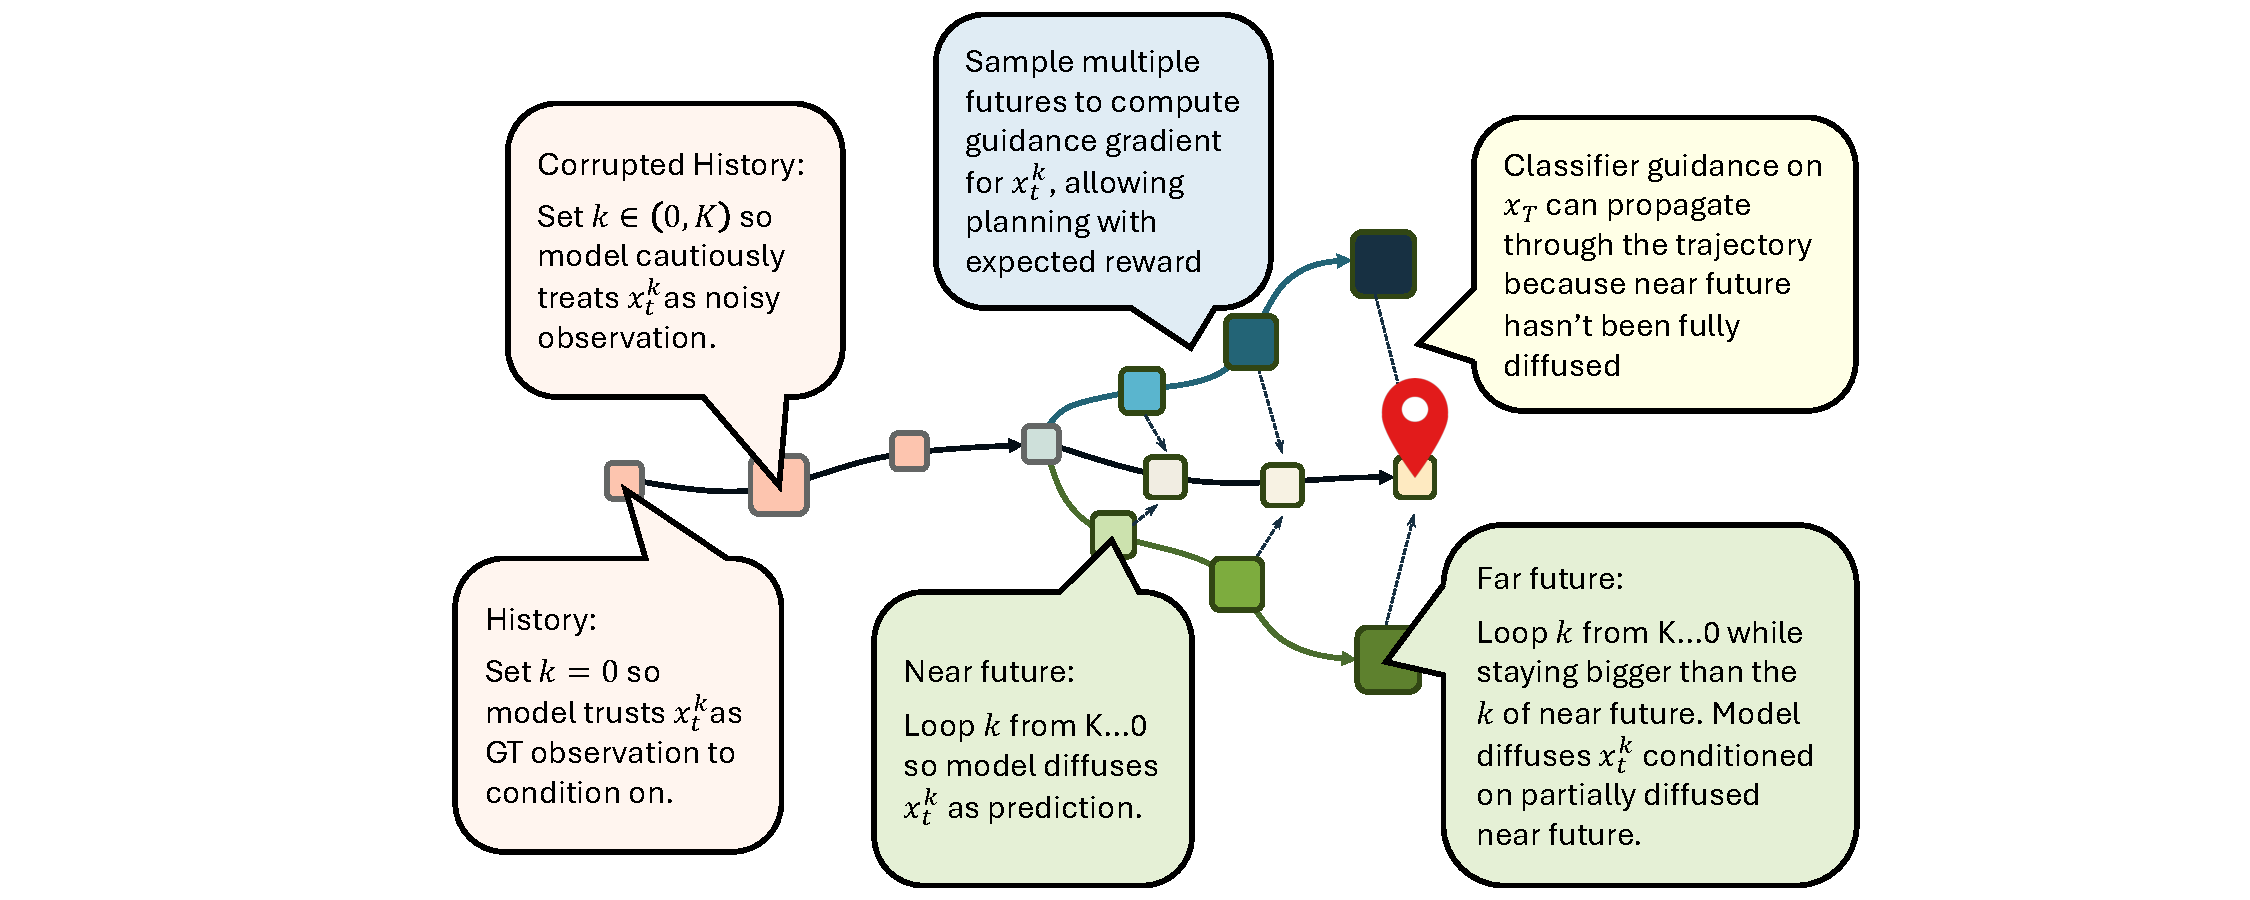
\includegraphics[width=0.8\textwidth]{figures/ability_in_sequence.pdf}
    \caption{\algo{} is trained on independent level of noises at different timesteps. As a result, we can control the noise level $k$ to achieve different effects on conditioning and prediction.}
    \label{fig:ability_in_seq}
\end{figure}

\subsection{Connection to other sequence training schemes}
Noise as masking provides a unified view of different sequence training schemes. The following exposition uses a length $3$ sequence as an example: We always start with fully masked sequence $[\bx_1^K,\bx_2^K,\bx_3^K]$ with the goal of denoising it a ``clean sequence'' of zero noise. $[\bx_1^0,\bx_2^0,\bx_3^0]$. Assume all diffusions are sampled with $3$-step DDIM.

\paragraph{Autoregressive.} In teacher forcing, one trains a model to predict the next token conditioned on prior observations. One can train next-token diffusion models with teacher forcing such as ~\cite{rasul2021autoregressive}: feed neural network with past observations as well as a current observation and ask it to predict clean current observation. A typical training pair can have the input of $[\bx_1^0,\bx_2^0,\bx_3^{K}]^\top$ and target of $[\bx_1^0,\bx_2^0,\bx_3^{0}]^\top$.

At sampling time, one fully diffuses the next token before adding the diffused observation to history to perform an autoregressive rollout. The diffusion process would thus look like 
\begin{align*}
&[\bx_1^K,\bx_2^K,\bx_3^K]^\top\\
&[\bx_1^{K//2},\bx_2^K,\bx_3^K]^\top,\\
&[\bx_1^{0},\bx_2^{K},\bx_3^{K}]^\top,\\
&[\bx_1^{0},\bx_2^{K//2},\bx_3^{K}]^\top\\
&[\bx_1^{0},\bx_2^{0},\bx_3^{K}]^\top,\\
&[\bx_1^{0},\bx_2^{0},\bx_3^{K//2}]^\top,\\
&[\bx_1^{0},\bx_2^{0},\bx_3^{0}]^\top.
\end{align*}
Notably, \algo{} can also perform this sampling scheme at sampling time for applications like imitation learning, when one wants to diffuse the next action as fast as possible.

\paragraph{Full Sequence Diffusion.}
Full sequence diffusion models accept a noisy sequence and denoises level-by-level
\begin{align*}
&[\bx_1^K,\bx_2^K,\bx_3^K]^\top\\
&[\bx_1^{K//2},\bx_2^{K//2},\bx_3^{K//2}]^\top,\\
&[\bx_1^{0},\bx_2^{0},\bx_3^{0}]^\top.
\end{align*}
Notably, \algo{} can also perform this sampling scheme at sampling time.

\paragraph{Diffusion Forcing with causal uncertainty}
As shown in Figure~\ref{fig:method}, to model causal uncertainty, \algo{} keeps the far future more uncertain than the near future by having a larger noise level $k$, at any time of diffusion. An example pattern looks like this:
\begin{align*}
&[\bx_1^K,\bx_2^K,\bx_3^K]^\top\\
&[\bx_1^{K//2},\bx_2^K,\bx_3^K]^\top,\\
&[\bx_1^{0},\bx_2^{K//2},\bx_3^{K}]^\top,\\
&[\bx_1^{0},\bx_2^{0},\bx_3^{K//2}]^\top\\
&[\bx_1^{0},\bx_2^{0},\bx_3^{0}]^\top
\end{align*}
Notable, ~\cite{wu2023ardiffusion} is the first one to propose such a linear uncertainty sampling scheme for causal diffusion models, although \algo{} provides a generalization of such scheme in combination with other abilities.

\paragraph{Diffusion Forcing with stablization}
Previously we introduced the autoregressive sampling scheme that \algo{} can also do. However, such a scheme can accumulate single-step errors because it treats predicted $\bx$ as ground truth observation. \algo{} addresses this problem by telling the model that generated images should be treated as noisy ground truth, as shown in~\ref{fig:method}. 

It first fully diffuses the first token, 
\begin{align*}
&[\bx_1^K,\bx_2^K,\bx_3^K]^\top\\
&[\bx_1^{K//2},\bx_2^K,\bx_3^K]^\top,\\
&[\bx_1^{0},\bx_2^{K},\bx_3^{K}]^\top\\
\end{align*}
Then, it feed the diffused $\bx_1^0$ into the model but tell it is of a slightly higher noise level, as $\bx_1^{1}$ to diffuse $\bx_2$.
\begin{align*}
&[\bx_1^{1},\bx_2^{K//2},\bx_3^{K}]^\top\\
&[\bx_1^{1},\bx_2^{0},\bx_3^{K}]^\top
\end{align*}
Then, it feeds the diffused $\bx_2^0$ into the model but tells it is of a higher noise level, as $\bx_2^{1}$.
\begin{align*}
&[\bx_1^{1},\bx_2^{1},\bx_3^{K//2}]^\top,\\
&[\bx_1^{1},\bx_2^{1},\bx_3^{0}]^\top.
\end{align*}


\section{Extended Related Work}\label{app:extended_related}


\paragraph{Reconstructing masked tokens.} Masked Autoencoders for images~\cite{he2022masked} and videos~\cite{feichtenhofer2022masked} are a popular method for representation learning in pixel space. They have been extended to perform diffusion to generate masked patches conditioned on unmasked ones~\cite{wei2023diffusion,gao2023masked}.

\paragraph{Casting Image Generation as Sequence Generation.} \cite{van2016conditional,chen2020generative} show that even generative modeling of non-sequential data, such as images, can be fruitfully cast as sequence generative modeling.

\paragraph{Non-Diffusion Probabilistic Sequence Models.}
\cite{chung2015recurrent} parameterize token-to-token transitions via a variational auto-encoder. This makes them probabilistic, but does not directly maximize the joint probability of sequences, but rather, enables sampling from the distribution of single-step transitions.

\paragraph{Sequence Diffusion with Varying Noise Levels.} Most similar to our work is AR-Diffusion~\cite{wu2023ardiffusion} which similarly aims to train next-token prediction models for sequence diffusion. Key differences are that AR-Diffusion proposes a noise level that is \emph{linearly} dependent on the position of each word in the sequence, while our critical contribution is to have each noise level be \emph{independent}, as this uniquely enables our proposed sampling schemes, such as stabilizing auto-regressive generation and conditioning on corrupted observations. Further, AR-Diffusion only explores language modeling and does not explore guidance, while we investigate Diffusion Forcing as a broadly applicable sequence generative model with particular applications to sequential decision-making. In particular, we introduce Monte-Carlo Guidance as a novel guidance mechanism. Another closely related work is Rolling Diffusion \cite{ruhe2024rolling}, which proposes to diffuse a sequence with near future more certain and far future more uncertain, resembling the causally uncertain sampling scheme of \algo. Like AR-Diffussion, Rolling Diffusion's training noise levels are linearly dependent on the positions of tokens and must use the exact same noise level scheme at sampling time. It, therefore, shares the aforementioned limitations of AR-Diffusion as well.

\section{Method details}
\label{sec:method_details}

Since we have described the forward pass in~\cref{sec:method}, we describe here
the backward pass in details.

\subsection{Backward Pass}
We show how to compute the backward pass in a fused kernel.


Let $y = f \ast u + \vD u$.
In our case, we have $f$ and $u$ have the same length, so they are symmetric as far as the convolution is concerned.

Suppose we are given $dy = \frac{\partial l}{\partial y}$ (where $l$ is some loss function).
We wish to compute $du$, $df$, and $dD$ (which are $\frac{\partial l}{\partial u}$, $\frac{\partial l}{\partial f}$, and $\frac{\partial l}{\partial \vD}$, respectively).

The most challenging part is computing the gradient through the convolution operator - but we'll see that we can re-use our FFT infrastructure for it.
The rest of the operations are straightforward; we have $d\vD = dy u^T$.

\paragraph{Gradient of the Convolution}

Here, we'll discuss how to compute $df$ by integrating w.r.t. the convolution operator $\ast$.
As an immediate consequence, we'll be able to compute $du$ as well.

Since $f$ and $u$ are the same length $L$, $f \ast u$ and $u \ast f$ have the same result.
%  (this is also clear from the FFT convolution rule, since multiplication is commutative).
Thus, we'll start from $u \ast f$ here.

For some notation, let $O = u \ast f$.
Then, $dO = dy$.
Recall that $O[i] = \sum_{j=0}^{i-1} u[i-j]f[j]$.

We'll start by extending $u$ and $f$ with zeros, to give them length $2L$.
Let $u' = [u[0], u[1], \dots, u[L-1], 0, \dots, 0]$, and $f'$ extended similarly.
Let $O' = u' \ast f'$, and $O = O'[:N]$.
Assume that we have all the values of $dO'$ (we only have them for the first half, but we'll see that it doesn't matter in the end).

Let's construct a Toeplitz matrix $H_{u'}$ such that $u' \ast f' = H_{u'} f'$:
$$
H_{u'} = \begin{bmatrix}
  u'[0] & 0     & \dots & 0 \\
  u'[1] & u'[0] & \dots & 0 \\
  \vdots & \vdots & \ddots & \vdots \\
  u'[2L-1] & u'[2L-2] & \dots & u'[0]
\end{bmatrix}
$$
Since, we have $u'[i] = f'[i] = 0$ for $i \geq L$, we can actually fill in the zeros of the above matrix as well:
$$
H_{u'} = \begin{bmatrix}
  u'[0] & u'[2L-1] & \dots & u'[1] \\
  u'[1] & u'[0] & \dots & u'[2] \\
  \vdots & \vdots & \ddots & \vdots \\
  u'[2L-1] & u'[2L-2] & \dots & u'[0]
\end{bmatrix}
$$
Then, we can use the matrix multiplication chain rule to find that:
\begin{align*}
df' = H_{u'}^T dO' &= \begin{bmatrix}
  u'[0] & u'[1] & \dots & u'[2L-1] \\
  u'[2L-1] & u'[0] & \dots & u'[2L-2] \\
  \vdots & \vdots & \ddots & \vdots \\
  u'[1] & u'[2] & \dots & u'[0]
\end{bmatrix} \\
&= \begin{bmatrix}
  u'[0] & u'[-(2L-1)] & \dots & u'[-1] \\
  u'[-1] & u'[0] & \dots & u'[-2] \\
  \vdots & \vdots & \ddots & \vdots \\
  u'[-(2L-1)] & u'[-(2L-2)] & \dots & u'[0]
\end{bmatrix},
\end{align*}
where we use $u'[-i]$ to mean $u'[2L - i]$.
Notice that this matrix has the same format as $H_{u'}$!
Let $u_*' = [u'[0], u'[-1], \dots, u'[-(2N-1)]]$.
Then:
$$
df' = (u_*' \ast dO').
$$
So how do we compute $u_*'$ efficiently?
Naively, we might incur some nasty memory access issues.
But a nice property about the DFT saves us!

Let $U[i]$ be the $i$-th element of the DFT of a signal $u$.
Note that $U[i]$ is complex.
We have:
$$
U^*[i] = U[-i],
$$
where here the $*$ represents the complex conjugate.
We can use this property to compute $df'$ efficiently:
$$df' = u_*' \ast dO'= iFFT(FFT^*(u')FFT(dO')) \Rightarrow df = df'[:N] = iFFT(FFT^*(u')FFT(dy'))[:N],$$
where $FFT^*$ denotes taking the complex conjugate of the FFT, and $dy'$ denotes $dy$, padded with zeros.

\paragraph{Computing $du$}
We can use this same trick to compute $du$, except we need to add in the contribution from the original $\vD u$ term.
We end up with:
$$du = du'[:N] + \vD dy = iFFT(FFT^*(f')FFT(dy'))[:N] + \vD dy.$$

\subsection{State-Passing Matrices}
\label{sec:state-passing-matrices}

We show how to derive $\vM_{ux}$ for the state update in our state-passing algorithm.

We wish to construct a matrix $vM_{ux} \in \mathbb{R}^{m \times N'}$ such that $\vM_{ux}u = \sum_{i=1}^{N'} \vA^{N'-1}\vB u_i$.
Note that $\vA^i \vB \in \mathbb{R}^{d \times 1}$ is a column vector.
We can simply stack these column vectors to form a matrix:
$\vM_{ux} = [\vA^{N'-1}\vB, \vA^{N'-2}\vB, \dots, \vB]$.
%%% Local Variables:
%%% mode: latex
%%% TeX-master: "../main"
%%% End:


\section{Additional Experiment Results }
\label{app:exp_timeseries}
\subsection{Multivariate Probabilistic Time Series Forecasting} \label{appendix:ts}

\begin{figure}
    \centering
    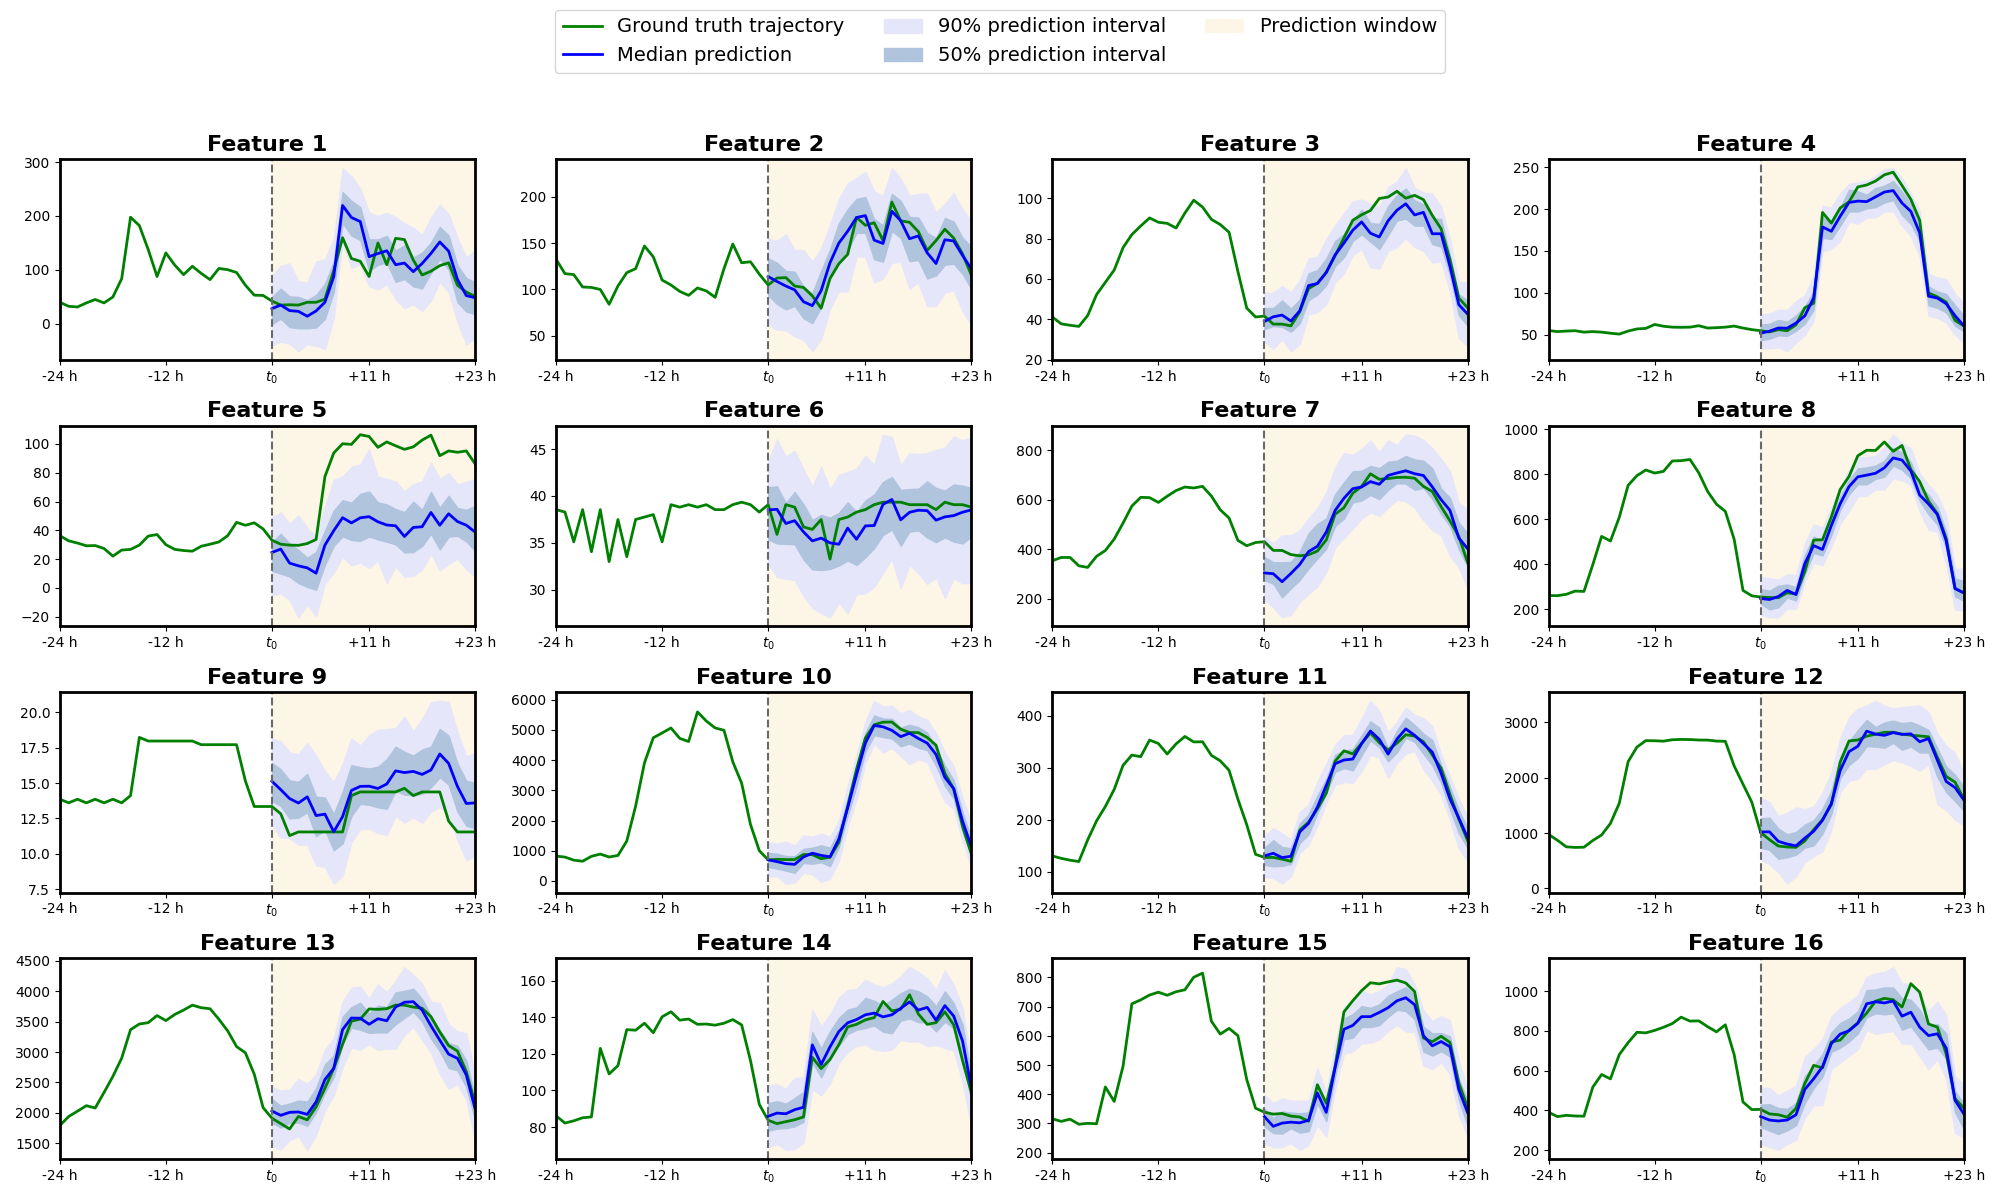
\includegraphics[width=\textwidth]{figures/ts_electricity.png}
    \caption{Prediction intervals of \algo{} for the first prediction window of the test set in the Electricity time series dataset. Only the first 16 features out of 370 are plotted.}
    \label{fig:ts_results}
\end{figure}
To illustrate \algo's new training objective does not degrade it as a generic sequence model, we evaluate \algo{} on high-dimensional and long-horizon sequence prediction tasks in time series prediction. We adopt multiple time series datasets with real-world applications from GluonTS~\cite{gluonts} and evaluate \algo{} with strong baselines with standard metrics in this domain. In this section, we mainly focus on the results and analysis. For a detailed description of datasets and the metric, we refer the reader to Appendix~\ref{app:dataset_timeseries}.

\paragraph{Problem Formulation}
Let $\boldsymbol{X} = \left\{ \mathbf{x}_t \right\}_{t=1}^T$ be a sequence (multivariate time series) of $D$-dimensional observations $\mathbf{x}_t \in \mathbb{R}^D$ of some underlying dynamical process, sampled in discrete time steps $t \in \left\{1, \dots, T\right\}$, where $T \in \mathbb{N}$. In the problem setting of probabilistic time series forecasting, the sequence $\boldsymbol{X} = \left\{ \boldsymbol{X}_c, \boldsymbol{X}_p \right\}$ is split into two subsequences at time step $t_0 \in \mathbb{N}$ with $1 < t_0 \leq T$: the context window $\boldsymbol{X}_c := \left\{ \mathbf{x}_t \right\}_{t=1}^{t_0-1}$ (also called history or evidence) of length $t_0-1$, and the prediction window $\boldsymbol{X}_p := \left\{ \mathbf{x}_t \right\}_{t=t_0}^{T}$ of length~$T - t_0 + 1$ (also known as the prediction horizon). Then, the task is to model the conditional joint probability distribution
\begin{equation} \label{eq:prediction_pdf}
    q{\left( \mathbf{x}_{t_0:T} \mid \mathbf{x}_{1:t_0-1} \right)} := \prod_{t=t_0}^T{q{\left( \mathbf{x}_t \mid \mathbf{x}_{1:t-1} \right)}}
\end{equation}
over the samples in the prediction window. If we know the distribution in~\eqref{eq:prediction_pdf}, we can sample forecast prediction sequences given some initial context from the evidence sequence. However, most time-dependent data generation processes in nature have complex dynamics and no tractable formulation of $q{\left( \mathbf{x}_{t_0:T} \mid \mathbf{x}_{1:t_0-1} \right)}$. Instead, we construct a statistical model that approximates the generative process in~\eqref{eq:prediction_pdf} and estimates quantiles via Monte Carlo sampling of simulated trajectories. In this way, confidence levels or uncertainty measures can be calculated, and point forecasts can be produced as the mean or median trajectory~\cite{hyndman2008forecasting}.

\paragraph{Results.}

\ctable[
    caption = {Results for time series forecasting. We report the test set $\text{CRPS}_\textbf{sum}$ (the lower, the better) of comparable methods on six time series datasets. We measure the mean and standard deviation of our method from five runs trained with different seeds.},
    label = {tab:results_ts},
    pos = ht,
    doinside = \scriptsize,
    center,
    star
]{lccccccc}{}{
    \FL
     Method & Exchange & Solar & Electricity & Traffic & Taxi & Wikipedia
    \ML
    VES~\cite{hyndman2008forecasting} & 0.005 $\pm$ 0.000 & 0.900 $\pm$ 0.003 & 0.880 $\pm$ 0.004 & 0.350 $\pm$ 0.002 & - & - \NN
    VAR~\cite{luetkepohl2007new} & 0.005 $\pm$ 0.000 & 0.830 $\pm$ 0.006 & 0.039 $\pm$ 0.001 & 0.290 $\pm$ 0.001 & - & - \NN
    VAR-Lasso~\cite{luetkepohl2007new} & 0.012 $\pm$ 0.000 & 0.510 $\pm$ 0.006 & 0.025 $\pm$ 0.000 & 0.150 $\pm$ 0.002 & - & 3.100 $\pm$ 0.004 \NN
    GARCH~\cite{weide2002garch} & 0.023 $\pm$ 0.000 & 0.880 $\pm$ 0.002 & 0.190 $\pm$ 0.001 & 0.370 $\pm$ 0.001 & - & - \NN
    DeepAR~\cite{salinas2020deepar} & - & 0.336 $\pm$ 0.014 & 0.023 $\pm$ 0.001 & 0.055 $\pm$ 0.003 & - & 0.127 $\pm$ 0.042 \NN
    LSTM-Copula~\cite{salinas2019highdimensional} & 0.007 $\pm$ 0.000 & 0.319 $\pm$ 0.011 & 0.064 $\pm$ 0.008 & 0.103 $\pm$ 0.006 & 0.326 $\pm$ 0.007 & 0.241 $\pm$ 0.033 \NN
    GP-Copula~\cite{salinas2019highdimensional} & 0.007 $\pm$ 0.000 & 0.337 $\pm$ 0.024 & 0.025 $\pm$ 0.002 & 0.078 $\pm$ 0.002 & 0.208 $\pm$ 0.183 & 0.086 $\pm$ 0.004 \NN
    KVAE~\cite{krishnan2016structured} & 0.014 $\pm$ 0.002 & 0.340 $\pm$ 0.025 & 0.051 $\pm$ 0.019 & 0.100 $\pm$ 0.005 & - & 0.095 $\pm$ 0.012 \NN
    NKF~\cite{bezenac2020normalizing} & - & 0.320 $\pm$ 0.020 & 0.016 $\pm$ 0.001 & 0.100 $\pm$ 0.002 & - & 0.071 $\pm$ 0.002 \NN
    Transformer-MAF~\cite{rasul2021multivariate} & 0.005 $\pm$ 0.003 & 0.301 $\pm$ 0.014 & 0.021 $\pm$ 0.000 & 0.056 $\pm$ 0.001 & 0.179 $\pm$ 0.002 & 0.063 $\pm$ 0.003 \NN
    TimeGrad~\cite{rasul2021autoregressive} & 0.006 $\pm$ 0.001 & 0.287 $\pm$ 0.020 & 0.021 $\pm$ 0.001 & {0.044} $\pm$ {0.006} & 0.114 $\pm$ 0.020 & 0.049 $\pm$ 0.002 \NN
    ScoreGrad sub-VP SDE~\cite{yan2021scoregrad} & 0.006 $\pm$ 0.001 & \textbf{0.256} $\pm$ \textbf{0.015} & \textbf{0.019} $\pm$ \textbf{0.001} & 0.041 $\pm$ 0.004 & {0.101} $\pm$ {0.004} & \textbf{0.043} $\pm$ \textbf{0.002} \NN
    \textbf{Ours} & \textbf{0.003} $\pm$ \textbf{0.001} & {0.289} $\pm$ {0.002} & {0.023} $\pm$ {0.001} & \textbf{0.040} $\pm$ \textbf{0.004} & \textbf{0.075} $\pm$ \textbf{0.002} & 0.085 $\pm$ 0.007
    \LL
}

We evaluate the effectiveness of \algo{} as a sequence model on the canonical task of multivariate time series forecasting by following the experiment setup of ~\cite{salinas2019highdimensional, rasul2021multivariate, rasul2021autoregressive, tang2021probabilistic, yan2021scoregrad}
Concretely, we benchmark \algo{} on the datasets Solar, Electricity, Traffic, Taxi, and Wikipedia. These datasets have different dimensionality, domains, and sampling frequencies, and capture seasonal patterns of different lengths. The features of each dataset are detailed in Table~\ref{tab:ts_data}. We access the datasets from GluonTS~\cite{gluonts}, and set the context and prediction windows to the same length for each dataset. Additionally, we employ the same covariates as~\cite{rasul2021autoregressive}.
We evaluate the performance of the model quantitatively by estimating the Summed Continuous Ranked Probability Score $\operatorname{CRPS}_\text{sum}$ via quantiles. As a metric, $\operatorname{CRPS}_\text{sum}$ measures how well a forecast distribution matches the ground truth distribution.  We provide detailed descriptions of the metric in Appendix~\ref{app:dataset_timeseries}.
We benchmark with other diffusion-based methods in time series forecastings, such as TimeGrad~\cite{rasul2021autoregressive} and the transformer-based Transformer-MAF~\cite{rasul2021multivariate}. In particular, the main baseline of interest, TimeGrad~\cite{rasul2021autoregressive}, is a next-token diffusion sequence model trained with teacher forcing.
We track the $\operatorname{CRPS}_\text{sum}$ metric on the validation set and use early stopping when the metric has not improved for 6 consecutive epochs, while all epochs are fixed to 100 batches across datasets. We then measure the $\operatorname{CRPS}_\text{sum}$ on the test set at the end of the training, which we report in Table~\ref{tab:results_ts}. We use the exact same architecture and hyperparameters for all time series datasets and experiments.
\algo{} outperforms all prior methods except for ~\cite{yan2021scoregrad} with which Diffusion Forcing is overall tied, except for the Wikipedia dataset, on which Diffusion Forcing takes fourth place. 
Note that time series is not the core application of \algo{}, and that we merely seek to demonstrate that the Diffusion Forcing objective is applicable to diverse domains with no apparent trade-off in performance over baseline objectives. 

\subsection{Additional results in compositional generation}
\label{app:exp_compositionality}
Since \algo{} models the joint distribution of any subset of a sequence, we can leverage this unique property to achieve compositional behavior - i.e., \algo{} can sample from the distribution of \emph{subsets} of the trajectory and compose these sub-trajectories into new trajectories. 

In particular, we show that we can also have flexible control over how compositional \algo{} is. As shown in \ref{fig:compositionality}, consider a dataset of trajectories on a 2D, square plane, where all trajectories start from one corner and end up in the opposite corner, forming a cross shape. When no compositional behavior is desired, one can let the models replicate the cross-shaped distribution by allowing full memory of the HMM model. 
When one desires compositional such as generating a V-shaped trajectory, which stitches two sub-trajectories together, one can let the model generate shorter plans with no-memory context using MPC. (Add figures).

\begin{figure}[h]
    \centering
    \begin{subfigure}[t]{.3\linewidth}
        \centering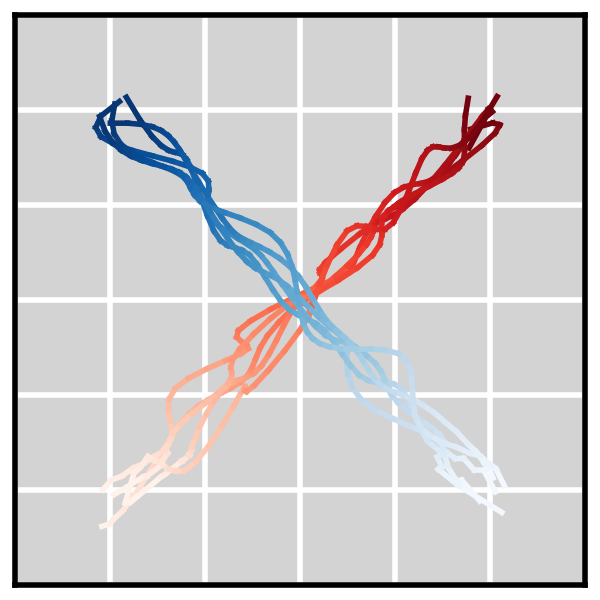
\includegraphics[width=\linewidth]{figures/dataset_diagonal2d_thick_v3.png}
        \caption{Dataset} \label{fig:compositionality_dataset}
    \end{subfigure}
    \begin{subfigure}[t]{.3\linewidth}
        \centering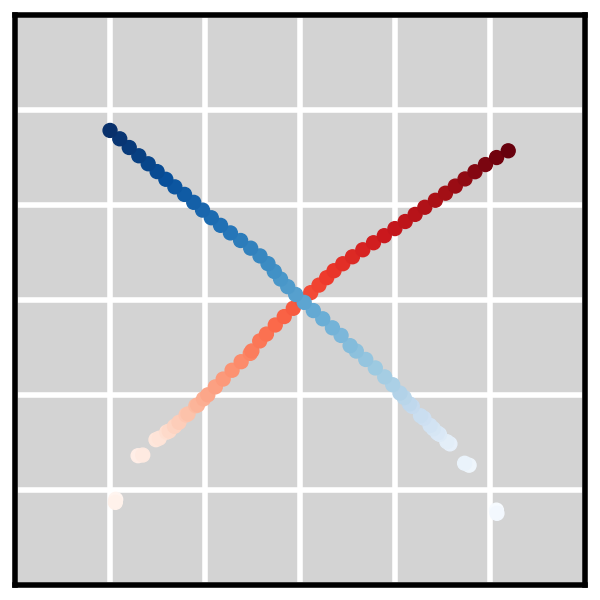
\includegraphics[width=\linewidth]{figures/w_memory.png}
        \caption{W/ memory} \label{fig:compositionality_w_memory}
    \end{subfigure}
    \begin{subfigure}[t]{.3\linewidth}
        \centering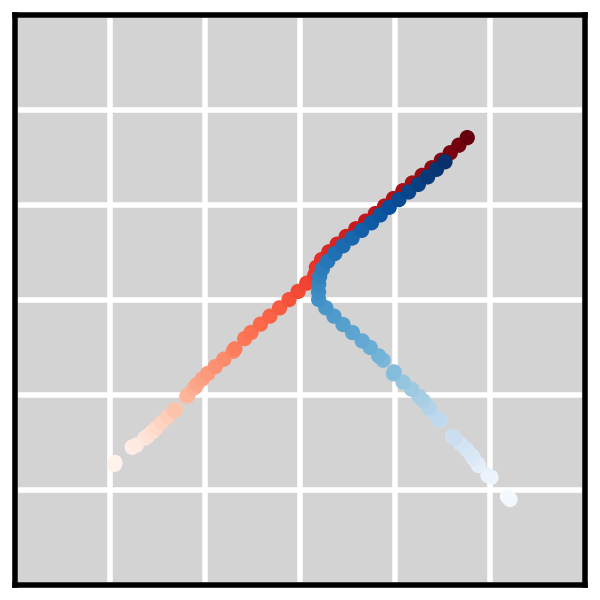
\includegraphics[width=\linewidth]{figures/wo_memory_v2.png}
        \caption{W/o memory} \label{fig:compositionality_wo_memory}
    \end{subfigure}
    \caption{Given a dataset of trajectories~(\subref{fig:compositionality_dataset}), \algo{} models the joint distribution of all subsequences of arbitrary length. At sampling time, we can sample from the trajectory distribution by sampling \algo{} with full horizon~(\subref{fig:compositionality_w_memory}) or recover Markovian dynamics by disregarding previous states~(\subref{fig:compositionality_wo_memory}).}
    \label{fig:compositionality}
\end{figure}



\subsection{Additional results in video prediction (wo/ cherry picking)}
\paragraph{Infinite Rollout without sliding window}
\algo{} can rollout longer than maximum training horizon\emph{without sliding window}. That is, we run \algo{}'s RNN continuously without ever reinitializing $\bz_0$. This is a surprising effect we observed from the rollout stabilization property of \algo{}. In Figure~\ref{fig:minecraft_long_0},~\ref{fig:dmlab_long_0}, we use \algo{} to generate video sequences of length $180$ and visualize subsampled sequences. Notably, \algo{} used in these visualizations is trained with a maximum length of $72$ frames for Minecraft and $36$ frames for DMLab, illustrating it can rollout 2x-5x times longer than it's trained on \emph{without sliding window}. In addition, we also tried rolling these models out for $2000$ frames and without seeing the model blowing up on both datasets. There are occasional cases where the Minecraft agent gets stuck and the entire screen is the ``dirt'' block, but this is more of a dataset issue~\ref{app:dataset_detail} and the agent is able to recover after it turns around. 

\begin{figure}[h]
    \centering
    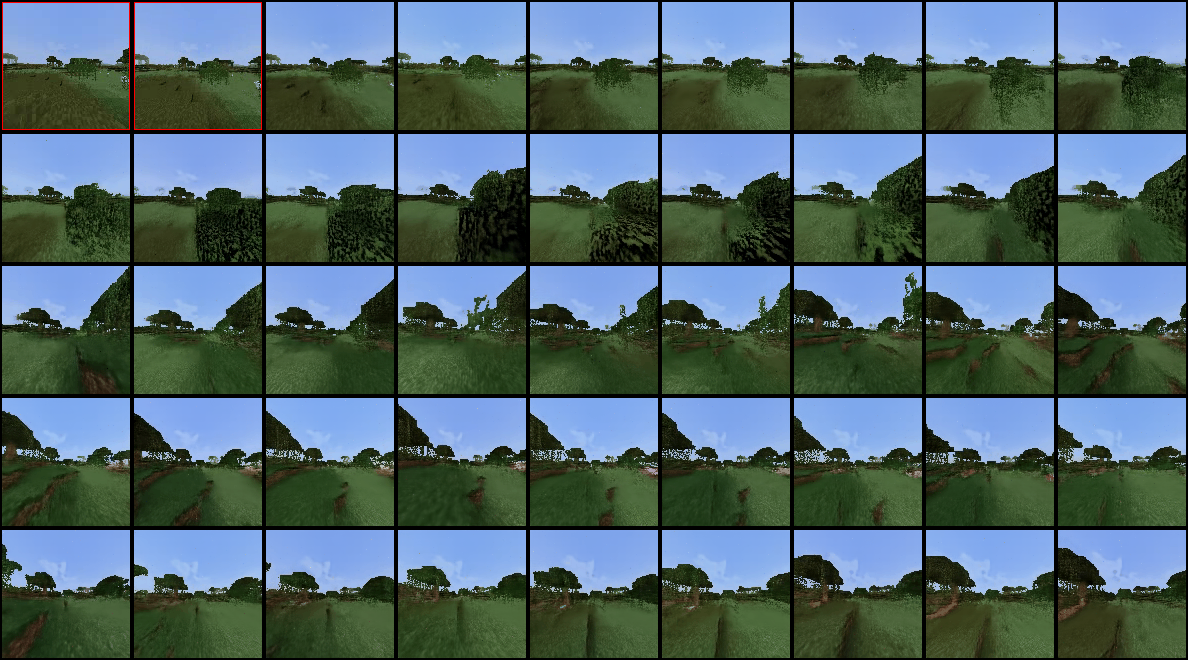
\includegraphics[width=\textwidth]{figures/appendix_vis/df_minecraft_long_1.png}
    \caption{Visualization shows \algo{} trained on $72$ frames is able to rollout $180$ frames on Minecraft dataset \emph{without sliding window}. The visualization shows a non-cherry-picked subsampling of these $180$ frames, although \algo{} can roll out much longer (such as 2000 frames) on this dataset.}
    \label{fig:minecraft_long_0}
\end{figure}
\begin{figure}[h]
    \centering
    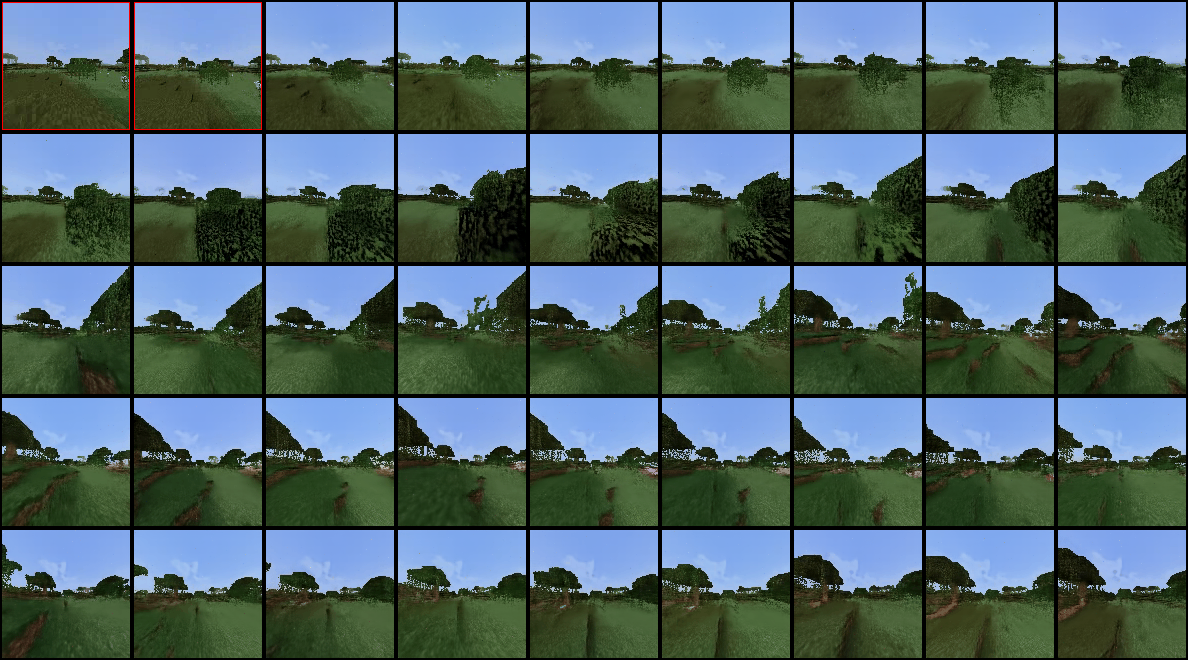
\includegraphics[width=\textwidth]{figures/appendix_vis/df_minecraft_long_1.png}
    \caption{\algo{} trained on $72$ frames is able to rollout $180$ frames on Minecraft dataset \emph{without sliding window}. The visualization shows a non-cherry-picked subsampling of these $180$ frames, although \algo{} can roll out much longer (such as 2000 frames) on this dataset. The first few frames marked in red are the ground truth images of the dataset used for conditioning.}
    \label{fig:minecraft_long_1}
\end{figure}
\begin{figure}[h]
    \centering
    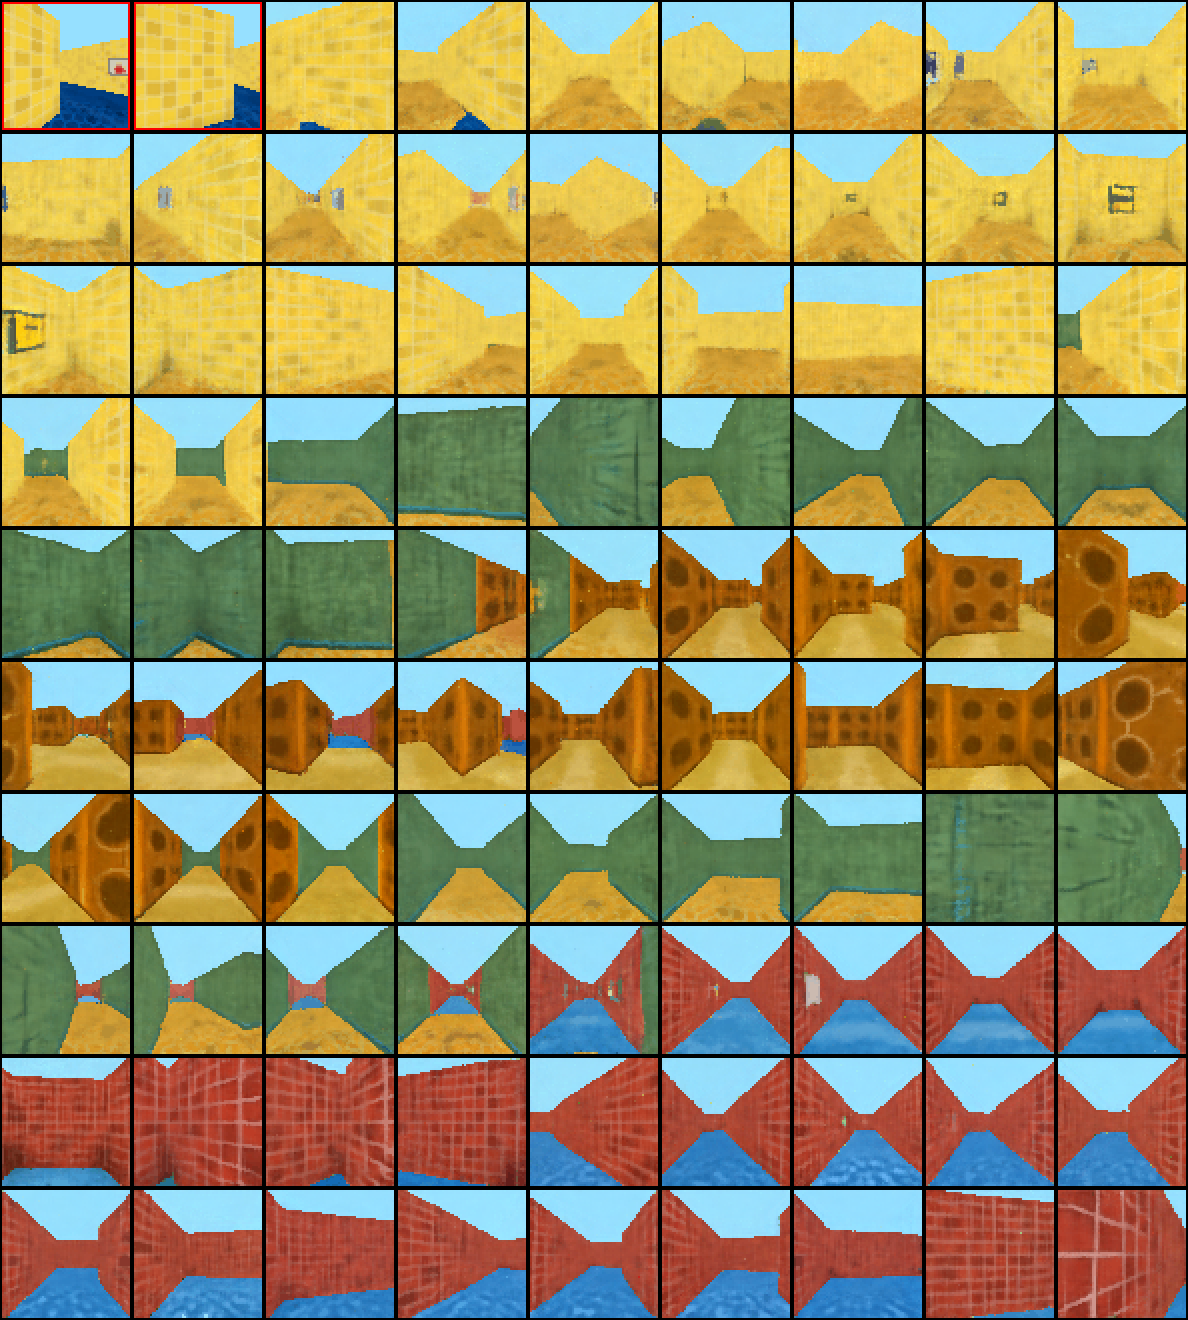
\includegraphics[width=\textwidth]{figures/appendix_vis/df_dmlab_long_0.png}
    \caption{Visualization shows \algo{} trained on $36$ frames is able to rollout $180$ frames on DMLab dataset \emph{without sliding window}. The visualization shows a non-cherry-picked subsampling of these $180$ frames, although \algo{} can roll out almost infinitely on this dataset. The first few frames marked in red are the ground truth images of the dataset used for conditioning.}
    \label{fig:dmlab_long_0}
\end{figure}
\begin{figure}[h]
    \centering
    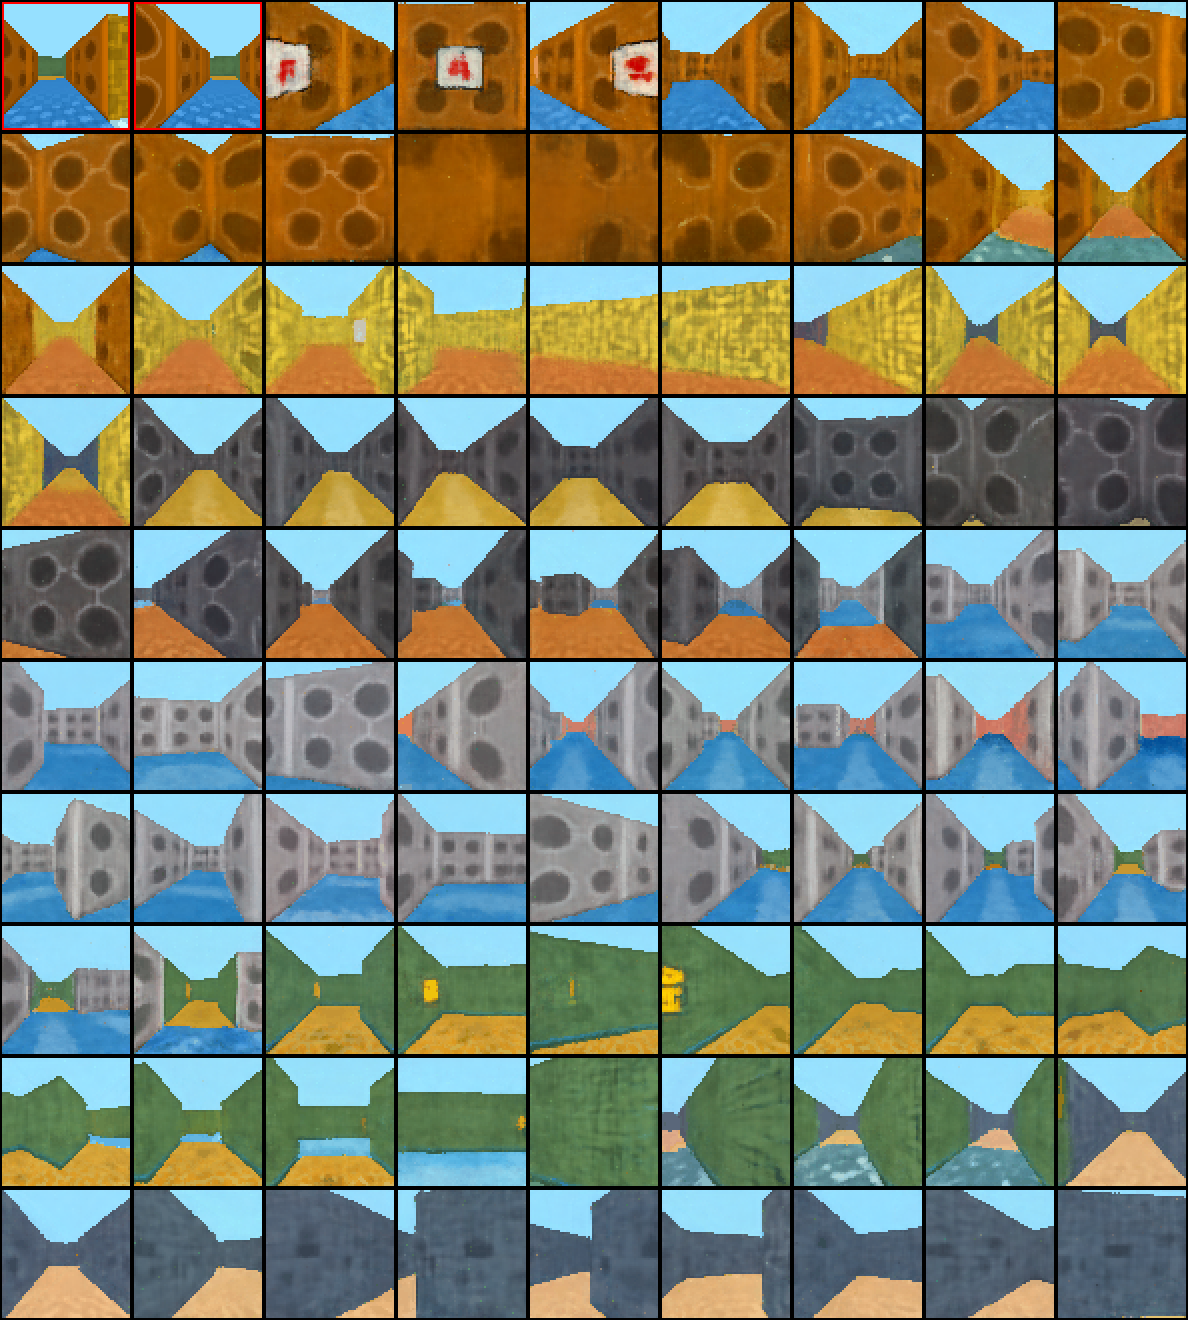
\includegraphics[width=\textwidth]{figures/appendix_vis/df_dmlab_long_1.png}
    \caption{Visualization shows \algo{} trained on $36$ frames is able to rollout $180$ frames on DMLab dataset \emph{without sliding window}. The visualization shows a non-cherry-picked subsampling of these $180$ frames, although \algo{} can roll out almost infinitely on this dataset. The first few frames marked in red are the ground truth images of the dataset used for conditioning.}
    \label{fig:dmlab_long_1}
\end{figure}

\paragraph{Consistency}
We also present additional results where we only generate within our maximum training length. As shown in figure~\ref{fig:minecraft_short}~\ref{fig:dmlab_short}, \algo{} can generate consistent videos. Results are not cherry-picked.
\begin{figure}[h]
    \centering
    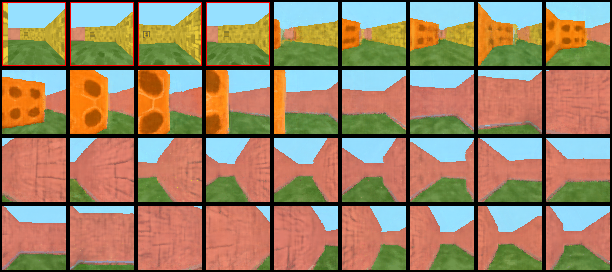
\includegraphics[width=\textwidth]{figures/appendix_vis/dmlab_df_0.png}
    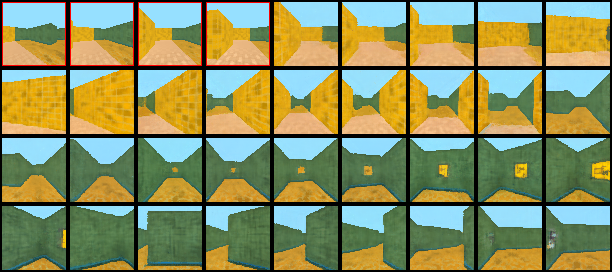
\includegraphics[width=\textwidth]{figures/appendix_vis/dmlab_df_1.png}
    \caption{Additional non-cherry-picked video prediction results on DMLab dataset, generated within maximum training length. The first few frames marked in red are the ground truth images of the dataset used for conditioning.}
    \label{fig:dmlab_short}
\end{figure}

\begin{figure}[h]
    \centering
    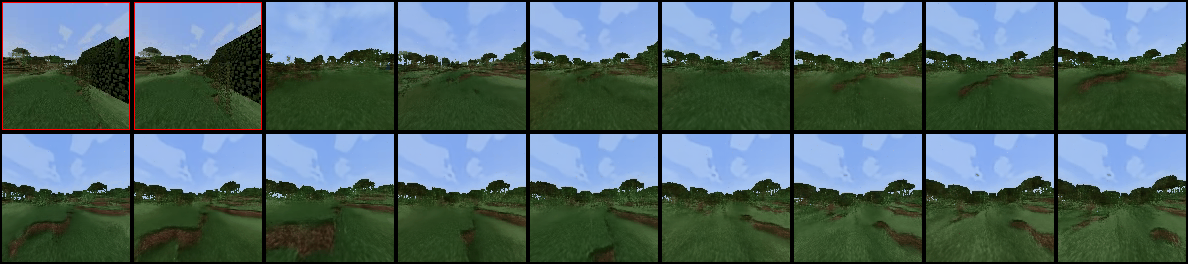
\includegraphics[width=\textwidth]{figures/appendix_vis/minecraft_df_0.png}
    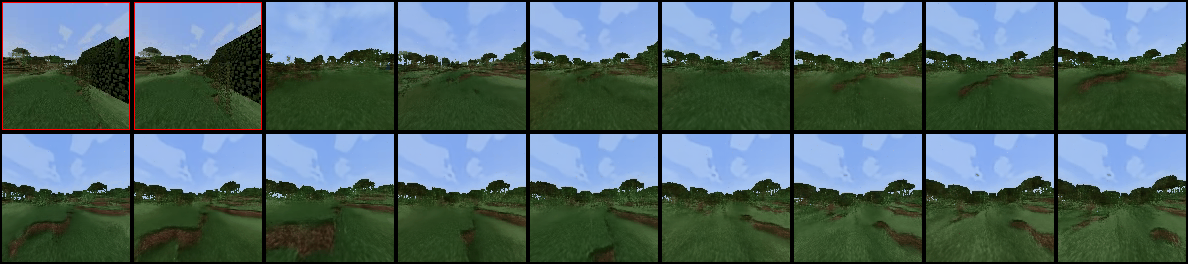
\includegraphics[width=\textwidth]{figures/appendix_vis/minecraft_df_0.png}
    \caption{Additional non-cherry-picked video prediction results on the Minecraft dataset, generated within maximum training length. The first few frames marked in red are the ground truth images of the dataset used for conditioning.}
    \label{fig:minecraft_short}
\end{figure}


\newpage

\subsection{Additional results in planning}
We provide some additional visualizations of causal planning in ~\ref{fig:df_plans_additional}. We also present additional visualization of \algo{} performing model predictive control in action. As shown in figure~\ref{fig:mpc_medium_0}, \algo{} can generate plans of shorter horizons since it's flexible horizon.
\begin{figure}[t]
    \centering
    \includegraphics[width=\textwidth]{figures/appendix_vis/df_medium_close_mpc.png}
    \caption{Example MPC planning for maze medium environment. Blue indicated trajectories actually executed already. Red is the plan.}
    \label{fig:mpc_medium_0}
\end{figure}

\begin{figure}[t]
    \centering
    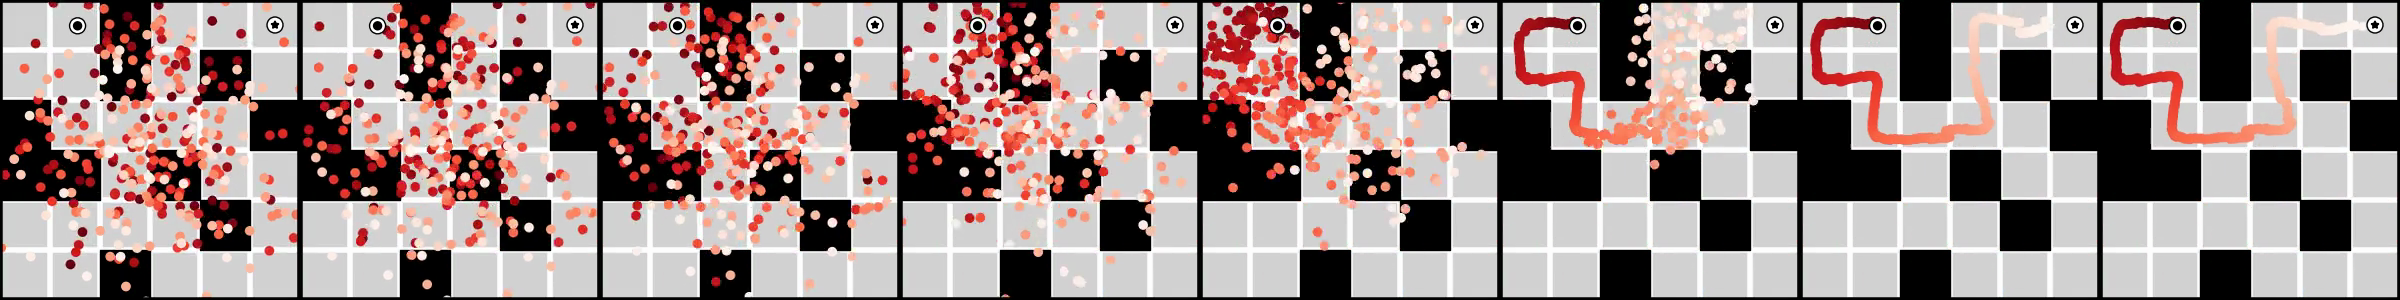
\includegraphics[width=\textwidth]{figures/appendix_vis/df_medium_close.png}
    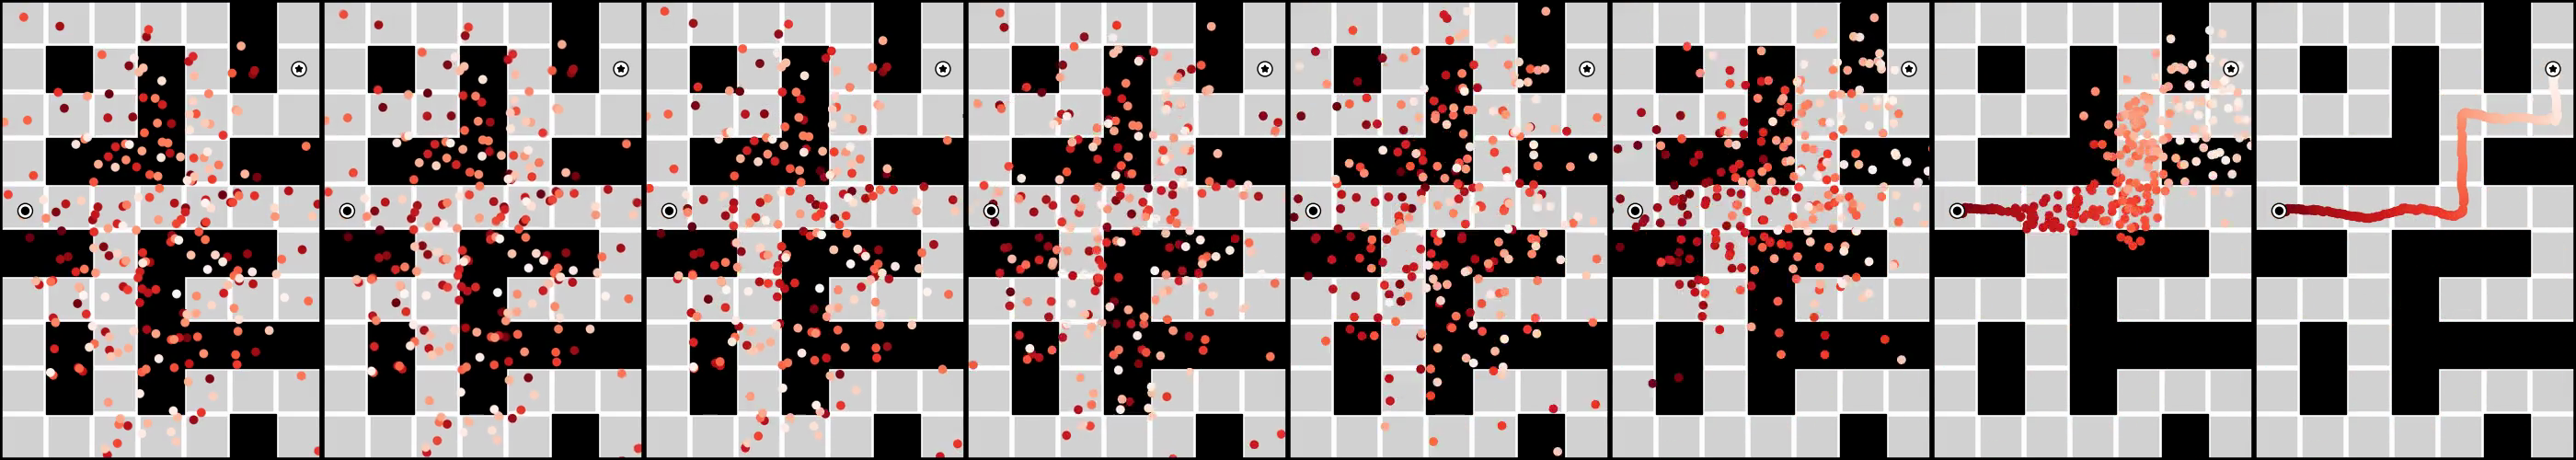
\includegraphics[width=\textwidth]{figures/appendix_vis/df_large_close.png}
    \caption{Example plans generated for maze medium (above) and maze large (below) environments.}
    \label{fig:df_plans_additional}
\end{figure}
\newpage

\subsection{Real robot experiment setup}
In Figure~\ref{fig:robot_currupted} we visualize our robot experiment setup with corruption on observation. The dataset is collected when the target bag isn't present, while we test with such a bag in the scene zero-shot for the imitation learning experiment with observation corruption. The typical failure mode is when the robot no longer reacts to the visual clues of the randomized location of objects. We didn't observe the robot act wildly due to visual distractors.

\begin{figure}[h]
    \centering
    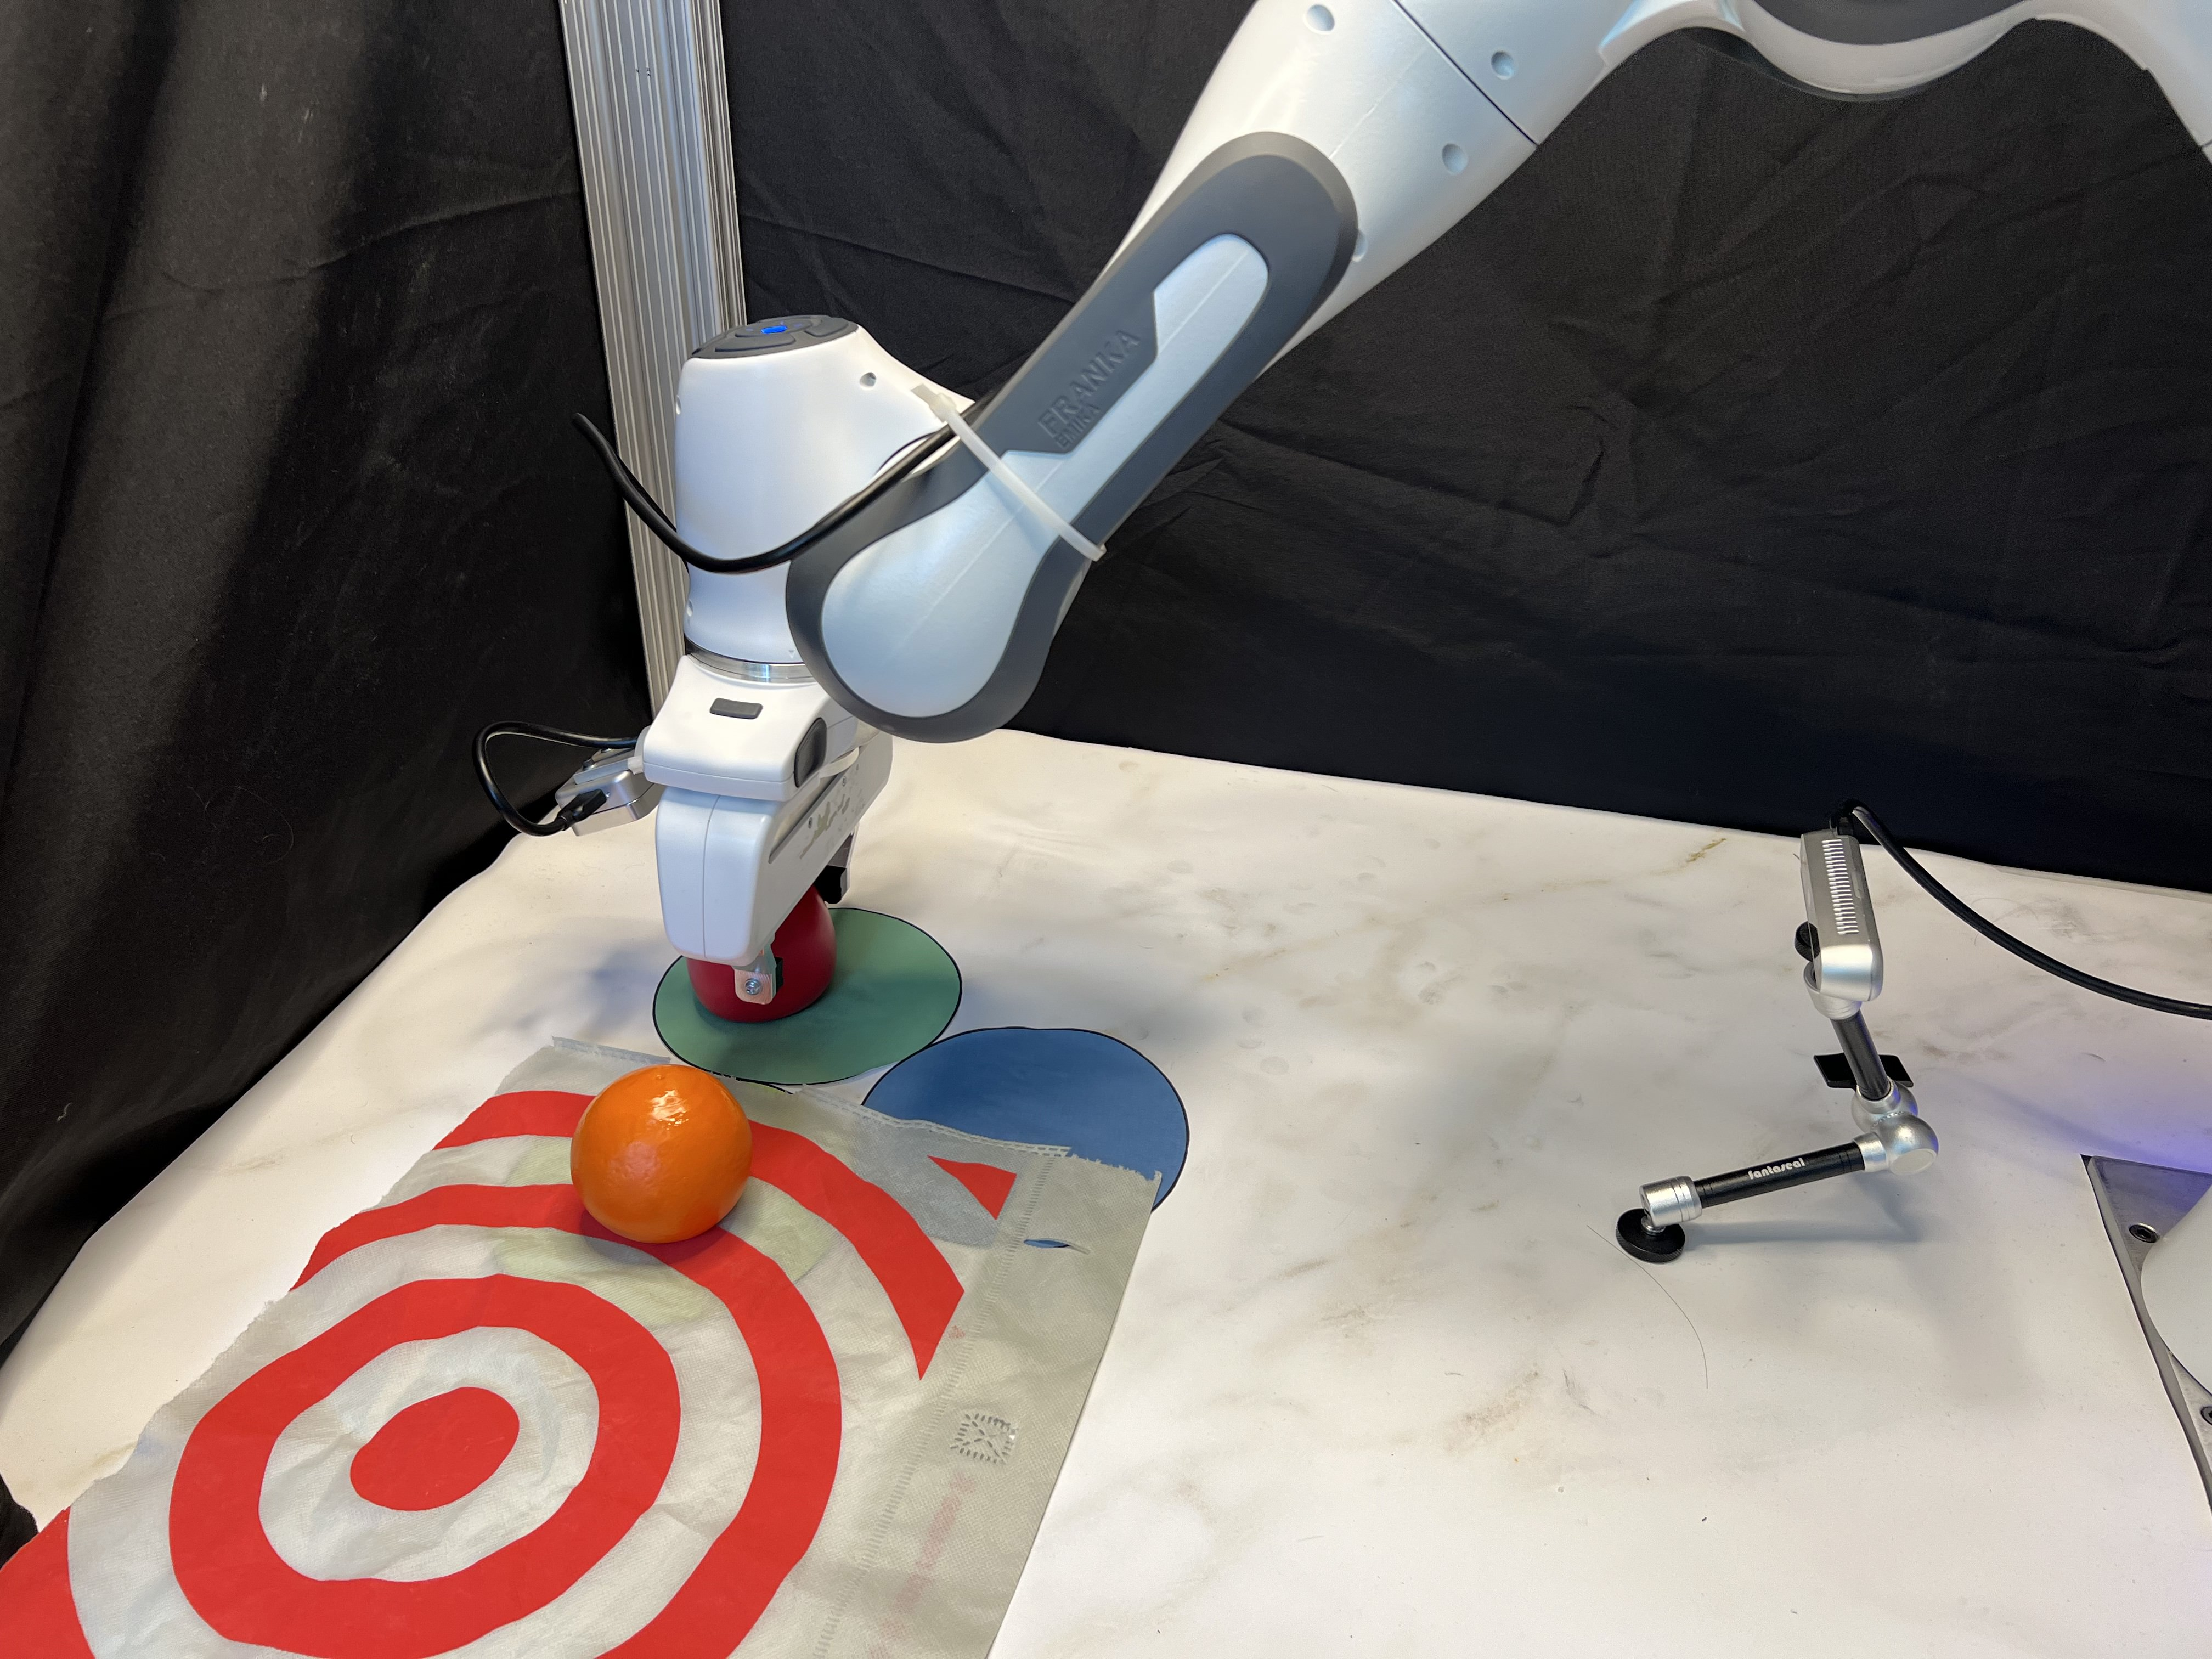
\includegraphics[width=0.5\textwidth]{figures/appendix_vis/robot_corrupt.jpg}
    \caption{We randomly throw a target bag on the table as a strong visual distractor. \algo{} can be prompted to treat observation as corrupted rather than ground truth.}
    \label{fig:robot_currupted}
\end{figure}

\label{app:dataset_detail}
\section{Additional details about datasets}
\subsection{Dataset for video diffusion}
We adopt the video prediction dataset Minecraft and DMlab used by TECO\cite{yan2023temporally}.

\paragraph{Minecraft Navigation}
The Minecraft navigation dataset consists of first-person-view videos of random walks in the Minecraft `swamp` biome. The agent walks via a technique called `sprint jump` which allows it to jump across blocks without getting stuck at 1 block obstacles. The agent walks straight most of the time, with small chances of turning left or right. The height and width of the video is $128$ pixels and we trim long videos to subsequences of $72$ frames. The dataset comes with paired action data but we discard them to bring more stochasticity to the prediction task. Due to limited compute, we only train on about $10\%$ of the total subsequences.

One problem we noticed about the dataset is when the agent runs into obstacles with a height of 2 blocks or more. In this case, the agent will get stuck and the entire video sequence will consist of grey granite patterns or brown dirty patterns. This leads to a huge amount of frames with these patterns, making video models predict meaningless frames. Yet, we deem this as a problem of this dataset itself.  

\paragraph{DMLab Navigation}
Deepmind Lab navigation dataset consists of random walks in a 3D maze environment. For DMLab, the resolution is $64$ pixels and we use subsequences of $48$ frames. We also disregard the provided actions due to training.

We note that the VQ-VAE latent that stable video diffusion~\cite{blattmann2023stable} diffuses is also only $128\times128\times 3$, indicating \algo{} has the potential to scale up to higher resolution images with pre-trained image encoder and decoders. Due to the sheer size of the datasets, we only use about $10\%$ of the total data sequences for training due to limited computing, as we observe that doing so already allows us to make good generations from initial frames from the test set.

\subsection{Dataset for planning}
\label{app:dataset_planning}
D4RL~\cite{d4rl} is a standard offline RL benchmark featuring a wide range of reinforcement learning environments. Each environment is associated with a provided dataset of offline interactions with the environment featuring state, action, and reward trajectories. 

Like Diffuer~\cite{janner2022planning}, we choose the 3 maze environments as they are challenging long-horizon, multi-modal, sparse reward problems uniquely suited for visualization and evaluating planning algorithms. The IDs for the 3 used environments are ``maze2d-medium-v1'', ``maze2d-large-v1'', ``maze2d-umaze-v1''. In each environment, one controls the acceleration of a robot to walk it towards a goal. The observation space is $4$ dimensional, featuring 2D location and velocity. The action space is 2D acceleration. The agent always receives a random start location and the goal is to reach a fixed goal position for each maze. The agent receives a reward of 1 if it is within a circle of radius 0.5 centered at the goal state, and 0 otherwise. 

The offline RL dataset for the maze environments consists of random walks in the maze. Specifically, the authors first designate all intersections and turn in the maze as waypoints and code an agent to navigate between waypoints with some randomization. As a result, the random walks are generated in a way that the path is collision-free with the walls. The random walks introduce stochasticity to the dataset, as trajectories in the dataset are never towards a specific goal. 

There are a few choices adopted from our main baseline Diffuser~\cite{janner2022planning}: we disregard the reward in the dataset and plan with goals only. We also evaluate a multi-goal variant of each environment (labeled as ``multi'' in Table~\ref{fig:planning}), where the goal is randomized just like the starting position. 

\subsection{Dataset for robot learning}
We choose a long horizon robotic manipulation task as described in Section~\ref{sec:exp_robot}: Consider a tabletop with three slots where we can place objects. One places an apple at slot A or slot B randomly, and then places an orange at the other slot between A and B. A robot is challenged to swap the position of two fruits using the third slot C. That is, it can only move a fruit to an empty slot at a time. For example, when the apple is at slot A and the orange is at slot B, it may move the apple to slot C, leaving slot A empty. Then move the orange to slot A and finally move the apple from slot C to slot B. In figure~\ref{fig:robot}, we illustrate the non-markovian property of the task: When the apple is at slot B and the orange is at slot C, one cannot tell what the immediate action is without knowing the initial positions of objects.

We put stickers on the table indicating a circular region occupied by any slot. Each circular region is designed to be about double the diameter of a fruit. To make sure the task requires visual feedback, we also randomize the location of a fruit inside the slot. We collected $150$ expert demonstrations of a Franka robot performing the task using VR teleoperation and impedance control. Among them, each initial slot configuration makes up half of the dataset. We record videos from two camera views, one from a hand camera and one in the front capturing all three slots. Each demonstration also comes with $6$ dof actions of the robot hand. During the data collection, since one successful demonstration will swap the position of two objects, its end configuration will naturally serve as the starting configuration of the other randomized location, which we leverage to save time. 

Each demonstration comprises $500-600$ frames and actions. We train \algo{} on the entire sequence. However, since adjacent frames are visually close, we pad and downsample the videos to $40$ frames where each frame is bundled with $15$ actions. 


\subsection{Dataset for time series }
\label{app:dataset_timeseries}
\ctable[
    caption = {Characteristics of the GluonTS datasets used to benchmark \algo{} in the domain of time series forecasting.},
    label = {tab:ts_data},
    pos = ht,
    doinside = \scriptsize,
    center,
    star
]{lccccc}{}{
    \FL
    Dataset & Dimension & Domain & Frequency & Steps & Prediction length
    \ML
    Exchange         & 8             & $\mathbb{R}^+$  & BUSINESS DAY            & 6,071 & 30 \NN
    Solar            & 137           & $\mathbb{R}^+$  & HOUR           & 7,009 & 24 \NN
    Electricity      & 370           & $\mathbb{R}^+$  & HOUR           & 5,833 & 24 \NN
    Traffic          & 963           & (0,1)           & HOUR           & 4,001 & 24 \NN
    Taxi             & 1,214         & $\mathbb{N}$     & 30-MIN         & 1,488 & 24 \NN
    Wikipedia        & 2,000         & $\mathbb{N}$     & DAY            & 792 & 30
    \LL
}

We use a set of time series datasets accessible via GluonTS~\cite{gluonts}, which are adopted from prior works like \cite{DBLP:journals/corr/YuRD15,DBLP:journals/corr/LaiCYL17,SALINAS20201181}. These datasets capture real-world data of high-dimensional dynamics like monetary exchange rates or the electricity grid. In Table~\ref{tab:ts_data}, we provide a summary of the features of these datasets, such as the dimensionality, the domains, the sampling frequency, the length of the multivariate sequence in the training set, and the prediction length. We access the datasets in Table~\ref{tab:ts_data} via GluonTS and wrap the data processing functions implemented in GluonTS in our own dataloaders. Each dataset consists of one long multivariate sequence, which is the training split, and a set of short sequences that make up the test split. We construct a validation set of the same cardinality as the held-out test set as a randomly sampled subset of subsequences from the training set. All splits are normalized by the mean and the standard deviation of the features in the training split.

\paragraph{Covariates}
Often, statistical models that approximate~\eqref{eq:prediction_pdf} benefit from manually curated features as additional input to the observations. A sequence of covariates $\boldsymbol{C} = \left\{ \mathbf{c}_t \right\}_{t=1}^T$ can be constructed to help the model recognize seasonal patterns and other temporal dependencies. We follow the implementation in~\cite{rasul2021multivariate} to construct the covariate sequence as a function of the frequency of each dataset in Table~\ref{tab:ts_data}. As such, our covariates are composed of lagged inputs, as well as learned embeddings and handcrafted temporal features that encode information such as the hour of the day or the day of the month, depending on the sampling rate of the particular time series that is being modeled. Therefore, covariates are known for the entire interval~$\left[1, T\right]$, even at inference. We can easily incorporate covariates into the probabilistic framework as
\begin{equation} \label{eq:prediction_pdf_covariates}
    q{\left( \mathbf{x}_{t_0:T} \mid \mathbf{x}_{1:t_0-1}, \mathbf{c}_{1:T} \right)} := \prod_{t=t_0}^T{q{\left( \mathbf{x}_t \mid \mathbf{x}_{1:t_0-1}, \mathbf{c}_{1:T} \right)}} \text{.}
\end{equation}
The benefit obtained from covariates is highly dependent on the characteristics of both the dataset and the model used, as well as the feature engineering practices followed.


\paragraph{Metric}
The Continuous Ranked Probability Score (CRPS)~\cite{james1976scoring} is a scoring function that measures how well the forecast distribution matches the ground truth distribution:
\begin{equation*}
    \operatorname{CRPS}(F, x) = \int_\mathbb{R} \left(F(z) - \mathbb{I}\left\{ x \leq z \right\} \right)^2 \dd{z} \text{,}
\end{equation*}
where $F(z)$ is the univariate cumulative distribution function (CDF) over the predicted value, $x$ is a ground truth observation, and $\mathbb{I}\left\{ x \leq z \right\}$ is the indicator function that is one if $x \leq z$ and zero otherwise. By summing the $D$-dimensional time series along the feature dimension for simulated samples (resulting in $\hat{F}_\text{sum}(t)$) and ground truth data (as $\sum_i x^0_{i,t}$), we can report the $\operatorname{CRPS}_\text{sum}$
\begin{equation*}
    \operatorname{CRPS}_\text{sum} = \mathbb{E}_{t \sim \mathcal{U}\left(t_0, T\right)} \left[\operatorname{CRPS}{\left(\hat{F}_\text{sum}(t), \sum_i x^0_{i,t} \right)}\right]
\end{equation*}
as the average over the prediction window. The lower the $\operatorname{CRPS}_\text{sum}$ value, the better the predicted distribution match the data distribution.

First, we manually sum the time series along the feature dimension and estimate the CDF $\hat{F}_\text{sum}(t)$ via 19 quantile levels at each time step $t$ from 100 sampled trajectories. We then use the implementation in GluonTs~\cite{gluonts} to compute the $\operatorname{CRPS}$, which we report as $\operatorname{CRPS}_\text{sum}$ in Table~\ref{tab:results_ts}. While we aggregate the data manually, we verify that the numerical error relative to the GluonTS implementation remains orders of magnitude below the precision threshold of the reported metric.





\end{document}
